\documentclass[20pt,landscape,footrule,headrule]{foils}
\usepackage[usenames]{color}
\usepackage[export]{adjustbox}
\usepackage{latexsym}
\usepackage{amsmath}
\usepackage{graphicx,color}  %needed to \includegraphics
\usepackage{amssymb}
\usepackage{multirow}
\usepackage{multicol}
\usepackage{polynom}
\usepackage{tabularx}
\usepackage{threeparttable}
\usepackage{siunitx}
\usepackage{ulem}
\usepackage{colortbl}
\usepackage{multirow}
\usepackage{hhline}
\usepackage{calc}
\usepackage{array}
%\usepackage{caption}
\newcommand{\newl}{\newline\newline}
\newcommand{\GN}{\mathbb{N}}
\newcommand{\GZ}{\mathbb{Z}}
\newcommand{\GQ}{\mathbb{Q}}
\newcommand{\GR}{\mathbb{R}}
\pagenumbering{arabic}

\newcommand{\crois}{\nearrow}
\newcommand{\decrois}{\searrow}

\newcommand{\cch}{\setlength{\unitlength}{0.2mm}
\begin{picture}(25,25)
\thicklines
\curve(0,0,15,7,25,23)
\end{picture}}

\newcommand{\ccb}{\setlength{\unitlength}{0.2mm}
\begin{picture}(25,25)
\thicklines
\curve(0,0,7,15,25,23)
\end{picture}}

\newcommand{\dch}{\setlength{\unitlength}{0.2mm}
\begin{picture}(25,25)
\thicklines
\curve(0,23,10,7,25,0)
\end{picture}}

\newcommand{\dcb}{\setlength{\unitlength}{0.2mm}
\begin{picture}(25,25)
\thicklines
\curve(0,23,15,18,25,0)
\end{picture}}

\usepackage{epic}
\usepackage{curves}


\usepackage[utf8]{inputenc}
\usepackage{xcolor}
\usepackage{newunicodechar}

\newcommand\Warning{%
 \makebox[1.4em][c]{%
 \makebox[0pt][c]{\raisebox{.1em}{!}}%
 \makebox[0pt][c]{\color{red}\Large$\bigtriangleup$}}}%


\newcommand{\localtextbulletone}{{\raisebox{.45ex}{\rule{.6ex}{.6ex}}}}
\renewcommand{\labelitemi}{\localtextbulletone}

\DeclareMathOperator{\pgdc}{pgdc}
\DeclareMathOperator{\card}{card}
\DeclareMathOperator{\sgn}{sgn}
\DeclareMathOperator{\SG}{SG}
\DeclareMathOperator{\lo}{lo}
\DeclareMathOperator{\IC}{I.C.}
\DeclareMathOperator{\ID}{I.D.}
\DeclareMathOperator{\IH}{I.H.}
\DeclareMathOperator{\IB}{I.B.}
\DeclareMathOperator{\INF}{INFL}
\DeclareMathOperator{\SC}{S.C.}
\DeclareMathOperator{\SP}{S.P.}
\DeclareMathOperator{\cosec}{cosec}
\DeclareMathOperator{\cotg}{cotg}
\DeclareMathOperator{\tg}{tg}
\DeclareMathOperator{\tgh}{tgh}
\DeclareMathOperator{\sech}{sech}
\DeclareMathOperator{\cosech}{cosech}
\DeclareMathOperator{\cotgh}{cotgh}

%%%%%%%%%%%%%%%%%%%%%%%%%%%%%%%%%%%%%%%%%%%%%

%%%%%%%%%%%%%%%%%%%%%%%%%%%%%%%%%%%%%%%%%%%%%%%%%%%%%%%

\input def

%\usepackage[T1]{fontenc}

\def\filedate{Fall 2020}
\def\fh{\foilhead}
\def\me{P.Boily (uOttawa, IACS, DAL) \\ with Y.Cissokkho, S.Fadel, R.Millson, R.Pourhasan}
\def\code{MAT 4376/5314E \\ Techniques of Data Analysis}
\def\codee{MAT 4376/5314E}
\def\descr{Techniques of Data Analysis}
\def\lec{}
\def\sec{6}
\def\sections{}
\def\sectitle{Anomaly Detection and Outlier Analysis}
\def\unitofstudy{\codee\ -- \descr}
\def\mc{\mathcal}
\def\rfh{\rotatefoilhead}
\title{\code \\ \ \\  Module \sec\\ \sectitle}
\author{\me}
\date{\filedate}
\definecolor{burgundy}{rgb}{0.6, 0.0, 0}
\definecolor{bleudefrance}{rgb}{0, 0, 0.6}
\definecolor{darkestgreen}{rgb}{0.25, 0.5, 0.25}
\definecolor{grey}{rgb}{0.5, 0.5, 0.5}
%\setlength{\parskip}{50pt}

\begin{document}
\maketitle \MyLogo{Anomaly Detection and Outlier Analysis}
\leftheader{\unitofstudy} \rightheader{Module \sec\ -- \sectitle}
\rightfooter{\quad\textsf{\thepage}} % this is the default

  \providecommand{\huxb}[2]{\arrayrulecolor[RGB]{#1}\global\arrayrulewidth=#2pt}
  \providecommand{\huxvb}[2]{\color[RGB]{#1}\vrule width #2pt}
  \providecommand{\huxtpad}[1]{\rule{0pt}{#1}}
  \providecommand{\huxbpad}[1]{\rule[-#1]{0pt}{#1}}

\fh{\textcolor{darkestgreen}{Outline}}
\noindent With the advent of automatic data collection, it is now possible to store and process large troves of data. There are technical issues associated to massive data sets, such as the speed and efficiency of analytical methods, but there are also problems related to the detection of \textbf{anomalous observations} and the \textbf{analysis of outliers}.  \newl Unexpected observations can spoil analysises and/or be indicative of data collection and data processing issues.\ \\ \ \\  Extreme and irregular values behave very differently from the majority of observations: they can represent criminal attacks, fraud attempts, targeted attacks, or data collection errors. As a result, anomaly detection and outlier analysis play a crucial role in cyber-security, quality control, etc.   
\newpage\ \\ \noindent 
6.1 -- Basic Notions and Overview (p.\pageref{6.1}) \\ \small  
\textcolor{white}{ab} \localtextbulletone\ Anomaly Detection as Statistical Learning  (p.\@\pageref{6.1.1}) 
\normalsize \ \\ \ \\  
 6.2 -- Quantitative Methods of Anomaly Detection  (p.\pageref{6.2}) \\ \small
\textcolor{white}{ab} \localtextbulletone\ Distance-Based Methods (p.\@\pageref{6.2.1}) \\ 
\textcolor{white}{ab} \localtextbulletone\ Density-Based Methods (p.\@\pageref{6.2.2}) 
\normalsize \ \\ \ \\  
6.3 -- Qualitative Methods (p.\pageref{6.3}) \\ \small
\textcolor{white}{ab} \localtextbulletone\ AVF Algorithm (p.\@\pageref{6.3.1}) \\ 
\textcolor{white}{ab} \localtextbulletone\ Greedy Algorithm (p.\@\pageref{6.3.2}) 
\normalsize \ \\ \ \\ 
6.4 -- Anomalies in High-Dimensional Datasets (p.\pageref{6.4}) \\ 
\small
\textcolor{white}{ab} \localtextbulletone\ Definitions and Challenges (p.\@\pageref{6.4.1}) \\ 
\textcolor{white}{ab} \localtextbulletone\ Projection-Based Methods (p.\@\pageref{6.4.2}) \\ 
\textcolor{white}{ab} \localtextbulletone\ Subspace  Methods (p.\@\pageref{6.4.3}) 
\normalsize
\newpage\ \\ \noindent 
6.5 -- Applications  (p.\pageref{6.5}) \\ 
\small
\textcolor{white}{ab} \localtextbulletone\ S\&P 500 (p.\@\pageref{6.5.1}) \\ 
\textcolor{white}{ab} \localtextbulletone\ Airports (p.\@\pageref{6.5.2}) \\ 
\textcolor{white}{ab} \localtextbulletone\ Application 3 (p.\@\pageref{6.5.3}) \\ 
\textcolor{white}{ab} \localtextbulletone\ Application 4 (p.\@\pageref{6.5.4}) \\ 
\textcolor{white}{ab} \localtextbulletone\ Application 5 (p.\@\pageref{6.5.5}) 
\normalsize \ \\ \ \\ 
6.6 -- Advanced Topics (p.\pageref{6.6}) \\ 
\small
\textcolor{white}{ab} \localtextbulletone\ Outlier Ensembles (p.\@\pageref{6.6.1}) \\ 
\textcolor{white}{ab} \localtextbulletone\ Anomalies in Text Datasets Methods (p.\@\pageref{6.6.2})\normalsize 
 \ \\ \ \\ 
References and other details can be found in Cissokho, Y., Fadel, S., Millson, R., Pourhasan, R., Boily, P. [2020], \textit{Anomaly Detection and Outlier Analysis}, Data Science Report Series, Data Action Lab.


\newpage
\begin{center}

\includegraphics[width=0.95\textwidth]{Images/fish.png}
\end{center}



\fh{\textcolor{darkestgreen}{6.1 -- Basic Notions and Overview}} \label{6.1}
\noindent Isaac Asimov, the prolific American author, once wrote that \begin{quote} The most exciting phrase to hear [...], the one that heralds the most discoveries, is not ``Eureka!'' but ``That's funny...''.\end{quote}

\noindent \textbf{Important Goals:} establish anomaly detection protocols  and to identify strategies to deal with such observations.

\noindent \textbf{Outlying observations:} data points that are atypical within-unit or between-units, or as part of a collective subset of observations. 

\noindent In other words, outliers are observations which are \textbf{dissimilar to other cases} or which contradict \textbf{known dependencies} or rules.

\newpage\ \\ \noindent Outlying observations may be anomalous along any of the individual variables, or in combination.
\begin{center}
    \rule{0.5\textwidth}{.4pt}
\end{center}
\noindent Observations could be anomalous in one context, but not in another: 
\begin{itemize}
\item an adult male who is 6-foot tall falls in the $86$th percentile among Canadian males $\Longrightarrow$ tall, but not unusually so; 
\item in Bolivia, the same man would land in the $99.9$th percentile $\Longrightarrow$ extremely tall; a rarity.
\end{itemize}
Anomaly detection points towards interesting questions for analysts and subject matter experts: in this case, why is there such a large discrepancy in the two populations?  
\newpage \ \\ \noindent
What's an \textbf{outlier/anomalous observation?} (reprise)
\begin{itemize}
\item \textbf{``bad'' object/measurement:} data artifacts, spelling mistakes, poorly imputed values, etc.
\item  \textbf{misclassified observation:} according to the existing data patterns: the observation should have been labeled differently in the 
\item  an observation whose measurements are found in the \textbf{distribution tails}, in a large enough number of features;
\item \textbf{unknown unknowns:} completely new type of observations whose existence was hertofore unsuspected.
\end{itemize}

\newpage\ \\ \noindent A common mistake that analysts make when dealing with outlying observations is to remove them from the dataset without carefully studying whether they are \textbf{influential data points}.\newl Influential observations are points whose absence leads to \textbf{markedly different} analysis results.
\newl Points can be influential for one analytical methods, but not for another. 
\newl \textbf{Remedial measures} (data transformation strategies, etc.) may need to be applied to minimize any undue effect. 
\newl Outliers may be influential, and influential data points may be outliers, but the conditions are \textbf{neither necessary nor sufficient}. 


\fh{Anomalies} 

\noindent Anomalies are \textbf{infrequent} and typically shrouded in \textbf{uncertainty} due to their relatively low numbers.  
\newl This makes it difficult to differentiate anomalies from banal \textbf{noise} or \textbf{data collection errors}. 
\newl The boundary between normal and deviant observations is usually \textbf{fuzzy}.
\newl \textbf{Example:} before the advent of e-shops, a purchase which was recorded at 3AM (local time) would probably raise a red flag for a credit card company; but with online shops, that is not necessarily the case. 
\newpage\ \\ \noindent If anomalies are actually associated with \textbf{malicious activities}, they are often \textbf{disguised} to blend in with normal observations $\Longrightarrow$ this obviously complicates the detection process.
\newl Numerous methods exist to identify anomalous observations; \textbf{none of them are foolproof} and judgement must be used. 
\newl \textbf{Graphical methods} to identify outliers are particularly easy to implement:
\begin{itemize}
\item boxplots, scatterplots, scatterplot matrices, and 2D tours
\end{itemize} usually require a  low-dimensional setting for  \textbf{interpretability}. 
\newl They also usually find those anomalies that ``\textbf{shout the loudest}'' [Baron]. 
\newpage
\begin{center}

\includegraphics[width=0.95\textwidth]{Images/fish.png}
\end{center}

\newpage\ 
\begin{center}
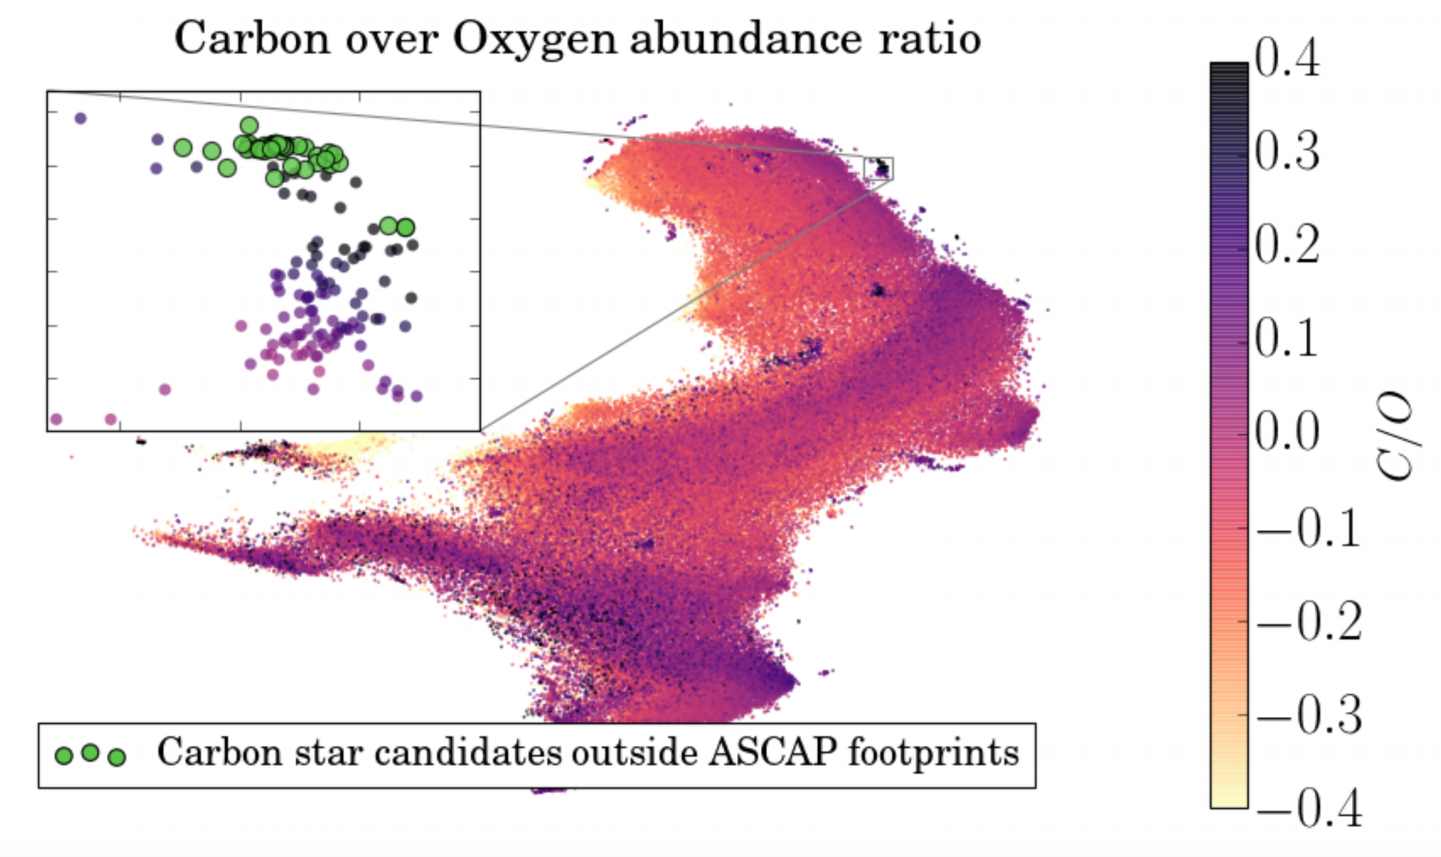
\includegraphics[width=0.8\textwidth]{Images/COar.png} \\ 
Derived-score anomaly detection may help (... or it may not) [Baron]
\end{center}

\newpage\ \\ \noindent
\textbf{Simple analytical methods} using Cooke's or Mahalanobis' distances are sometimes used, but more sophisticated analysis is usually required, especially when trying to identify influential points (\textit{cf.} \textbf{leverage}). 
\newl 
In small datasets, detection can be conducted on a case-by-case basis.\newl \textbf{Questions:} how many anomalies are too many to find? How many cases are you willing to inspect manually? 
\newl It is tempting to use \textbf{automated detection/removal} with large datasets, but doing so may be catastrophic from a data analysis perspective!
\newl If once ``anomalous'' observations have been removed from the dataset, previously ``regular'' observations can become anomalous in turn in the smaller dataset -- when does the runaway train?
\newpage\ \\ 
\begin{center}
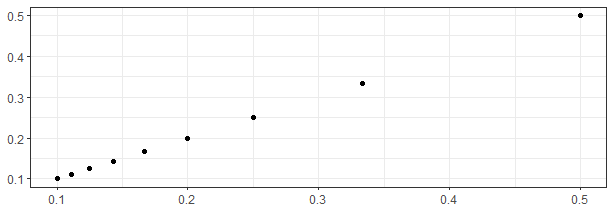
\includegraphics[width=\textwidth]{Images/ADOA1.png} \\ Automatic renewal of anomaly (step $1$)
\end{center}
\newpage\ \\ 
\begin{center}
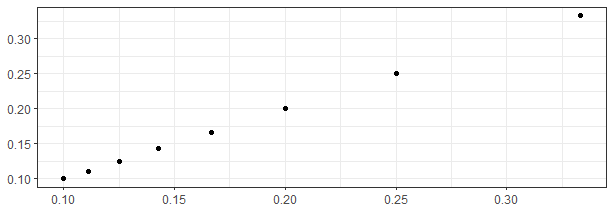
\includegraphics[width=\textwidth]{Images/ADOA2.png}\\ Automatic renewal of anomaly (step $2$)
\end{center}
\newpage\ \\ 
\begin{center}
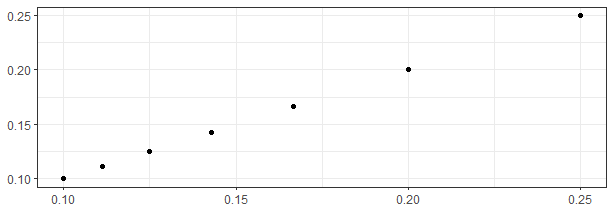
\includegraphics[width=\textwidth]{Images/ADOA3.png}\\ Automatic renewal of anomaly (step $3$)
\end{center}
\newpage\ \\ 
\begin{center}
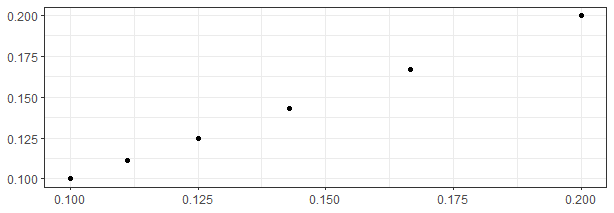
\includegraphics[width=\textwidth]{Images/ADOA4.png} \\ Automatic renewal of anomaly (step $4$)
\end{center}
\newpage\ \\ 
\begin{center}
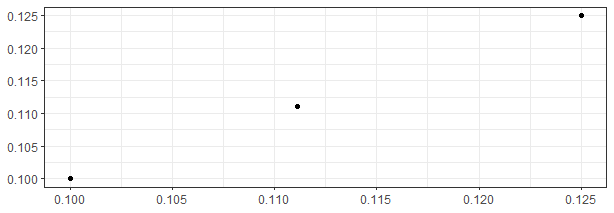
\includegraphics[width=\textwidth]{Images/ADOAn.png}\\ Automatic renewal of anomaly (step $n$)
\end{center}
\newpage\ \\ 
\begin{center}
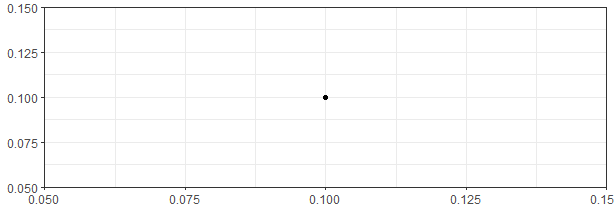
\includegraphics[width=\textwidth]{Images/ADOA10.png}\\ Automatic renewal of anomaly (step $9$)
\end{center}
\newpage\ \\ \noindent In the early stages of anomaly detection, we use \textbf{simple data analyses:}
\begin{itemize}
\item descriptive statistics, 
\item $1-$ and $2-$way tables, and  
\item traditional  visualizations.
\end{itemize}
The goal is to \textbf{help identify anomalous observations} and to \textbf{obtain insights about the data}.
\newl 
This leads to more sophisticated anomaly detection methods and could also could eventually lead to modifications of the analysis plan. 
\newl \textbf{THIS IS NEVER AN UNWELCOME DEVELOPMENT!}


\fh{Learning Framework} 
\noindent How are outliers detected, in practice? 
\newl Methods come in two flavours: 
\begin{itemize}
\item \textbf{supervised}, and 
\item \textbf{unsupervised}.\end{itemize}
\textbf{Supervised methods} (SL) use a historical record of \textbf{previously identified anomalous observations} to build a \textbf{predictive classification or regression model} which estimates the probability that a unit is anomalous.\newpage\ \begin{center}
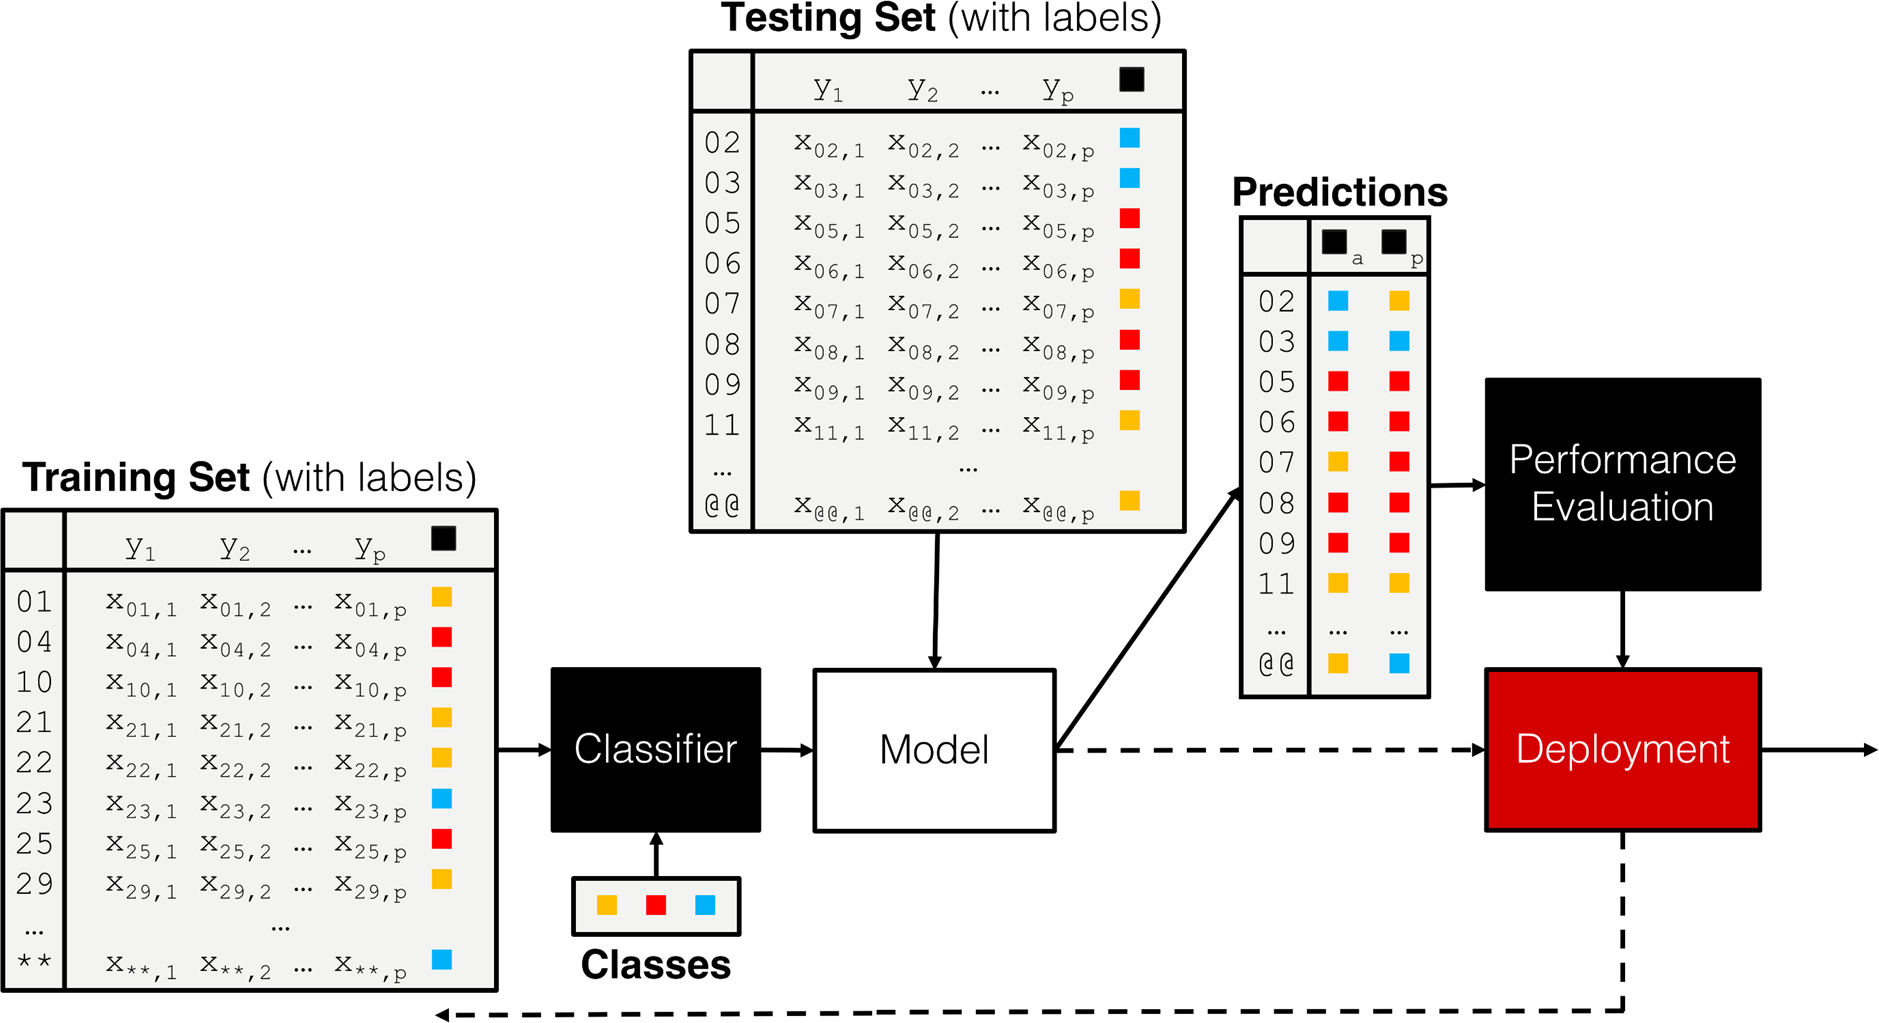
\includegraphics[width=\textwidth]{Images/Classification}
\end{center}
\newpage\ \\ \noindent  \textbf{SL Challenges:} 
\begin{itemize}
\item domain expertise and resources are required to tag the data;
\item since anomalies are typically \textbf{infrequent}, these models often also have to accommodate the \textbf{rare occurrence} (or class imbalance) problem, and 
\item SL methods need to minimize a \textbf{loss function} (cost of making a mistake) which is usually symmetrical (in the anomaly detection context, this  is not usually a valid assumption). 
\end{itemize}
Even more than in traditional analysis settings, anomaly detection can lead to \textbf{technically correct but ultimately useless} (non-actionable) \textbf{results}. 
\newpage
\begin{center}
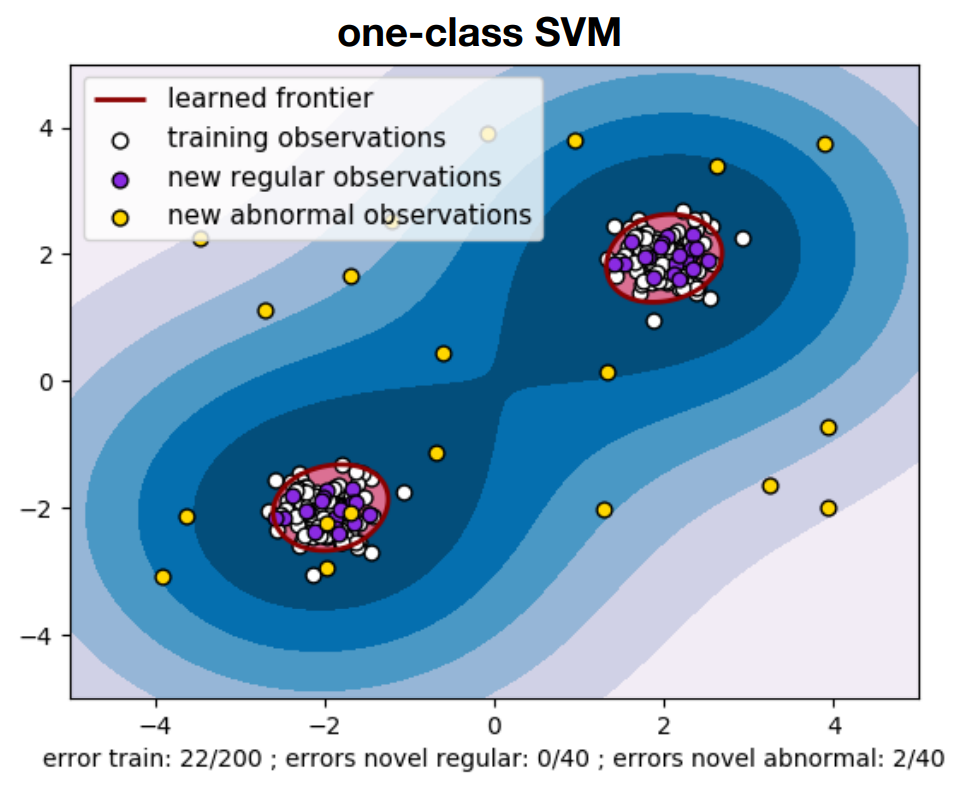
\includegraphics[width=0.68\textwidth]{Images/1SVM.png} \\ 
Learning an \textbf{anomaly frontier} [Baron].
\end{center}
\newpage\ \\ \noindent  \textbf{Example:} The vast majority ($99.999+$\%) of air passengers \textbf{do not} bring weapons with them on flights. \newl A model that predicts that no passenger is ever attempting to smuggle a weapon on board a flight would be $99.999+$\% accurate.\newl But it would miss the point \textbf{completely}. For the \textbf{security agency}, the cost of wrongly thinking that a passenger is:
\begin{itemize}
\item  smuggling a weapon $\Longrightarrow$ cost of a single search;
\item NOT smuggling a weapon $\Longrightarrow$ catastrophe (potentially). 
\end{itemize}
\noindent The wrongly targeted individuals may have a  ... somewhat different take on this, from a societal and personal perspective.

\newpage\ \\ \noindent \textbf{Unsupervised methods} (UL) \begin{itemize}
\item use no previously labeled (anomalous/non-anomalous) data, and 
\item try to determine if an observation anomalous solely by comparing its behaviour to that of the other observations. 
\end{itemize}
\textbf{Example:} if all workshop participants except for one can view the video conference lectures, then the one individual/internet connection/computer is \textbf{anomalous} -- it behaves in a manner which is different from  the others. \newl 
\textbf{VERY IMPORTANT NOTE:} this \textbf{DOES NOT} mean that the different behaviour is the one we are actually interested in/searching for! 
\newl Be weary: this is true of anomaly detection in data and in real-life. 
\newpage
\begin{center}

\includegraphics[width=0.95\textwidth]{Images/fish.png}
\end{center}

\fh{Traditional Outlier Detection Tests}
\noindent The most commonly-used test is \textbf{Tukey's} (univariate) \textbf{boxplot test}. Let $Q_1$ and $Q_3$ represent an observed feature's $1^{\textrm{st}}$ and $3^{\textrm{rd}}$ quartile, respectively.\newl For \textbf{normally distributed} measurements, regular observations typically lie between the \textbf{inner fences} $$Q_1-1.5(Q_3-Q_1) \quad\mbox{and}\quad Q_3+1.5(Q_3-Q_1).$$ \textbf{Suspected outliers} lie between the inner fences and their \textbf{outer fences} 
$$Q_1-3(Q_3-Q_1) \quad\mbox{and}\quad Q_3+3(Q_3-Q_1).$$
Points beyond the outer fences are identified as \textbf{outliers}. 

\begin{center}
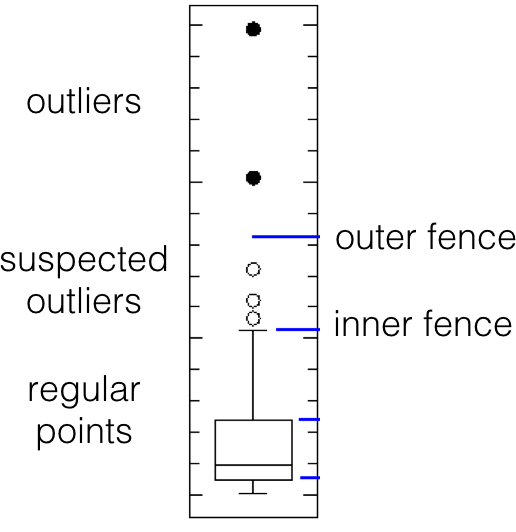
\includegraphics[height=0.8\textheight]{Images/boxplot_EN.png}
\\
Suspected outliers are marked by white disks, outliers by black disks.  \\ Use \texttt{boxplot()} and \texttt{boxplot.stats()} in \texttt{R} to plot and identify outliers in normally distributed data.
\end{center}
\newpage\ \\ \noindent The \textbf{Grubbs test} is another univariate test: 
$$H_0: \text{ no outlier in the data vs.\@ } H_1: \text{ \textbf{exactly one} outlier in the data.}$$

%, which takes into consideration the \textbf{number of observations} in the dataset:
\begin{itemize}
\item let $x_i$ be the value of feature $X$ for the $i^{\textrm{th}}$ unit, $1\leq i\leq N$,\item  let $(\overline{x},s_x)$ be the mean and standard deviation of feature $X$, 
\item let $\alpha$ be the desired significance level, and 
\item let  $T(\alpha/2N;N)$ be the critical value of the Student $t$-distribution. 
\end{itemize} 
The test statistic is $$G=\frac{\max_i\{|x_i-\overline{x}|\}}{s_x}=\frac{|x_{i^*}-\overline{x}|}{s_x}.$$

\newpage\ \\ \noindent Under $H_0$, $G$ follows a special distribution with critical value $$\ell(\alpha;N)=\frac{N-1}{\sqrt{N}}\sqrt{\frac{T^2(\alpha/2N,N)}{N-2+T^2(\alpha/2N,N)}}.$$ 
At significance level $\alpha$, we reject the null hypothesis in favour of the alternative (i.e.\@ $x_{i^*}$ is the outlier) if  $G\geq \ell(\alpha;N)$.
\newl If looking for more than one outlier, it can be tempting to classify every observation $i$ for which 
$$\frac{|x_i-\overline{x}|}{s_x} \geq \ell(\alpha;N)$$ as an outlier, but this is \textbf{NOT RECOMMENDED}. 
\newl Other generalizations are also problematic (cf.\@ outlier sequence). 

\newpage\ \\ \noindent Other common tests include:
\begin{itemize}

\item the \textbf{Mahalanobis distance}, which is linked to the leverage of an observation (a measure of influence), can also be used to find multi-dimen\-sio\-nal outliers, when all relationships are linear (or nearly linear);

\item the \textbf{Tietjen-Moore} test, which is used to find a specific number of outliers (this is similar to Grubbs' test, replacing $H_1$ by $H_k$);

\item the \textbf{generalized extreme studentized deviate} test, the preferred extension to Grubbs' test if the number of outliers is unknown; 

\item the \textbf{chi-square} test, when outliers affect the goodness-of-fit;

\item DBSCAN and other clustering-based outlier detection methods.

\end{itemize}



\fh{Visual Outlier Detection} 
\normalsize
\noindent The following simple examples illustrate the principles underlying \textbf{visual outlier and anomaly detection}. 

\noindent \textbf{Example 1:} on a specific day, the \textbf{height} of several plants in a nursery are measured. The records also show each plant's \textbf{age} (the number of weeks since the seed has been planted). 
\newl Very little can be said about the data at that stage: 
\begin{itemize}
\item the age of the plants (controlled by the nursery staff) seems to be somewhat haphazard, 
\item as does the response variable (height). 
\end{itemize}
\newpage\ 
\begin{center}
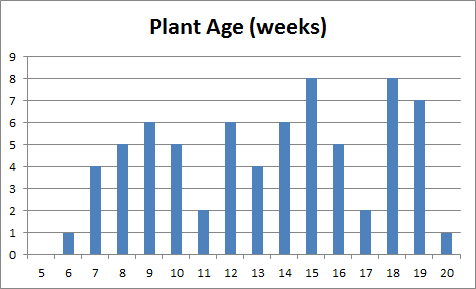
\includegraphics[width=0.47\textwidth]{Images/plant_age_EN}\\ 
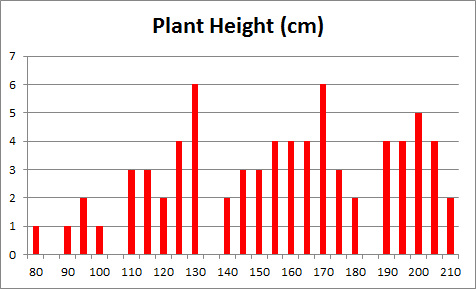
\includegraphics[width=0.47\textwidth]{Images/plant_height_EN}
\end{center}
\newpage\ \\ \noindent A scatter plot of the data reveals that \textbf{growth is strongly correlated with age} for the observations in the dataset; points clutter around a linear trend. \newl One point (in yellow) is easily identified as an \textbf{outlier}. \newl There are (at least) two possibilities: 
\begin{itemize}
\item either that measurement was botched or mis-entered in the database (representing an invalid entry), or 
\item that one specimen has experienced unusual growth (outlier).
\end{itemize}
Either way, the analyst has to investigate further.
\newpage\ 
\begin{center}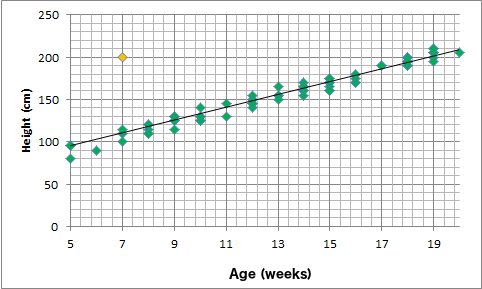
\includegraphics[width=0.90\textwidth]{Images/plant_height_vs_age_EN}\end{center} 
\newpage\ \\ \noindent \textbf{Example 2:} 
a government department has 11 service points. The monthly average arrival and service rates per teller for each service point are available. \newl The scatter plot of the service rate per teller ($y$ axis) against the arrival rate per teller ($x$ axis), with linear regression trend, is shown below. 

\begin{center}
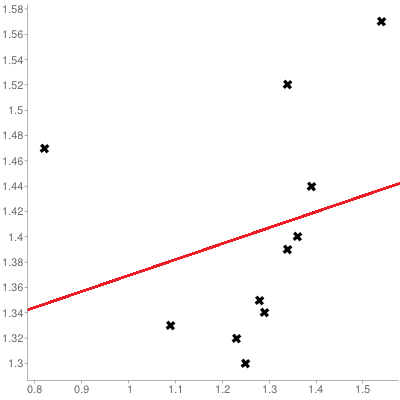
\includegraphics[width=0.37\textwidth]{Images/scatter_plot_linear_1}
\end{center}
\newpage\ \\ \noindent 
A similar chart, but with the left-most point removed from consideration, is shown below. 
\begin{center}
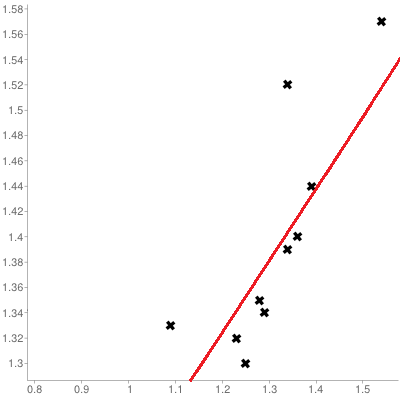
\includegraphics[width=0.37\textwidth]{Images/scatter_plot_linear_2}
\end{center}
The trend still slopes upward, but the fit is significantly improved. \newpage\ \\ \noindent This suggests that the removed observation is unduly \textbf{influential} (or anomalous) -- a better understanding of the relationship between arrivals and services is afforded if it is set aside. 
\newl Any attempt to fit that data point into the model must take this information into consideration. \newl The status of an influential observations \textbf{depends on the analysis that is ultimately conducted} -- a point may be influential for one analysis, but not for another. 
\newl Note that setting aside an influential observation does not mean that the observation is removed from the dataset -- only that it will not be used in a specific analysis. 
\newpage\ \\ \noindent \textbf{Example 3:} Measurements of the length of the appendage of a certain species of insect have been made on 71 individuals. Descriptive statistics have been computed; the results are shown below.
\begin{center}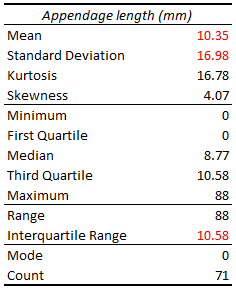
\includegraphics[height=0.72\textheight]{Images/appendage_length_descriptive_EN}
\end{center}  

\newpage\ \\ \noindent The descriptive statistics might help the analyst recognize the tell-tale signs that the distribution of appendage lengths is likely to: \begin{itemize}
\item be \textbf{asymmetrical} (since skewness is non-negligible), and
\item have a \textbf{``fat'' tail} (since large kurtosis, range $\gg$ interquartile range, and max $\gg Q_3$) \end{itemize} 
The mode, min, and $Q_1$ belong to individuals without appendages $\Longrightarrow$ at least two sub-groups in the population (perhaps split along the lines of juveniles/adults, or males/females).\newl Since max $\gg$ other observations, might it  belong to an \textbf{outlier}? The histogram of the measurements shows 3 individuals with long appendages.\newpage\ 
\begin{center} 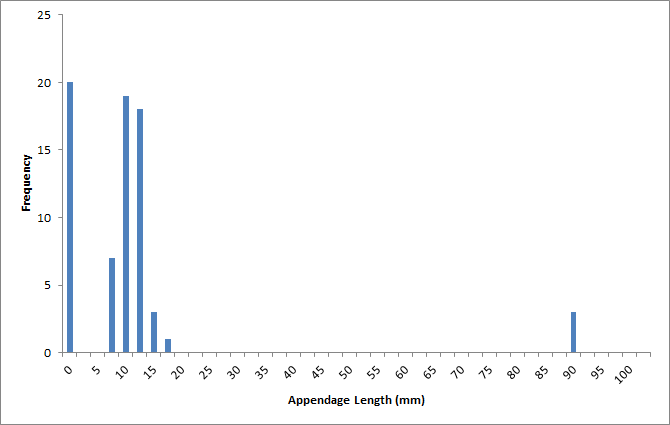
\includegraphics[width=0.9\textwidth]{Images/appendage_length_EN}
\end{center}  
\newpage \ \\ \noindent
It is plausible that these individuals belong to another species who were \textbf{erroneously added} to the dataset. \newl On its own, the chart does not constitute a proof of such an error, but it \textbf{raises the possibility of an error}, which is often the best that an analyst can do in the absence of subject matter expertise.
\newl This traditional approach to anomaly detection is difficult to apply to high-dimensional datasets because it is nearly impossible to visualize them directly $\Longrightarrow$ fundamentally different approaches are needed.\newl 
Dimension reduction methods can be used to provide a \textbf{low-dimensional representation} of the data on which to apply visual detection (see autoencoder example), but some information always gets lost in the process. 

\fh{6.1.1 -- Anomaly Detection as Statistical Learning} \label{6.1.1} 
\noindent Fraudulent behaviour is not always easily identifiable, even after the fact. \newl \textbf{Example:} credit card fraudsters try to disguise their transactions as regular and banal, and try to avoid outlandish behaviour. \newl Their goal: fool human observers into confusing  \textbf{plausible} (or possible) with \textbf{probable} (or at least, \textbf{not improbable}). \newl It is plausible that a generic 40-something father of 3 might purchase a new TV; is it probable that THIS particular father of 3  would do so? \newl But it's unlikely that a generic father of 3 who resides in North America would purchase a round of drinks at a dance club in Kiev. \newpage\ \\ \noindent Anomaly detection is really a problem in \textbf{applied probability}. Let $I$ be what is known about the dataset/situation: 
\begin{itemize}
\item behaviour of individual observations,
\item behaviour of observations as a whole, 
\item anomalous/normal verdict for a number of similar observations, etc.
\end{itemize} \textbf{Main Question:} is $P(\text{obs.\@ is anomalous}\mid I) > P(\text{obs.\@ is normal}\mid I)?$ 
\newl Anomaly detection models assume \textbf{stationarity of regular observations}: that the underlying mechanism that generates regular data does not change much over time.\newpage \ \\ \noindent For time series data, this means that it may be necessary to first perform \textbf{trend and seasonality extraction}.\newl 
\textbf{Example:} supply chains play a crucial role in the transportation of goods from one part of the world to another -- as the saying goes, ``a given chain is only as strong as its weakest link.'' \newl Say that marine cargo departing Shanghai in Feb'13 took two more days, on average, to arrive in Vancouver than those departing in Jul'17.
\begin{itemize}
\item Has the shipping process  improved in the intervening years? 
\item Do departures in Feb usually take longer to reach Vancouver? 
\item Are either the Feb'13 or the Jul'17 performance anomalous?
\end{itemize} \newpage\ \\ \noindent Seasonal variability is relevant to supply chain monitoring: quantifying and accounting for impact severity is of great interest. \newl  
\textbf{Potential Solution:} create an \textbf{index} to track container transit times. \newl This index should depict 
\begin{itemize}
\item \textbf{reliability} and
\item \textbf{variability} of transit times, 
\item and allow for performance comparison between differing time periods.
\end{itemize} 
\newpage\ \\ \noindent Consider the scenario where we want to compare the  monthly performance, irrespective of the transit season, of the corridor $$\textbf{Shanghai} \to \textbf{Port Metro Vancouver/Prince Rupert} \to \textbf{Toronto}.$$  
\begin{center}
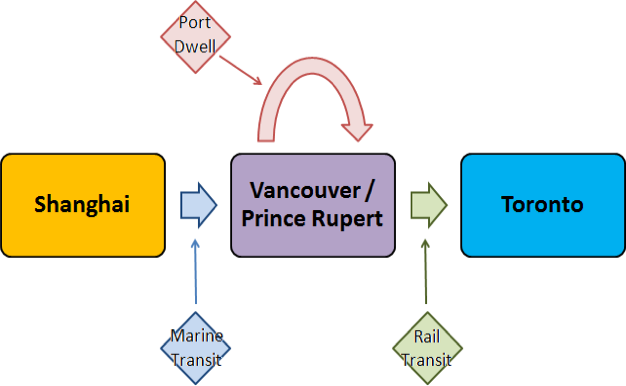
\includegraphics[width=0.65\textwidth]{Images/mmsc_EN.png}
\end{center}
\newpage\ \\ \noindent 
For each of the three segments (Marine Transit, Port Dwell, Rail Transit), the data consists of:
\begin{itemize}
\item monthly empirical distribution of transit/dwell times
\item built from sub-samples (assumed to be randomly selected and fully representative) of all containers entering the appropriate segment.
\end{itemize}
Specific containers are not followed from Shanghai to Toronto: no covariance information about the various transit/dwell times is available. \newl Each segment's performance is measured using \textbf{fluidity indicators}, which are computed using various statistics of the transit/dwell time distributions for each of the supply chain segments. 
\newpage\ \begin{description} 
\item[Reliability Indicator (RI)] -- the ratio of the 95$^{\text{th}}$ percentile to the 5$^{\text{th}}$ percentile of transit/dwell times. \par A high RI indicates high volatility, whereas a low RI $(\approx 1)$ indicates a reliable corridor.
\item[Buffer Index (BI)] -- the ratio of the positive difference between the 95$^{\text{th}}$ percentile and the mean, to the mean. \par A small BI $(\approx 0)$ indicates only slight variability in the upper (longer) transit/dwell times; a large BI indicates that the variability of the longer transit/dwell times is high, and that outliers might be found there;
\item[Coefficient of Variation (CV)] -- the ratio of the standard deviation of transit/dwell times to the mean transit/dwell time.  
\end{description}
\newpage\ \\ 
\begin{center}
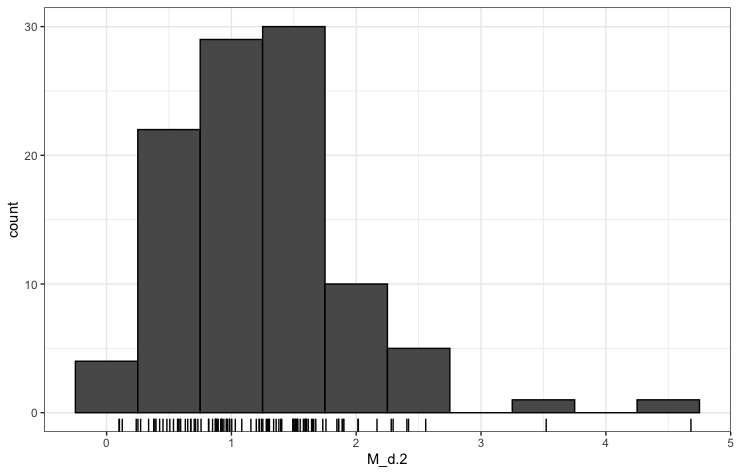
\includegraphics[width=\textwidth]{Images/Rplot}
\\
%\begin{threeparttable}
 \setlength{\tabcolsep}{1pt}
\begin{tabularx}{\textwidth}{p{0.1\textwidth} p{0.1\textwidth} p{0.1\textwidth} p{0.1\textwidth} p{0.1\textwidth} p{0.1\textwidth} p{0.1\textwidth} p{0.1\textwidth} p{0.1\textwidth}}


\hhline{}
\arrayrulecolor{black}

\multicolumn{1}{!{\huxvb{0, 0, 0}{0}}p{0.1\textwidth}!{\huxvb{0, 0, 0}{0}}}{\hspace{0pt}\parbox[b]{0.1\textwidth-10pt-10pt}{\huxtpad{6pt + 1em}\raggedright \textbf{Segmt}\huxbpad{6pt}}} &
\multicolumn{1}{p{0.1\textwidth}!{\huxvb{0, 0, 0}{0}}}{\hspace{10pt}\parbox[b]{0.1\textwidth-10pt-10pt}{\huxtpad{6pt + 1em}\raggedleft \textbf{Freq}\huxbpad{6pt}}} &
\multicolumn{1}{p{0.1\textwidth}!{\huxvb{0, 0, 0}{0}}}{\hspace{10pt}\parbox[b]{0.1\textwidth-10pt-10pt}{\huxtpad{6pt + 1em}\raggedleft \textbf{Mean}\huxbpad{6pt}}} &
\multicolumn{1}{p{0.1\textwidth}!{\huxvb{0, 0, 0}{0}}}{\hspace{10pt}\parbox[b]{0.1\textwidth-10pt-10pt}{\huxtpad{6pt + 1em}\raggedleft \textbf{SD}\huxbpad{6pt}}} &
\multicolumn{1}{p{0.1\textwidth}!{\huxvb{0, 0, 0}{0}}}{\hspace{10pt}\parbox[b]{0.1\textwidth-10pt-10pt}{\huxtpad{6pt + 1em}\raggedleft \textbf{C05}\huxbpad{6pt}}} &
\multicolumn{1}{p{0.1\textwidth}!{\huxvb{0, 0, 0}{0}}}{\hspace{10pt}\parbox[b]{0.1\textwidth-10pt-10pt}{\huxtpad{6pt + 1em}\raggedleft \textbf{C95}\huxbpad{6pt}}} &
\multicolumn{1}{p{0.1\textwidth}!{\huxvb{0, 0, 0}{0}}}{\hspace{10pt}\parbox[b]{0.1\textwidth-10pt-10pt}{\huxtpad{6pt + 1em}\raggedleft \textbf{RI}\huxbpad{6pt}}} &
\multicolumn{1}{p{0.1\textwidth}!{\huxvb{0, 0, 0}{0}}}{\hspace{10pt}\parbox[b]{0.1\textwidth-10pt-10pt}{\huxtpad{6pt + 1em}\raggedleft \textbf{BI}\huxbpad{6pt}}} &
\multicolumn{1}{p{0.1\textwidth}!{\huxvb{0, 0, 0}{0}}}{\hspace{10pt}\parbox[b]{0.1\textwidth-10pt-10pt}{\huxtpad{6pt + 1em}\raggedleft \textbf{CV}\huxbpad{6pt}}} \tabularnewline[-0.5pt]


\hhline{>{\huxb{0, 0, 0}{0.4}}->{\huxb{0, 0, 0}{0.4}}->{\huxb{0, 0, 0}{0.4}}->{\huxb{0, 0, 0}{0.4}}->{\huxb{0, 0, 0}{0.4}}->{\huxb{0, 0, 0}{0.4}}->{\huxb{0, 0, 0}{0.4}}->{\huxb{0, 0, 0}{0.4}}->{\huxb{0, 0, 0}{0.4}}-}
\arrayrulecolor{black}

\multicolumn{1}{!{\huxvb{0, 0, 0}{0}}p{0.1\textwidth}!{\huxvb{0, 0, 0}{0}}}{\hspace{10pt}\parbox[b]{0.1\textwidth-10pt-10pt}{\huxtpad{6pt + 1em}\raggedright $A$\huxbpad{6pt}}} &
\multicolumn{1}{p{0.1\textwidth}!{\huxvb{0, 0, 0}{0}}}{\hspace{10pt}\parbox[b]{0.1\textwidth-10pt-10pt}{\huxtpad{6pt + 1em}\raggedleft 3286\huxbpad{6pt}}} &
\multicolumn{1}{p{0.1\textwidth}!{\huxvb{0, 0, 0}{0}}}{\hspace{10pt}\parbox[b]{0.1\textwidth-10pt-10pt}{\huxtpad{6pt + 1em}\raggedleft 12.10\huxbpad{6pt}}} &
\multicolumn{1}{p{0.1\textwidth}!{\huxvb{0, 0, 0}{0}}}{\hspace{10pt}\parbox[b]{0.1\textwidth-10pt-10pt}{\huxtpad{6pt + 1em}\raggedleft 3.33\huxbpad{6pt}}} &
\multicolumn{1}{p{0.1\textwidth}!{\huxvb{0, 0, 0}{0}}}{\hspace{10pt}\parbox[b]{0.1\textwidth-10pt-10pt}{\huxtpad{6pt + 1em}\raggedleft 7.06\huxbpad{6pt}}} &
\multicolumn{1}{p{0.1\textwidth}!{\huxvb{0, 0, 0}{0}}}{\hspace{10pt}\parbox[b]{0.1\textwidth-10pt-10pt}{\huxtpad{6pt + 1em}\raggedleft 17.00\huxbpad{6pt}}} &
\multicolumn{1}{p{0.1\textwidth}!{\huxvb{0, 0, 0}{0}}}{\hspace{10pt}\parbox[b]{0.1\textwidth-10pt-10pt}{\huxtpad{6pt + 1em}\raggedleft 2.41\huxbpad{6pt}}} &
\multicolumn{1}{p{0.1\textwidth}!{\huxvb{0, 0, 0}{0}}}{\hspace{10pt}\parbox[b]{0.1\textwidth-10pt-10pt}{\huxtpad{6pt + 1em}\raggedleft 0.41\huxbpad{6pt}}} &
\multicolumn{1}{p{0.1\textwidth}!{\huxvb{0, 0, 0}{0}}}{\hspace{10pt}\parbox[b]{0.1\textwidth-10pt-10pt}{\huxtpad{6pt + 1em}\raggedleft 0.27\huxbpad{6pt}}} \tabularnewline[-0.5pt]


\hhline{}
\arrayrulecolor{black}

\multicolumn{1}{!{\huxvb{0, 0, 0}{0}}p{0.1\textwidth}!{\huxvb{0, 0, 0}{0}}}{\hspace{10pt}\parbox[b]{0.1\textwidth-10pt-10pt}{\huxtpad{6pt + 1em}\raggedright $B$\huxbpad{6pt}}} &
\multicolumn{1}{p{0.1\textwidth}!{\huxvb{0, 0, 0}{0}}}{\hspace{10pt}\parbox[b]{0.1\textwidth-10pt-10pt}{\huxtpad{6pt + 1em}\raggedleft 2594\huxbpad{6pt}}} &
\multicolumn{1}{p{0.1\textwidth}!{\huxvb{0, 0, 0}{0}}}{\hspace{10pt}\parbox[b]{0.1\textwidth-10pt-10pt}{\huxtpad{6pt + 1em}\raggedleft 10.09\huxbpad{6pt}}} &
\multicolumn{1}{p{0.1\textwidth}!{\huxvb{0, 0, 0}{0}}}{\hspace{10pt}\parbox[b]{0.1\textwidth-10pt-10pt}{\huxtpad{6pt + 1em}\raggedleft 4.43\huxbpad{6pt}}} &
\multicolumn{1}{p{0.1\textwidth}!{\huxvb{0, 0, 0}{0}}}{\hspace{10pt}\parbox[b]{0.1\textwidth-10pt-10pt}{\huxtpad{6pt + 1em}\raggedleft 3.88\huxbpad{6pt}}} &
\multicolumn{1}{p{0.1\textwidth}!{\huxvb{0, 0, 0}{0}}}{\hspace{10pt}\parbox[b]{0.1\textwidth-10pt-10pt}{\huxtpad{6pt + 1em}\raggedleft 18.20\huxbpad{6pt}}} &
\multicolumn{1}{p{0.1\textwidth}!{\huxvb{0, 0, 0}{0}}}{\hspace{10pt}\parbox[b]{0.1\textwidth-10pt-10pt}{\huxtpad{6pt + 1em}\raggedleft 4.69\huxbpad{6pt}}} &
\multicolumn{1}{p{0.1\textwidth}!{\huxvb{0, 0, 0}{0}}}{\hspace{10pt}\parbox[b]{0.1\textwidth-10pt-10pt}{\huxtpad{6pt + 1em}\raggedleft 0.80\huxbpad{6pt}}} &
\multicolumn{1}{p{0.1\textwidth}!{\huxvb{0, 0, 0}{0}}}{\hspace{10pt}\parbox[b]{0.1\textwidth-10pt-10pt}{\huxtpad{6pt + 1em}\raggedleft 0.44\huxbpad{6pt}}} \tabularnewline[-0.5pt]


\hhline{}
\arrayrulecolor{black}

\multicolumn{1}{!{\huxvb{0, 0, 0}{0}}p{0.1\textwidth}!{\huxvb{0, 0, 0}{0}}}{\hspace{10pt}\parbox[b]{0.1\textwidth-10pt-10pt}{\huxtpad{6pt + 1em}\raggedright $C$\huxbpad{6pt}}} &
\multicolumn{1}{p{0.1\textwidth}!{\huxvb{0, 0, 0}{0}}}{\hspace{10pt}\parbox[b]{0.1\textwidth-10pt-10pt}{\huxtpad{6pt + 1em}\raggedleft 2142\huxbpad{6pt}}} &
\multicolumn{1}{p{0.1\textwidth}!{\huxvb{0, 0, 0}{0}}}{\hspace{10pt}\parbox[b]{0.1\textwidth-10pt-10pt}{\huxtpad{6pt + 1em}\raggedleft 5.96\huxbpad{6pt}}} &
\multicolumn{1}{p{0.1\textwidth}!{\huxvb{0, 0, 0}{0}}}{\hspace{10pt}\parbox[b]{0.1\textwidth-10pt-10pt}{\huxtpad{6pt + 1em}\raggedleft 5.08\huxbpad{6pt}}} &
\multicolumn{1}{p{0.1\textwidth}!{\huxvb{0, 0, 0}{0}}}{\hspace{10pt}\parbox[b]{0.1\textwidth-10pt-10pt}{\huxtpad{6pt + 1em}\raggedleft 0.19\huxbpad{6pt}}} &
\multicolumn{1}{p{0.1\textwidth}!{\huxvb{0, 0, 0}{0}}}{\hspace{10pt}\parbox[b]{0.1\textwidth-10pt-10pt}{\huxtpad{6pt + 1em}\raggedleft 14.40\huxbpad{6pt}}} &
\multicolumn{1}{p{0.1\textwidth}!{\huxvb{0, 0, 0}{0}}}{\hspace{10pt}\parbox[b]{0.1\textwidth-10pt-10pt}{\huxtpad{6pt + 1em}\raggedleft 77.12\huxbpad{6pt}}} &
\multicolumn{1}{p{0.1\textwidth}!{\huxvb{0, 0, 0}{0}}}{\hspace{10pt}\parbox[b]{0.1\textwidth-10pt-10pt}{\huxtpad{6pt + 1em}\raggedleft 1.41\huxbpad{6pt}}} &
\multicolumn{1}{p{0.1\textwidth}!{\huxvb{0, 0, 0}{0}}}{\hspace{10pt}\parbox[b]{0.1\textwidth-10pt-10pt}{\huxtpad{6pt + 1em}\raggedleft 0.85\huxbpad{6pt}}} \tabularnewline[-0.5pt]


\hhline{}
\arrayrulecolor{black}
\end{tabularx} \end{center}
\newpage\ \\ \noindent The time series of monthly fluidity indicators  are then \textbf{decomposed} into: 
\begin{itemize} 
\item trend $\Longrightarrow$ \textbf{expected behaviour}
\item seasonal component (seasonality, trading-day, moving-holiday) $\Longrightarrow$ \textbf{expected behaviour} 
\item structural breaks, $\Longrightarrow$ \textbf{explained unexpected behaviour} and 
\item irregular component $\Longrightarrow$ chain \textbf{volatility}
\end{itemize}
A high irregular component at a given time indicates a poor performance against expectations $\Longrightarrow$ an \textbf{anomalous observation}.  
\newpage
\begin{center}
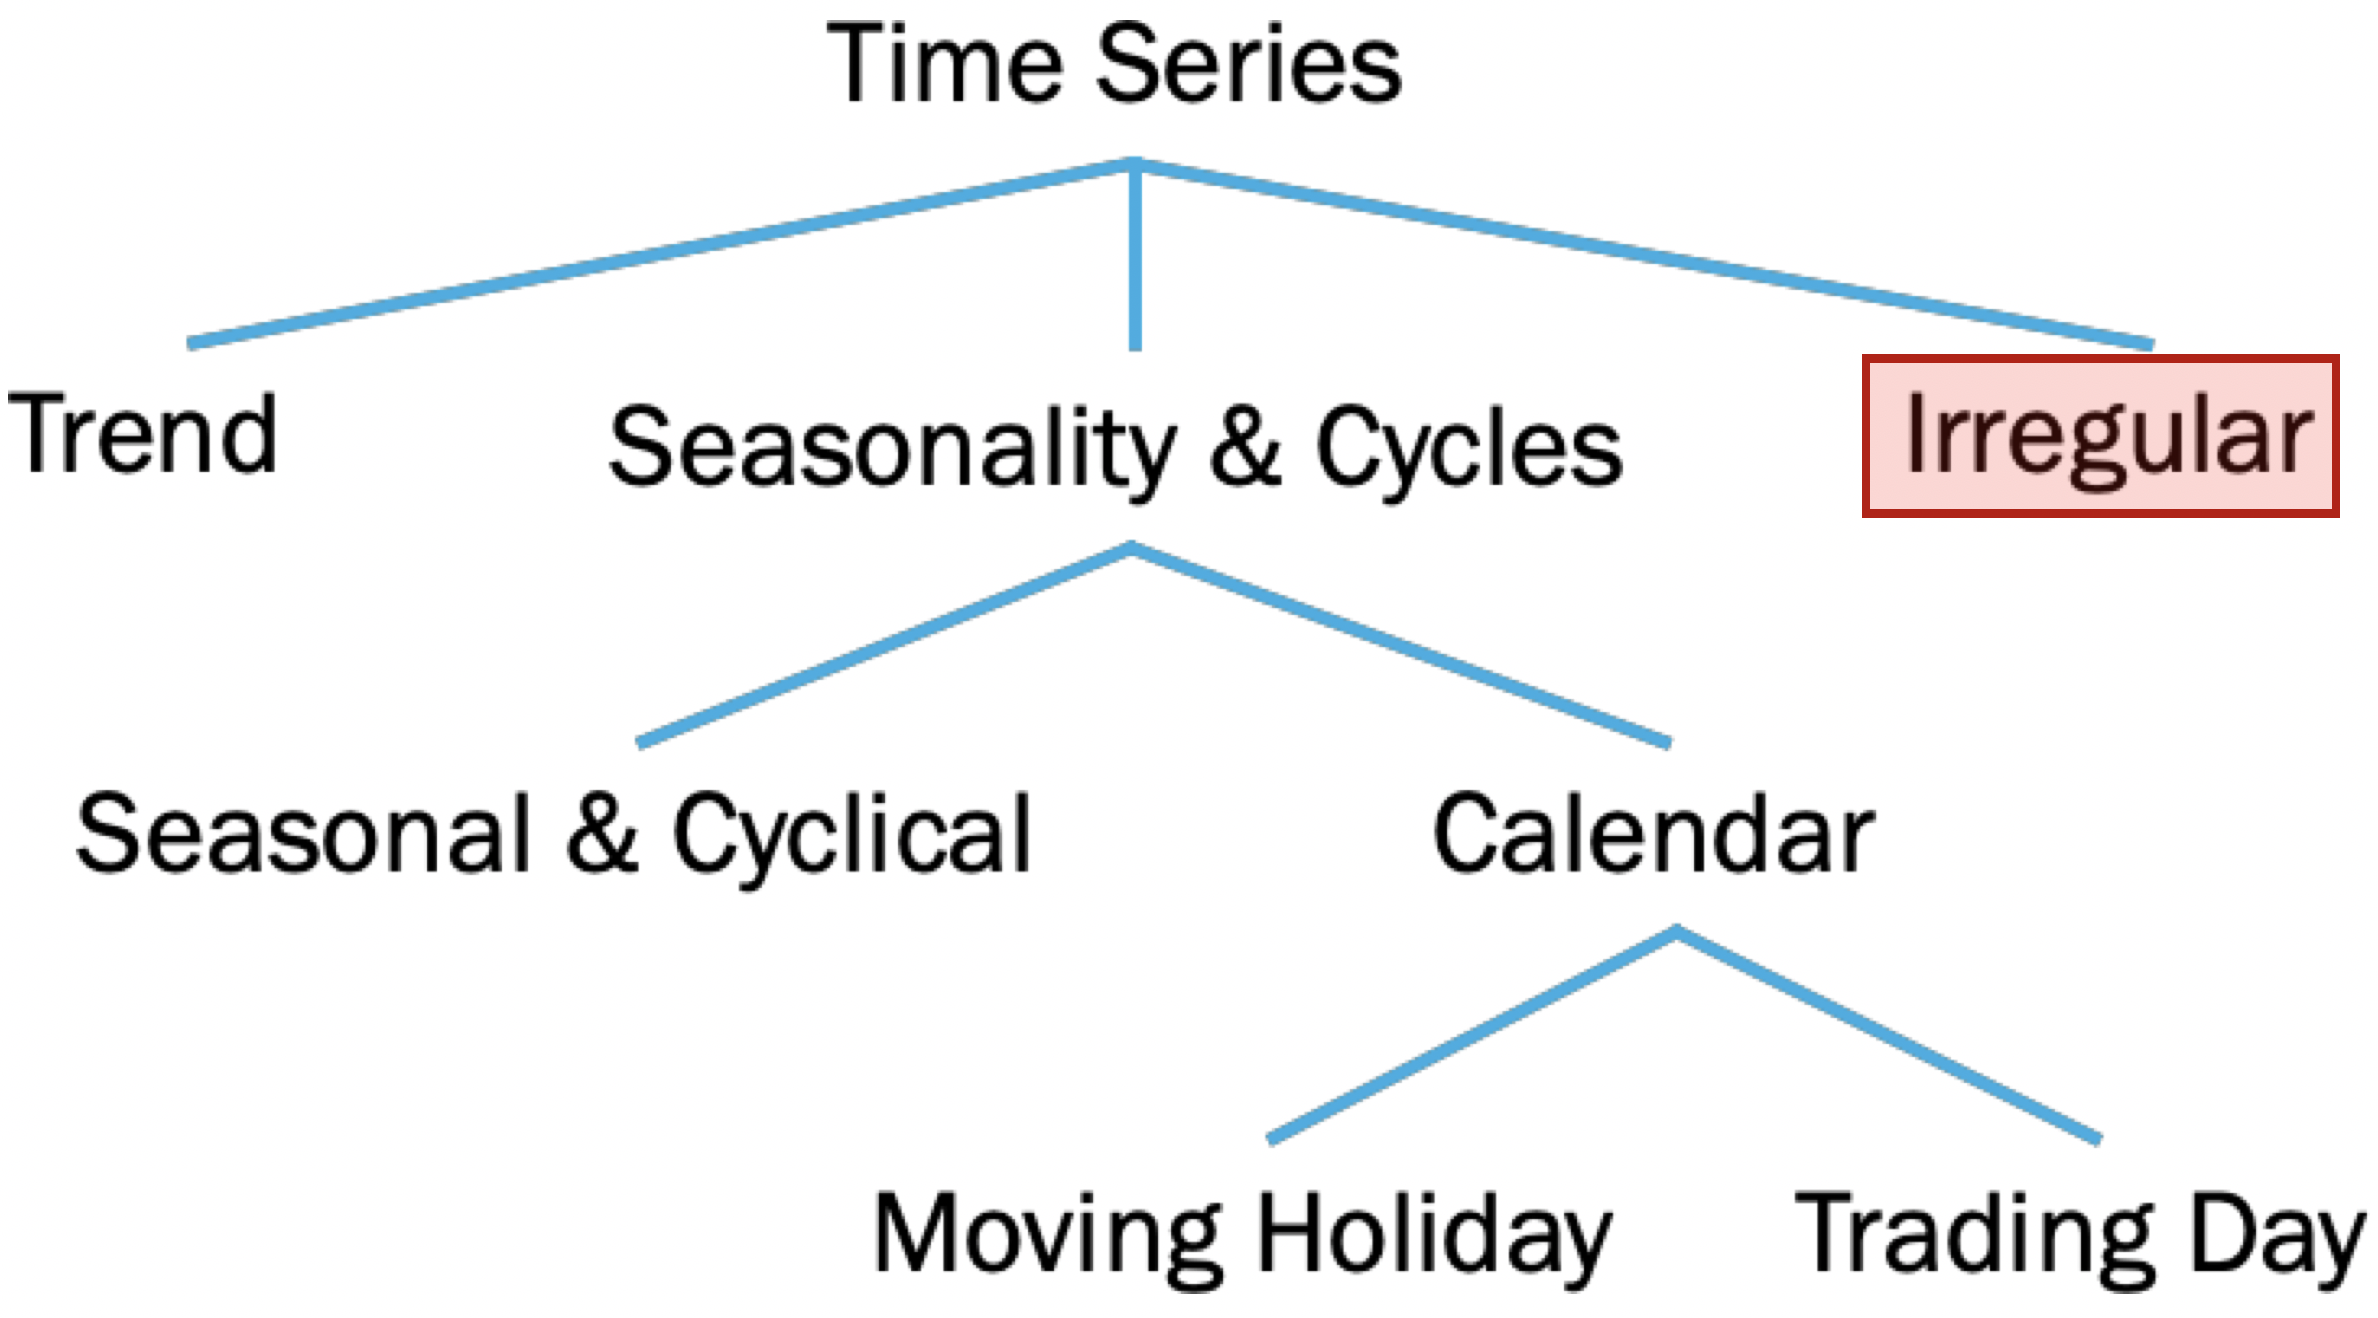
\includegraphics[width=0.85\textwidth]{Images/decomposition_EN.png} \end{center} 
Conceptual time series decomposition (after structural breaks are removed); potential anomalous behaviour should be searched for in the \textbf{irregular component}.
\newpage\ \\ \noindent In general, the decomposition follows a model which is 
\begin{itemize} 
\item multiplicative;
\item additive, or 
\item pseudo-additive.
\end{itemize}
The choice of a model is driven by data behaviour and choice of assumptions; the X12 model automates some of the aspects of the decomposition, but manual intervention and diagnostics are still required.\newl
\textbf{IMPORTANT NOTE:} anomaly detection often requires modeling choices/ assumptions. 
\newpage\ \\ \noindent 
The \textbf{additive model}, for instance, assumes that: 
\begin{enumerate} \item the seasonal component $S_t$ and the irregular component $I_t$ are independent of the trend $T_t$; \item  the seasonal component $S_t$ remains stable from year to year; and \item there is no seasonal fluctuation: $\sum_{j=1}^{12} S_{t+j}=0 $.\end{enumerate} 
Mathematically, the model is expressed as:
    \begin{equation*}
        O_t = T_t + S_t + I_t
    \end{equation*}
    All components share the same dimensions and units. \newpage\ \\ \noindent After seasonality adjustment,the seasonality adjusted series is:
    \begin{equation*}
        SA_t = O_t - S_t = T_t + I_t
    \end{equation*}
The multiplicative and pseudo-additive models are defined in similar ways:\begin{itemize} 
\item if the size of $S_t$   increases/decreases over time, use s multiplicative model; 
\item otherwise, use an additive model.
\end{itemize}
The data decomposition/preparation process is illustrated with the 40-month time series of marine transit CVs from 2010-2013. \newl The size of the peaks and troughs seems fairly constant with respect to the changing trend $\Longrightarrow$ use the additive model.
\newpage\ \begin{center}
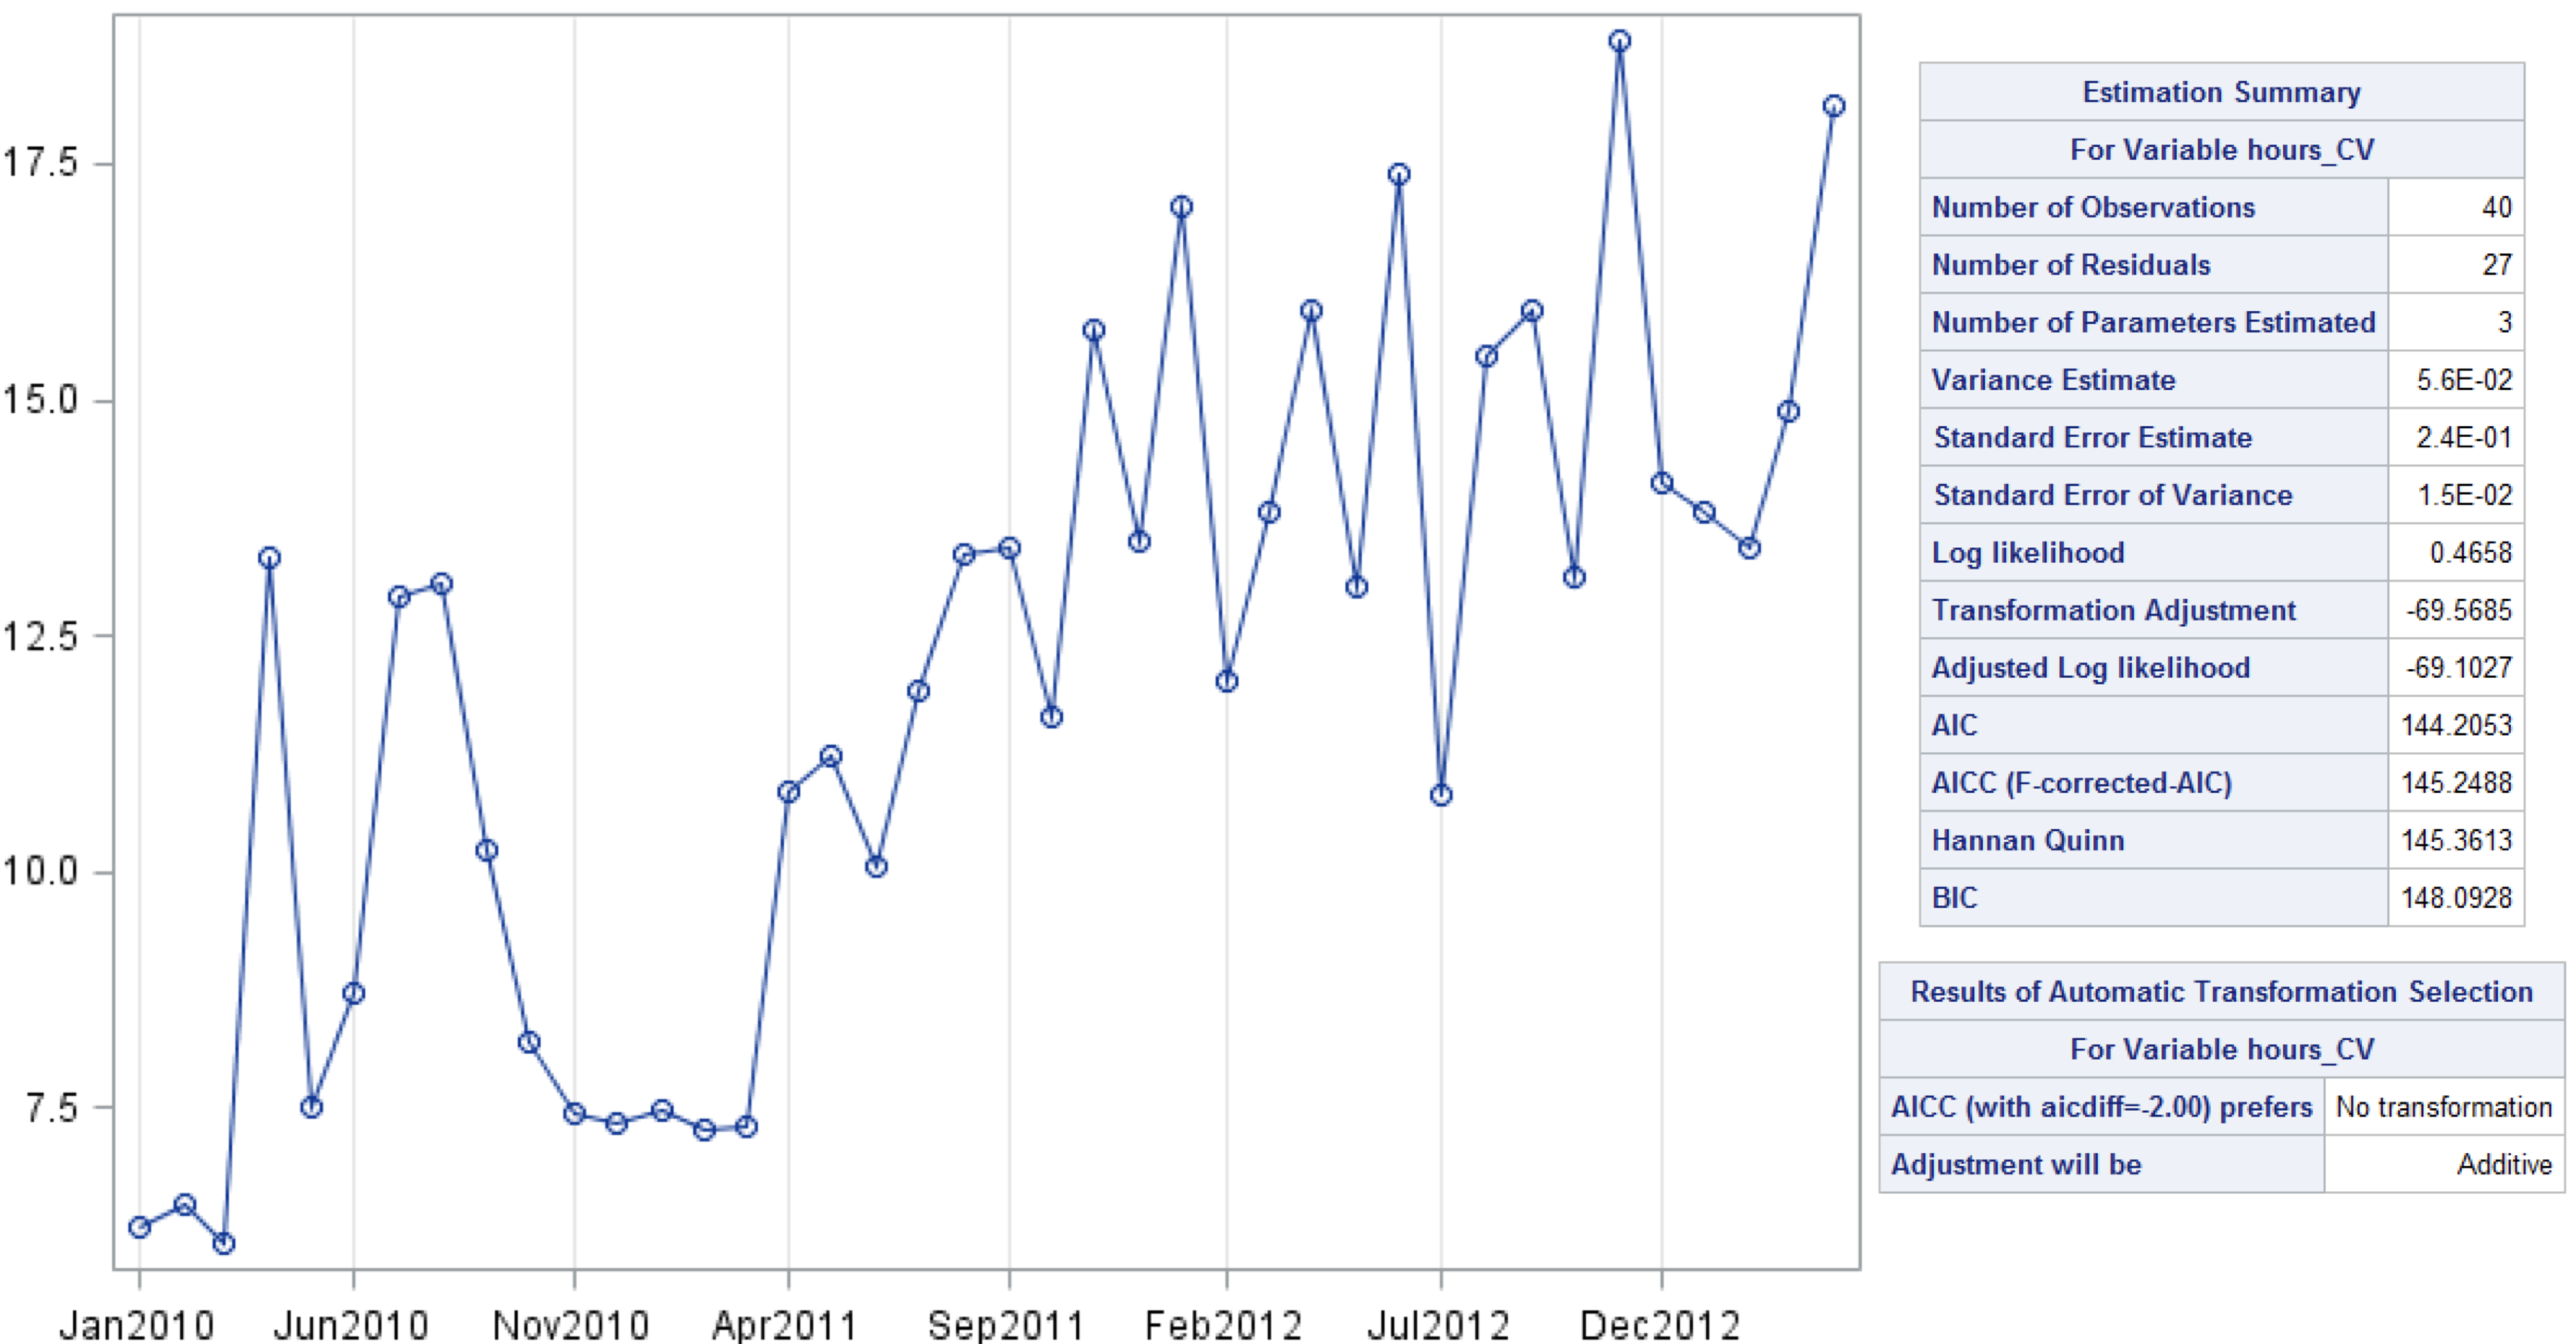
\includegraphics[width=\textwidth]{Images/CV_continuously.png}
\end{center}\newpage \ \\ \noindent A structural break (trend level shift) is identified at OCT2010. \newl The SI (Seasonal Irregular) chart shows that there are more than one irregular component which exhibits volatility.
\begin{center}
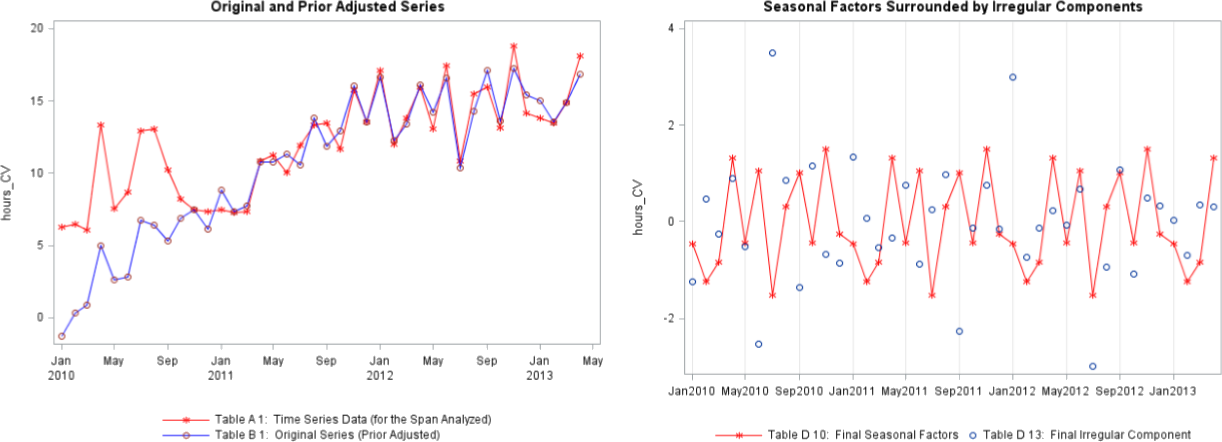
\includegraphics[width=\textwidth]{Images/DiffComponents.png}
\end{center}
\newpage \ \\ \noindent The adjusted series is shown below; the trend and irregular components are also shown separately for readability. \newl It is on the irregular component that detection anomaly would be conducted. 
\begin{center}
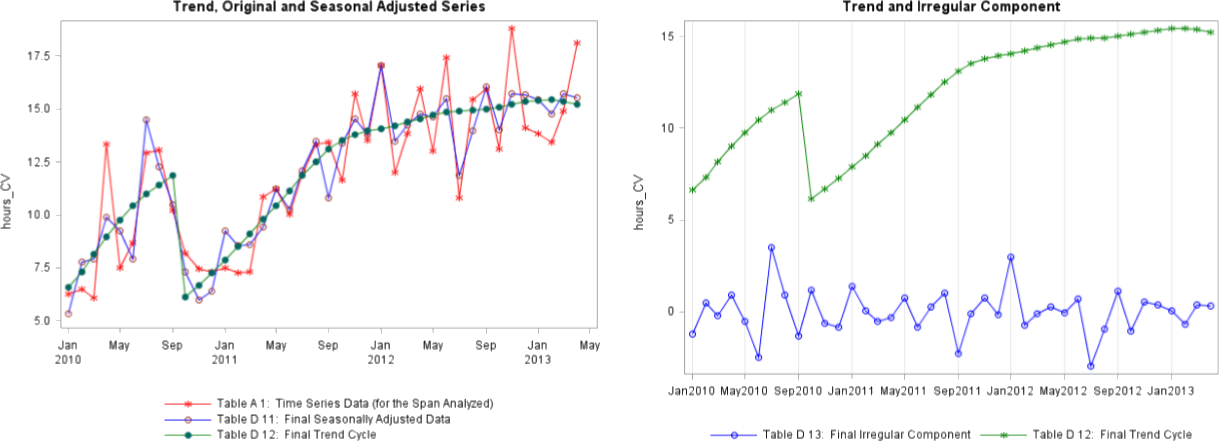
\includegraphics[width=\textwidth]{Images/adjustedplot.png}\end{center} 
\newpage\ \\ \noindent Given that the vast majority of observations in a general problem are typically ``normal'', another conceptually important approach is to view anomaly detection as a:
\begin{itemize}
\item \textbf{rare occurrence learning} classification problem, or \item  \textbf{novelty detection} data stream problem. \end{itemize} 
While there a number of strategies that use regular classification/clustering algorithms for anomaly detection, they are rarely successful unless they are \textbf{adapted} or \textbf{modified for the anomaly detection context}.
\newl \textbf{MORAL OF THE STORY:} anomaly detection is a difficult problem.
\fh{Basic Concepts}
\noindent Generic systems (think of the monthly transit/dwell times from supply chains) may be realized in 
\begin{itemize}
\item \textbf{normal} states, or  \item \textbf{abnormal} states. 
\end{itemize} 
Normality is not confined to finding the most likely state -- infrequently occurring states could still be normal or plausible under some interpretation of the system. \newpage\ \\ \noindent A system's states are the results of processes or behaviours that follow certain \textbf{natural rules} and \textbf{broad principles}; the observations are a manifestation of these states. \newl Data allows for inferences to be made about the underlying processes, which can be tested or invalidated by the collection of additional data. 
\newl When the inputs are perturbed, the corresponding outputs are likely to be perturbed as well. \newl If anomalies arise from perturbed processes, the \textbf{anomaly detection problem} could be helped along by being able to identify when the underlying process is abnormal. 
\newpage\ \\ \noindent  \textbf{Supervised} anomaly detection algorithms require a \begin{enumerate}
\item \textbf{training set of historical labeled data} on which to build the prediction model (usually costly to obtain), and 
\item testing set on which to evaluate the model's performance in terms of 
\begin{itemize}
\item \textbf{True Positives} ($\text{TP}$)  -- detected anomalies that actually arise from process abnormalities; 
\item \textbf{True Negatives} ($\text{TN}$)  -- predicted normal observations that indeed arise from normal processes; 
\item \textbf{False Positives} ($\text{FP}$)  -- detected anomalies corresponding to regular processes, and 
\item \textbf{False Negatives} ($\text{FN}$) -- predicted normal observations that are in fact the product of an abnormal process.
\end{itemize}
\end{enumerate}
\newpage\ \\ \noindent This is often summarized in a \textbf{confusion matrix}:
\begin{center}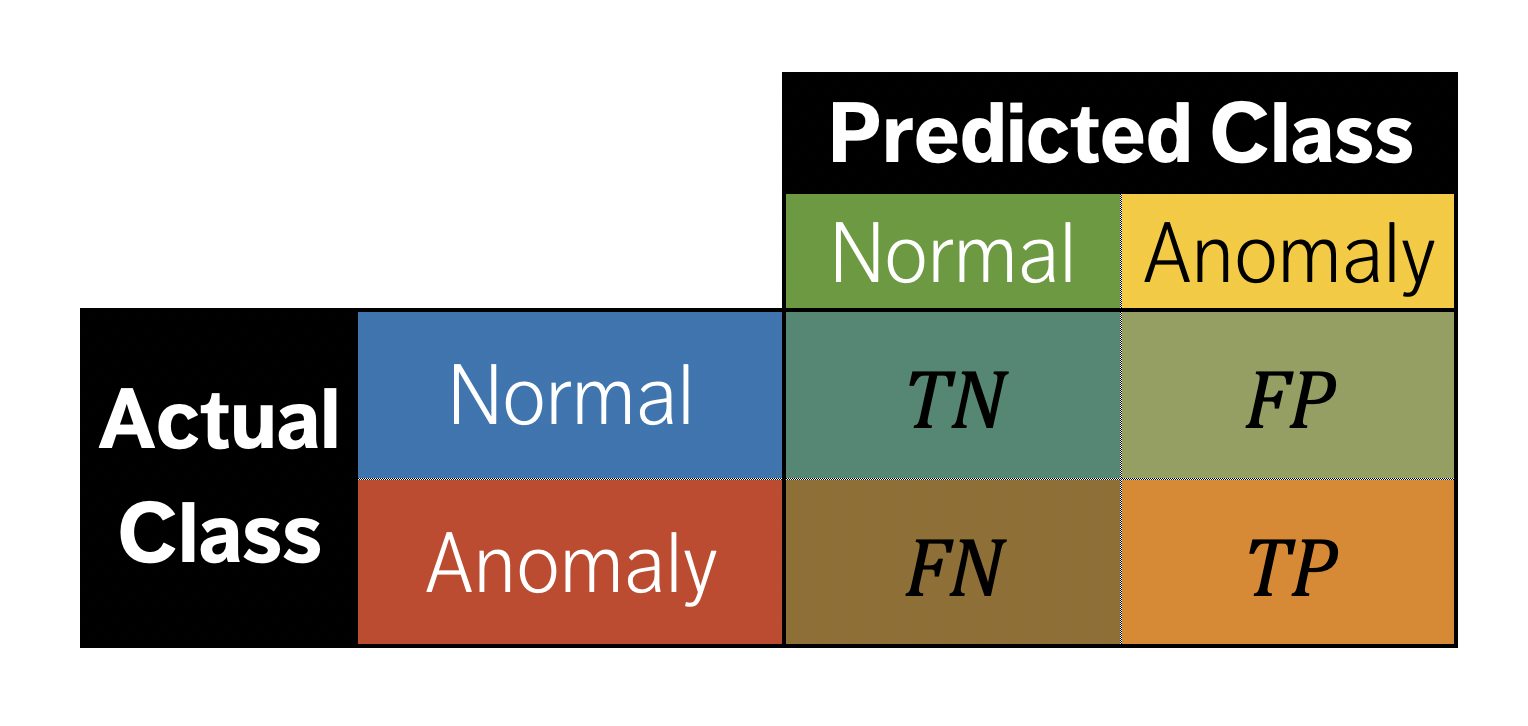
\includegraphics[width=0.6\textwidth]{Images/Confusion_EN.png}\end{center}
Na\"{\i}vely, one might look for an algorithm which maximizes the \textbf{accuracy} $$a=\frac{\text{TN}+\text{TP}}{\text{TN}+\text{TP}+\text{FN}+\text{FP}}.$$ For rare occurrences, this is a losing strategy (see weapon smuggling ex.). \newpage\ \\ \noindent \textbf{Better approach:} try to minimize the FP rate and the FN rate under the assumption that the \textbf{cost of making a false negative error could be substantially higher than the cost of making a false positive error}. \newl 
For a testing set with $d=\text{FN}+\text{TP}$ \textbf{true outliers}, assume that an anomaly detection algorithm identifies $m=\text{FP}+\text{TP}$ \textbf{suspicious observations}, of which $n=\text{TP}$ are \textbf{known} to be true outliers. \newl How well did the algorithm \textbf{perform}?   
\begin{description}
\item[Precision:] proportion of true outliers among suspicious observations $$p=\frac{n}{m}=\frac{\text{TP}}{\text{FP}+\text{TP}};$$ if most of the suspicious points are true outliers, $p\approx 1$;
\newpage\ \item[Recall:] proportion of true outliers detected by the algorithm
$$r=\frac{n}{d}=\frac{\text{TP}}{\text{FN}+\text{TP}};$$ if most of the true outliers are identified by the algorithm, $r\approx 1$;
\item[$F_1-$Score:] harmonic mean of the algorithm's precision and its recall on the testing set 
$$F_1=\frac{2pr}{p+r}=\frac{2\text{TP}}{2\text{TP}+\text{FP}+\text{FN}}.$$
\end{description}
\textbf{Question:} precision, recall, and $F_1-$score do not incorporate $\text{TN}$ in the evaluation process. Is this likely to be a problem? 
\newpage\ \\ \noindent \textbf{Example:} consider a test dataset with $5000$ observations, $100$ of which are anomalous.\newl An algorithm that predicts all observations to be anomalous yields 
\begin{center}
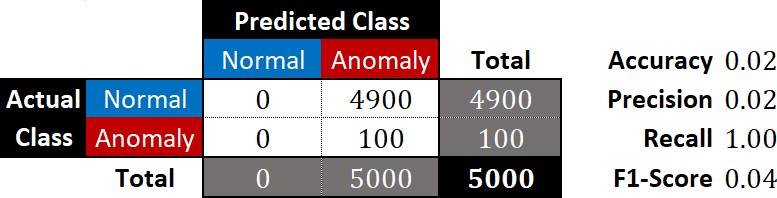
\includegraphics[width=\textwidth]{Images/Ex1.png}
\end{center}
\newpage\ \\ \noindent An algorithm that only detects $10$ of the true outliers and $x$ of the normal observations yields
\begin{center}
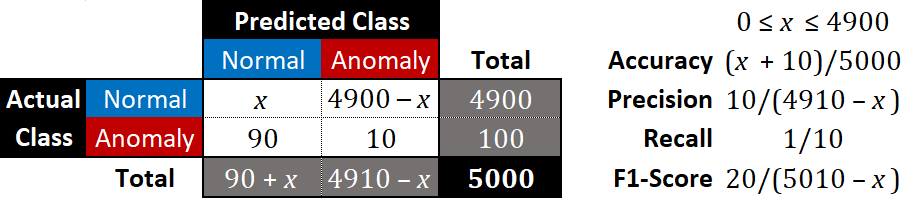
\includegraphics[width=\textwidth]{Images/Ex2.png}\\ \ \\ 
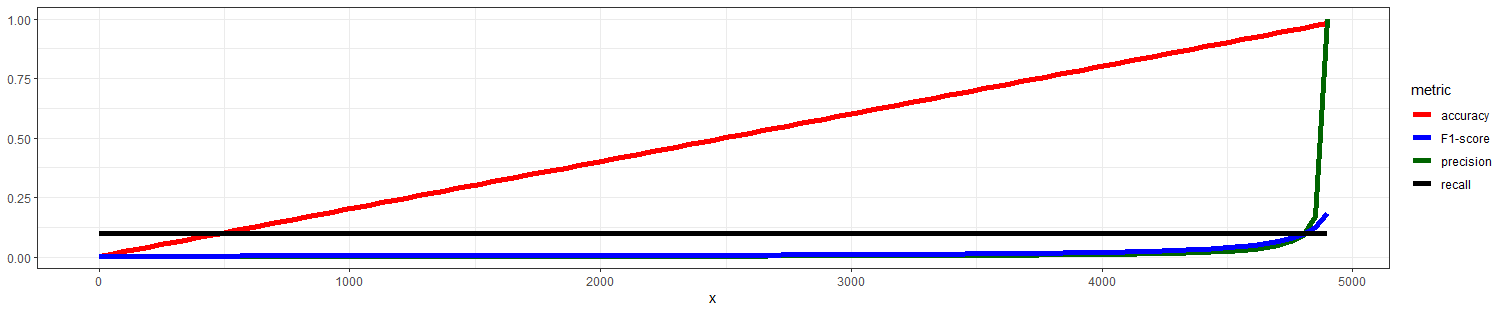
\includegraphics[width=\textwidth]{Images/AODA_metrics.png}
\end{center}
\newpage \ \\ \noindent SL algorithms include: 
\begin{itemize}
\item logistic regression
\item na\"{\i}ve or optimal Bayes classifiers
\item support vector machines
\item neural networks (deep learning)
\item decision trees, etc.
\end{itemize}
Such algorithms incorporate (and help us learn) historical patterns and rules. 
\newpage\ 
\begin{center}
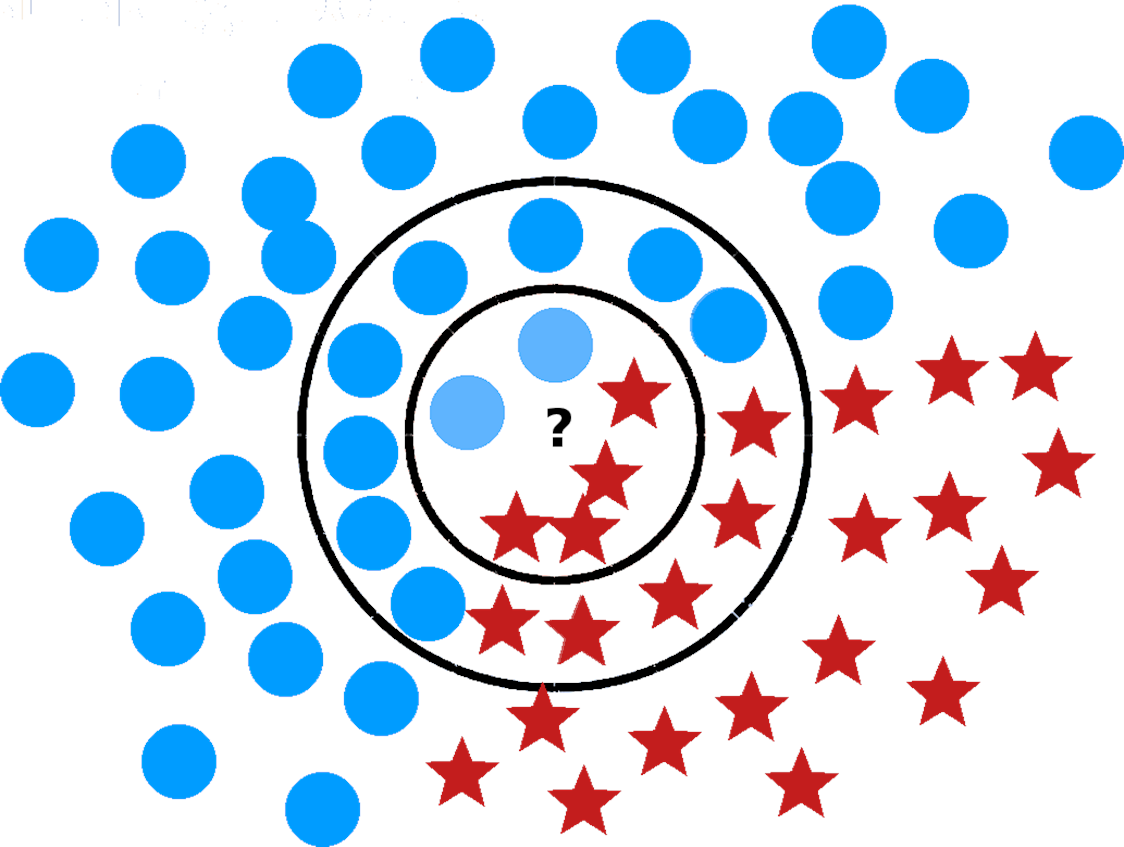
\includegraphics[height=0.85\textheight]{Images/kNN} \\ $k$ nearest neighbours
\end{center}
\newpage\ \\ \begin{center}
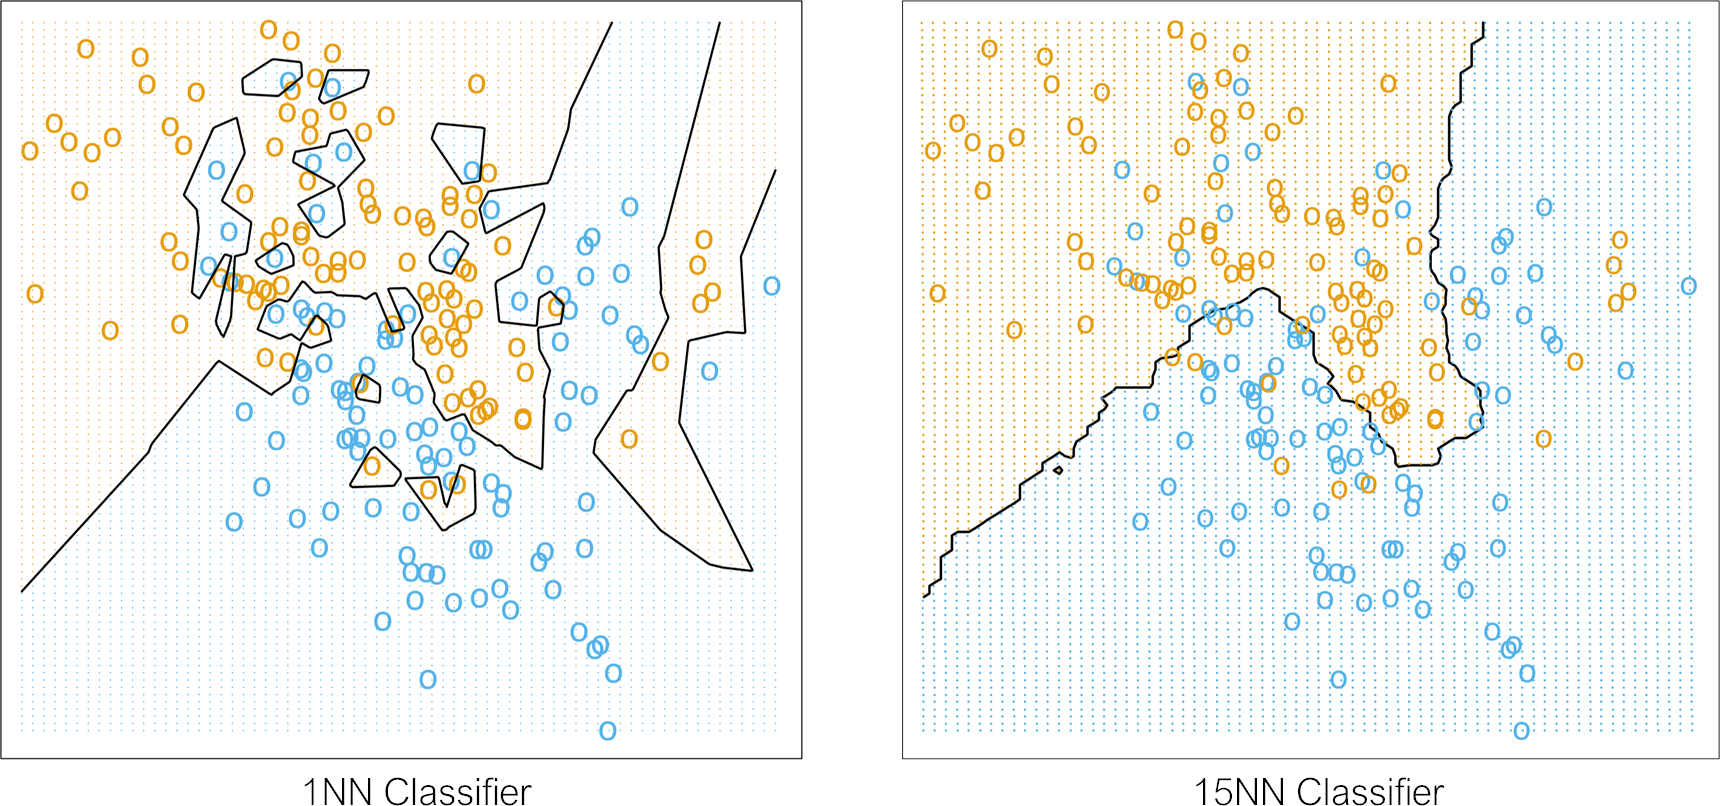
\includegraphics[width=\textwidth]{Images/kNNs} \newline [Tibshirani, Hastie, Friedman]
\end{center}
\newpage\ \\ \begin{center}
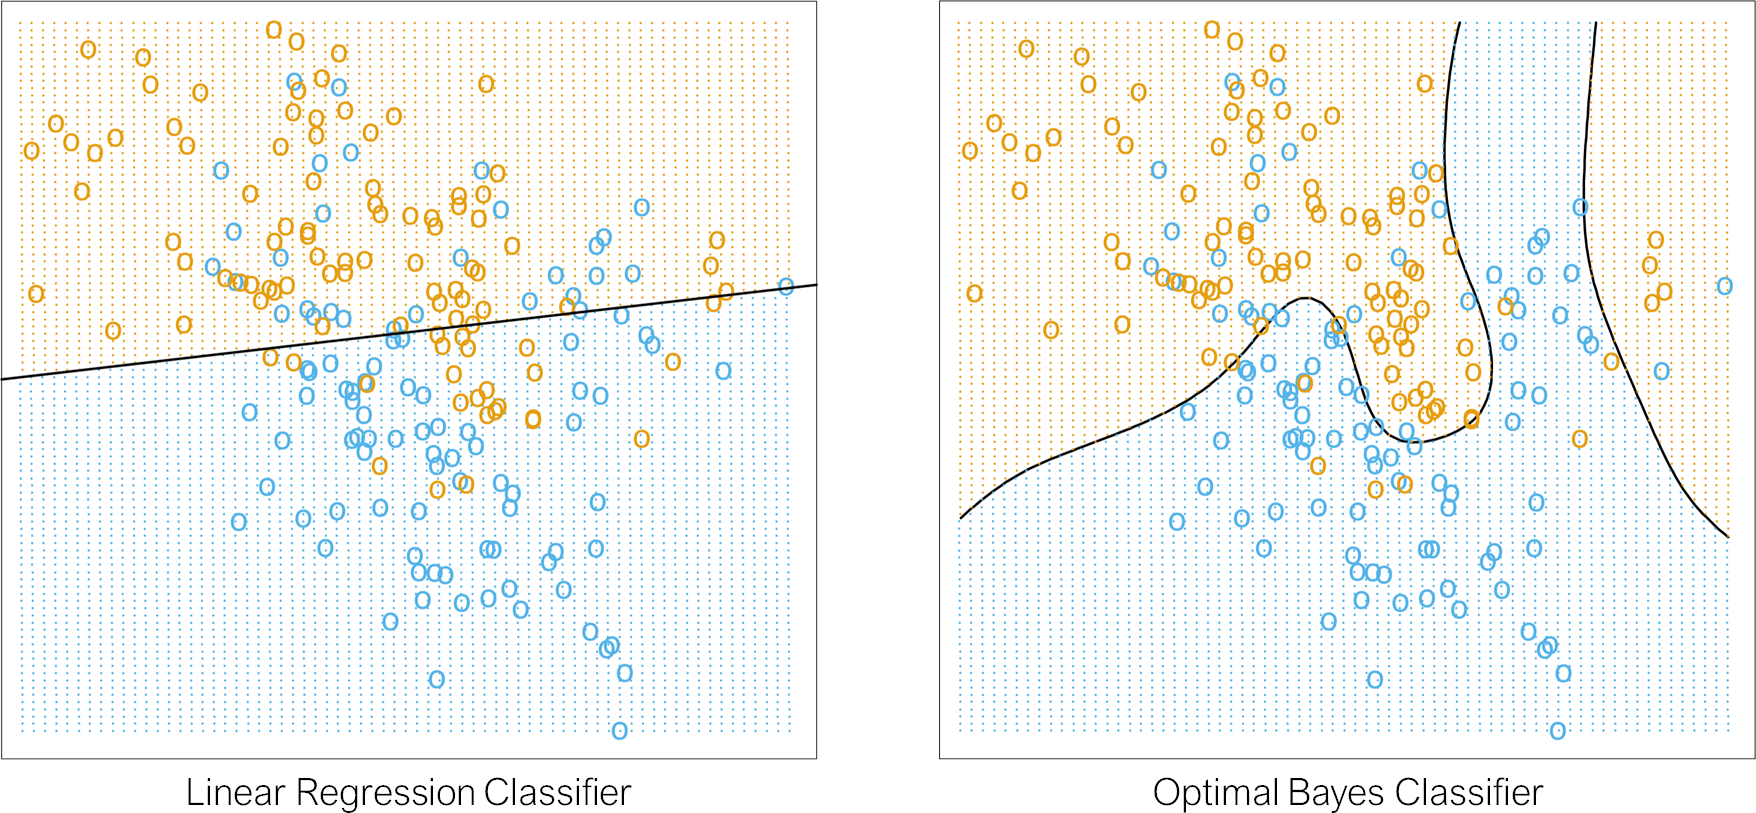
\includegraphics[width=\textwidth]{Images/RegBayes} \newline [Tibshirani, Hastie, Friedman]
\end{center}
\newpage\ \\ \begin{center}
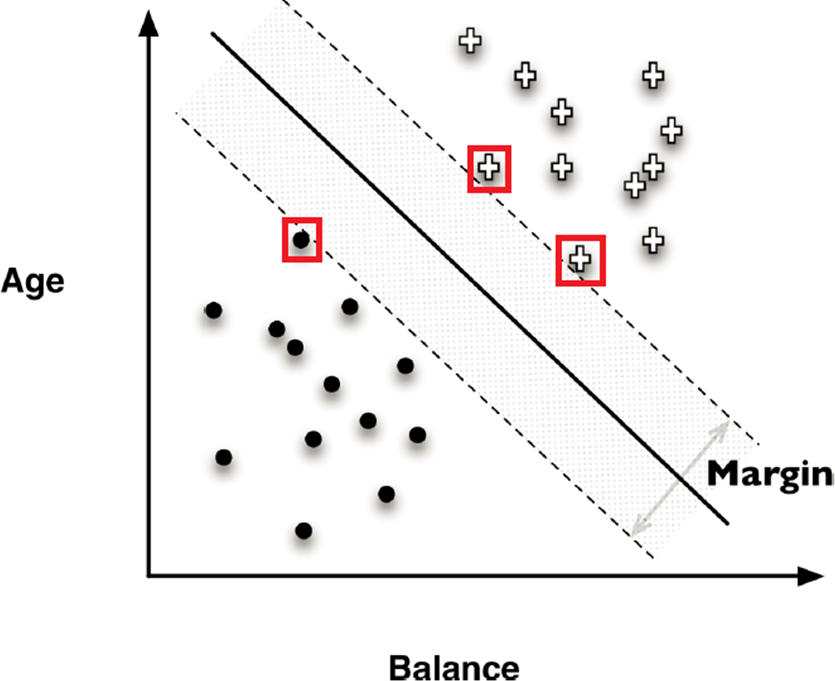
\includegraphics[height=0.5\textheight]{Images/SVM} \qquad 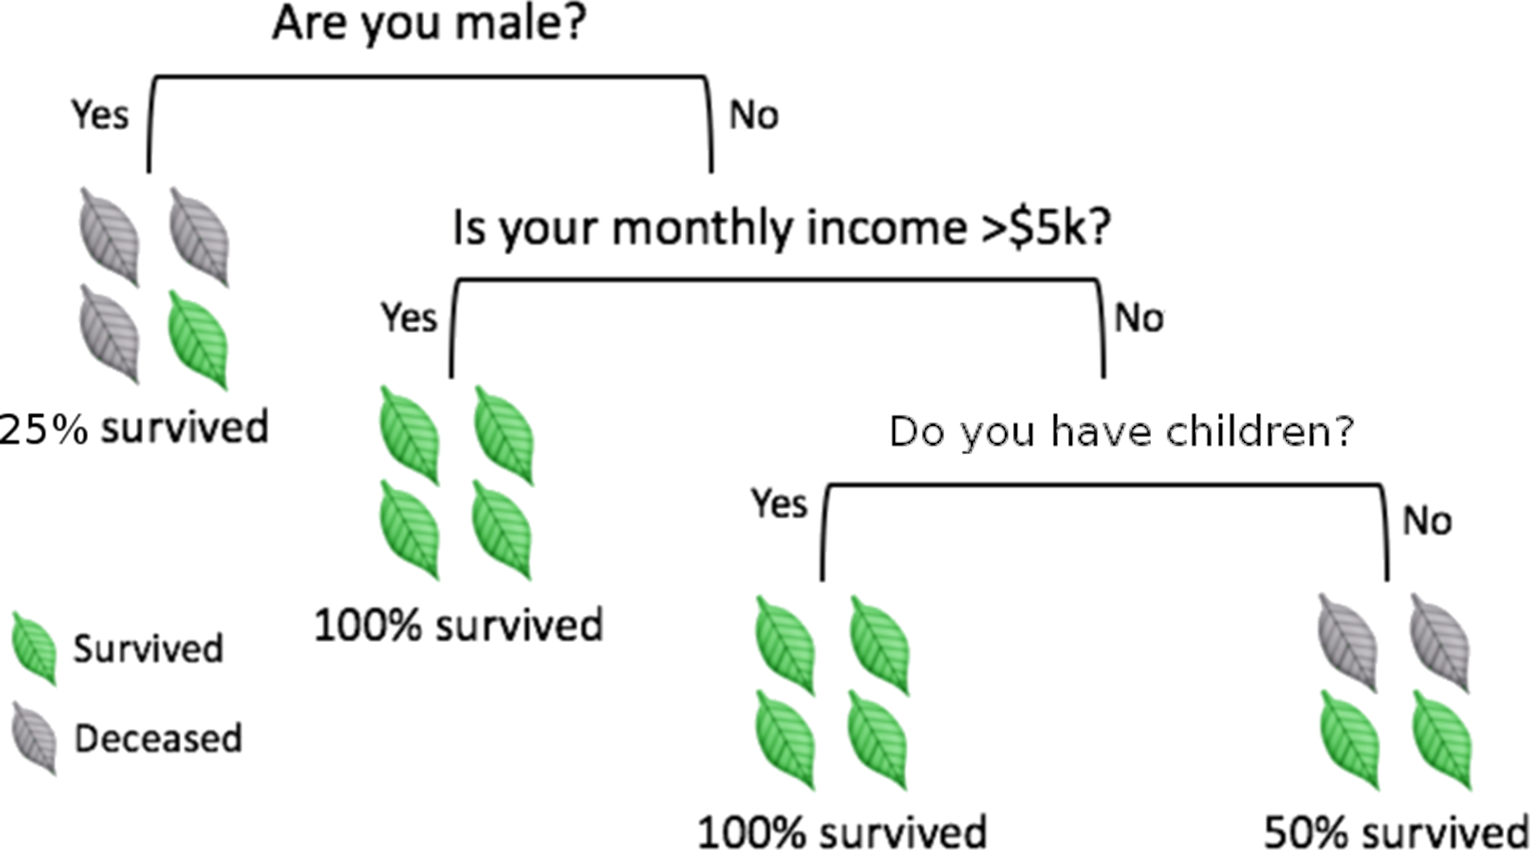
\includegraphics[height=0.5\textheight]{Images/DecisionTree} \newline Support vector machines (left), decision tree (right) \newline  [Foster and Provost, Ng and Soo]
\end{center}


\newpage \ \\ \noindent Another SL approach: estimate the \textbf{relative abnormality} of observations. 
\newl 
Estimating the probability that an observation $\mathbf{x}_1$ is anomalous $\Longrightarrow$ difficult; \\ 
Determining it is more likely to be anomalous than another $\mathbf{x}_2$ $\Longrightarrow$ easier. (We write $\mathbf{x}_1\succeq \mathbf{x}_2$.) \newl Let $k_i\in\{1,\ldots,m\}$ be the rank of the $i^{\text{th}}$ \textbf{true outlier}, $i\in \{1,\ldots,n\}$, in the sorted list of suspicious observations $$\mathbf{x}_1\succeq \mathbf{x}_{k_1}\succeq \cdots\succeq\mathbf{x}_{k_i}\succeq \cdots \mathbf{x}_{k_n}\succeq \mathbf{x}_m,\quad n\leq m;$$ the \textbf{rank power} of the algorithm is $$\text{RP}=\frac{n(n+1)}{2\sum_{i=1}^nk_i}.$$ \newpage\ \\ \noindent When the $n$ actual anomalies are ranked in (or near) the top $n$ suspicious observations, we have $$\sum_{i=1}^nk_i\approx \sum_{i=1}^ni =\frac{n(n+1)}{2} \Longrightarrow \text{RP}\approx 1.$$ As with most performance evaluation metrics, a single raw number is meaningless -- it needs to be compared to other algorithms. \newl Other SL performance evaluation metrics include: 
\begin{itemize}
\item \textbf{AUC} --  the probability of ranking a randomly chosen anomaly higher than a randomly chosen normal observation (higher is better);
\item \textbf{probabilistic AUC} -- a calibrated version of AUC. 
\end{itemize}
\newpage \ \\ \noindent 
The \textbf{rare occurrence} problem can be tackled by using: 
\begin{itemize}
\item a \textbf{manipulated training set} (oversampling, undersampling, generating artificial instances); 
\item \textbf{specific SL AD algorithms} (CREDOS, PN, SHRINK);
\item \textbf{boosting algorithms} (SMOTEBoost, RareBoost);
\item \textbf{cost-sensitive classifiers} (MetaCost, AdaCost, CSB, SSTBoost), 
\item etc. 
\end{itemize}
See A.Lazarević {et al.} [2004], \textit{Data Mining for Analysis of Rare Events: A Case Study in Security, Financial and Medical Applications} for more information.
\newpage\ \\ \noindent 
The rare (anomalous) class can be \textbf{oversampled} by duplicating the rare events until the data set is \textbf{balanced} (roughly the same number of anomalies and normal observations). \newl This does not increase the overall level of information, but it will increase the  mis-classification cost.\newl 
They majority class (normal observations) can also be \textbf{undersampled} by randomly removing: 
\begin{itemize}
\item ``near miss'' observations or
\item or observations far from anomalous observations.
\end{itemize}
Some loss of information has to be expected (and overly general rules).
\newpage \
\begin{center}
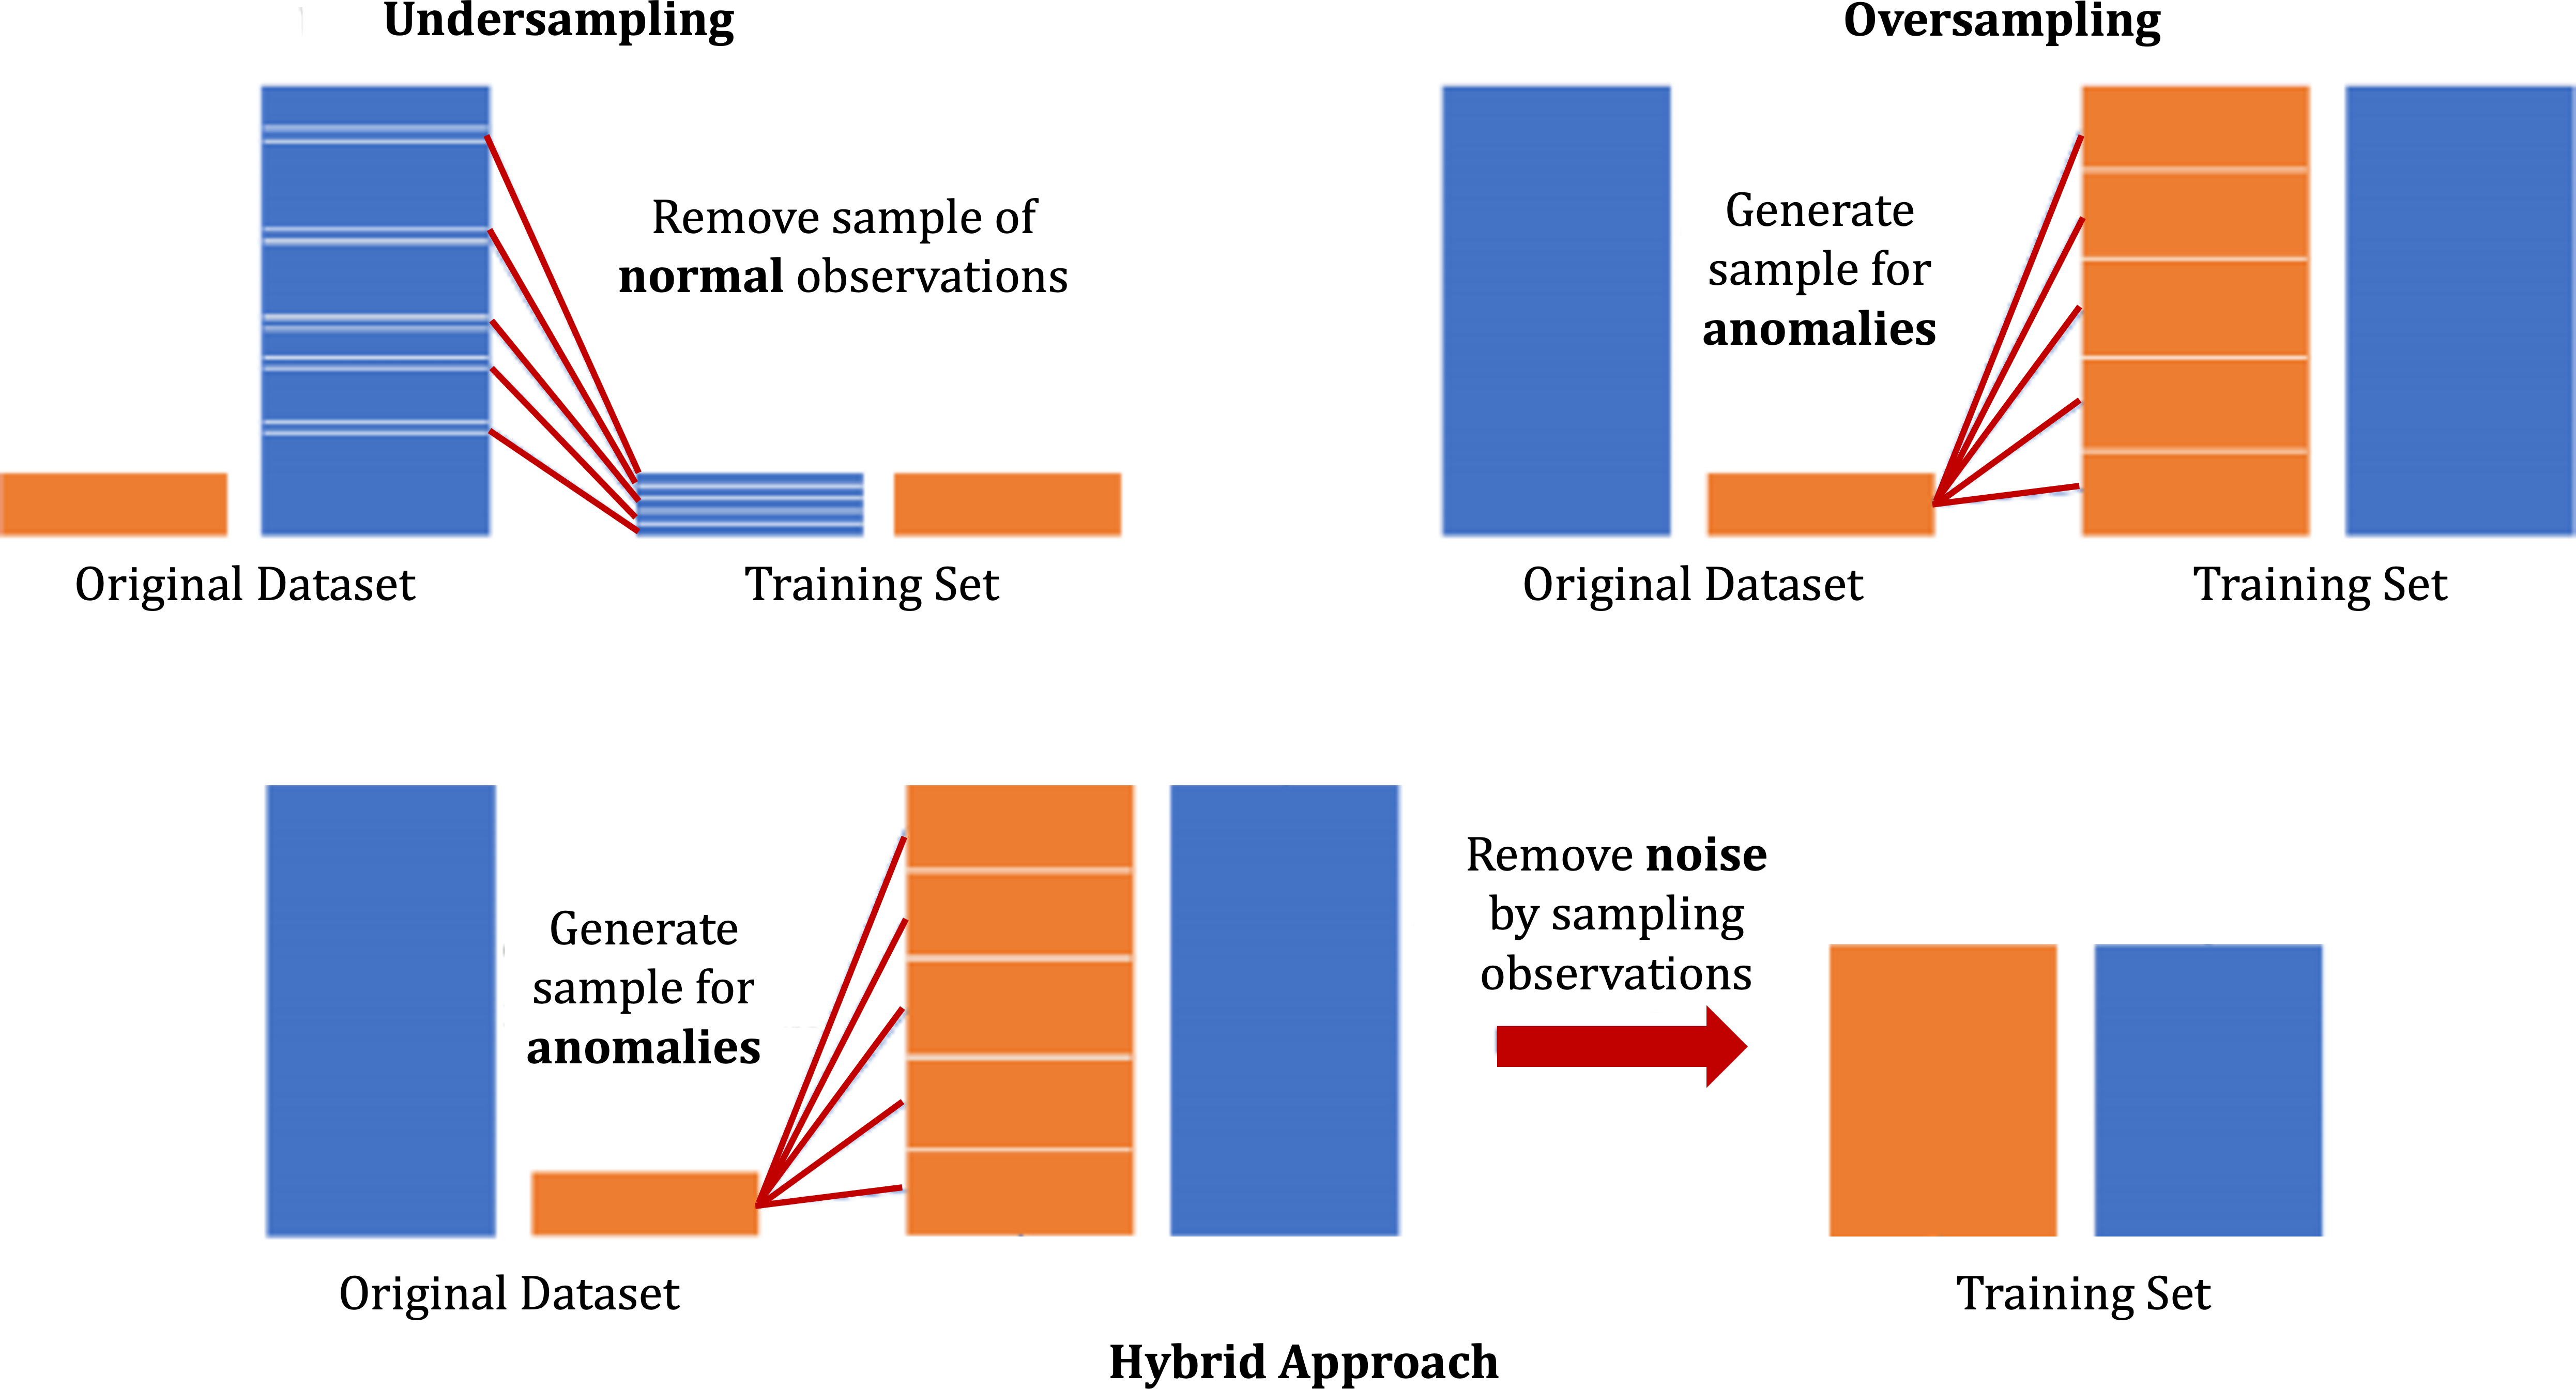
\includegraphics[height=0.8\textheight]{Images/OUHS.png} \newline [Le et al., A Hybrid Approach Using Oversampling Technique and Cost-Sensitive Learning for Bankruptcy Prediction]
\end{center}
\newpage\ 
\begin{center}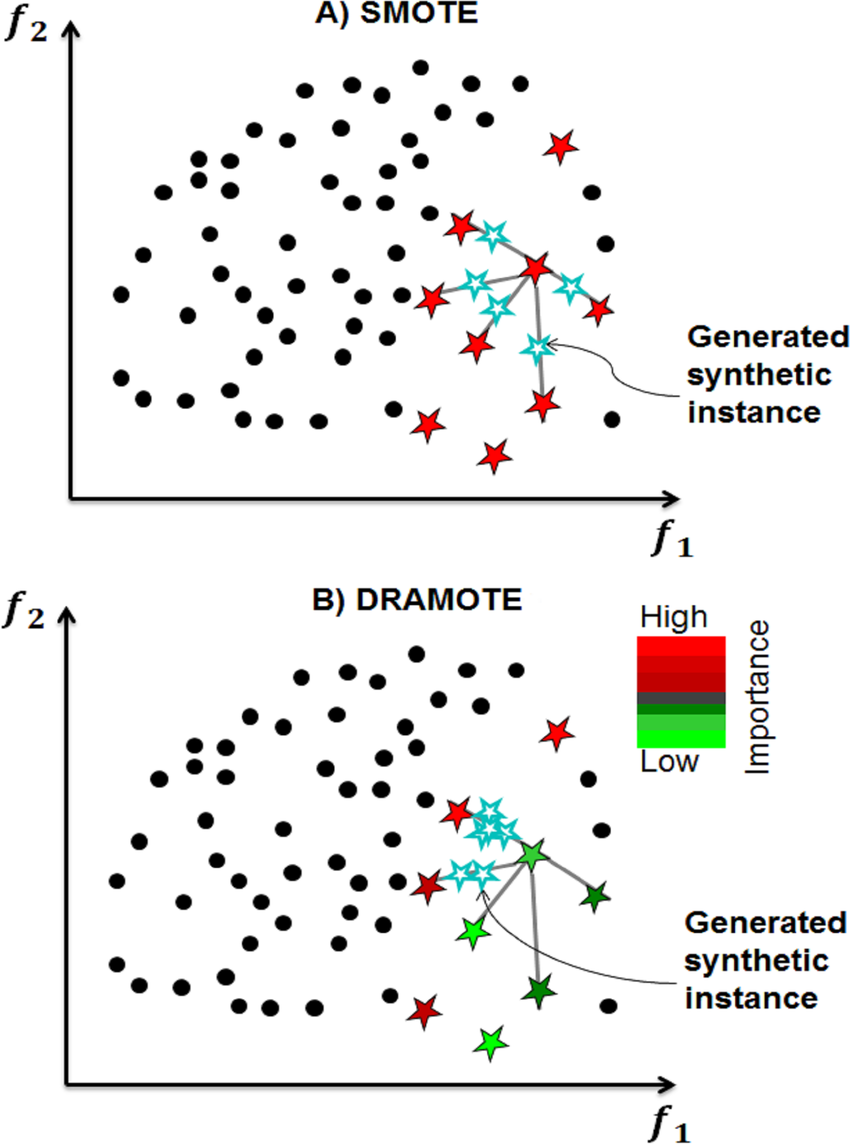
\includegraphics[height=0.85\textheight]{Images/SMOTE.png} \\ Generating artificial cases with SMOTE and DRAMOTE [Soufan, et al.] 
\end{center}\newpage
\begin{center}
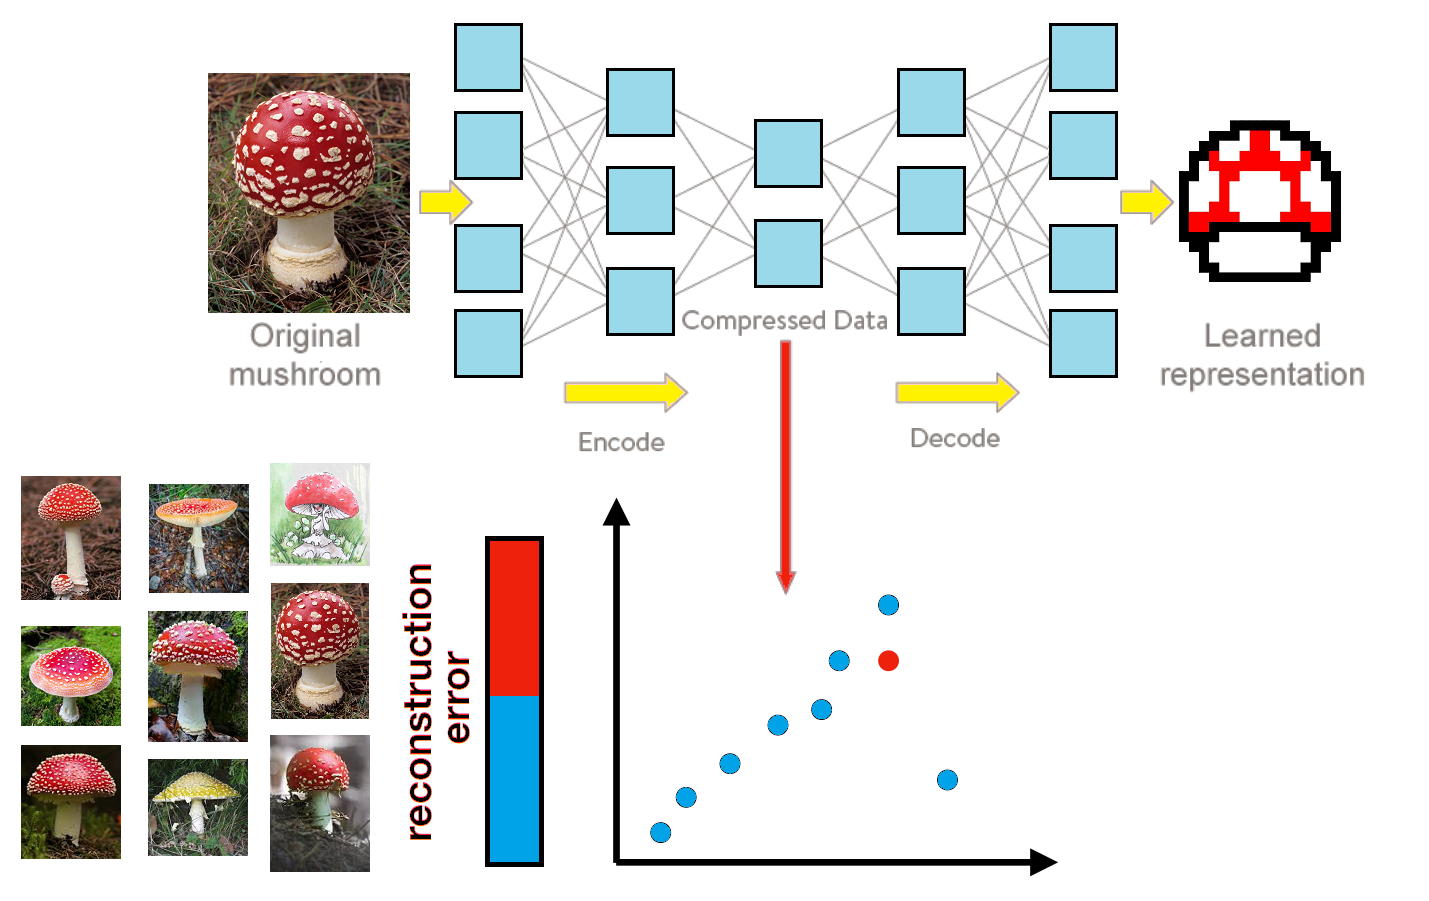
\includegraphics[width=\textwidth]{Images/autoencoder2.png}
\end{center}
\newpage \ \\ \noindent
\noindent \textbf{Autoencoders} learn a compressed representation of the data (dimension reduction).
\newl The \textbf{reconstruction error} measures (in a sense) how much information is lost in the compression. 
\newl Anomaly detection algorithms can be applied to the compressed data:
\begin{itemize}
\item look for anomalous patters, and/or
\item anomalous reconstruction errors. 
\end{itemize}
[Previous slide adapted from Baron].
\newpage \ \\ \noindent On the \textbf{unsupervised} front,  anomalous/normal labels are not used:
\begin{itemize}
\item anomalies are those observations that are dissimilar to other observations;
\item \textbf{clusters} are groupings of similar observations, so 
\item observations without a natural cluster fit are potential anomalies. 
\end{itemize}
\textbf{Challenges:} 
\begin{itemize}
\item most clustering algorithms do not recognize potential outliers (DBSCAN and variants are exceptions), and 
\item finding an appropriate measure of similarity/dissimilarity of observations is difficult (different measures often lead to different cluster assignments).  \end{itemize}
\newpage\  
\begin{center}
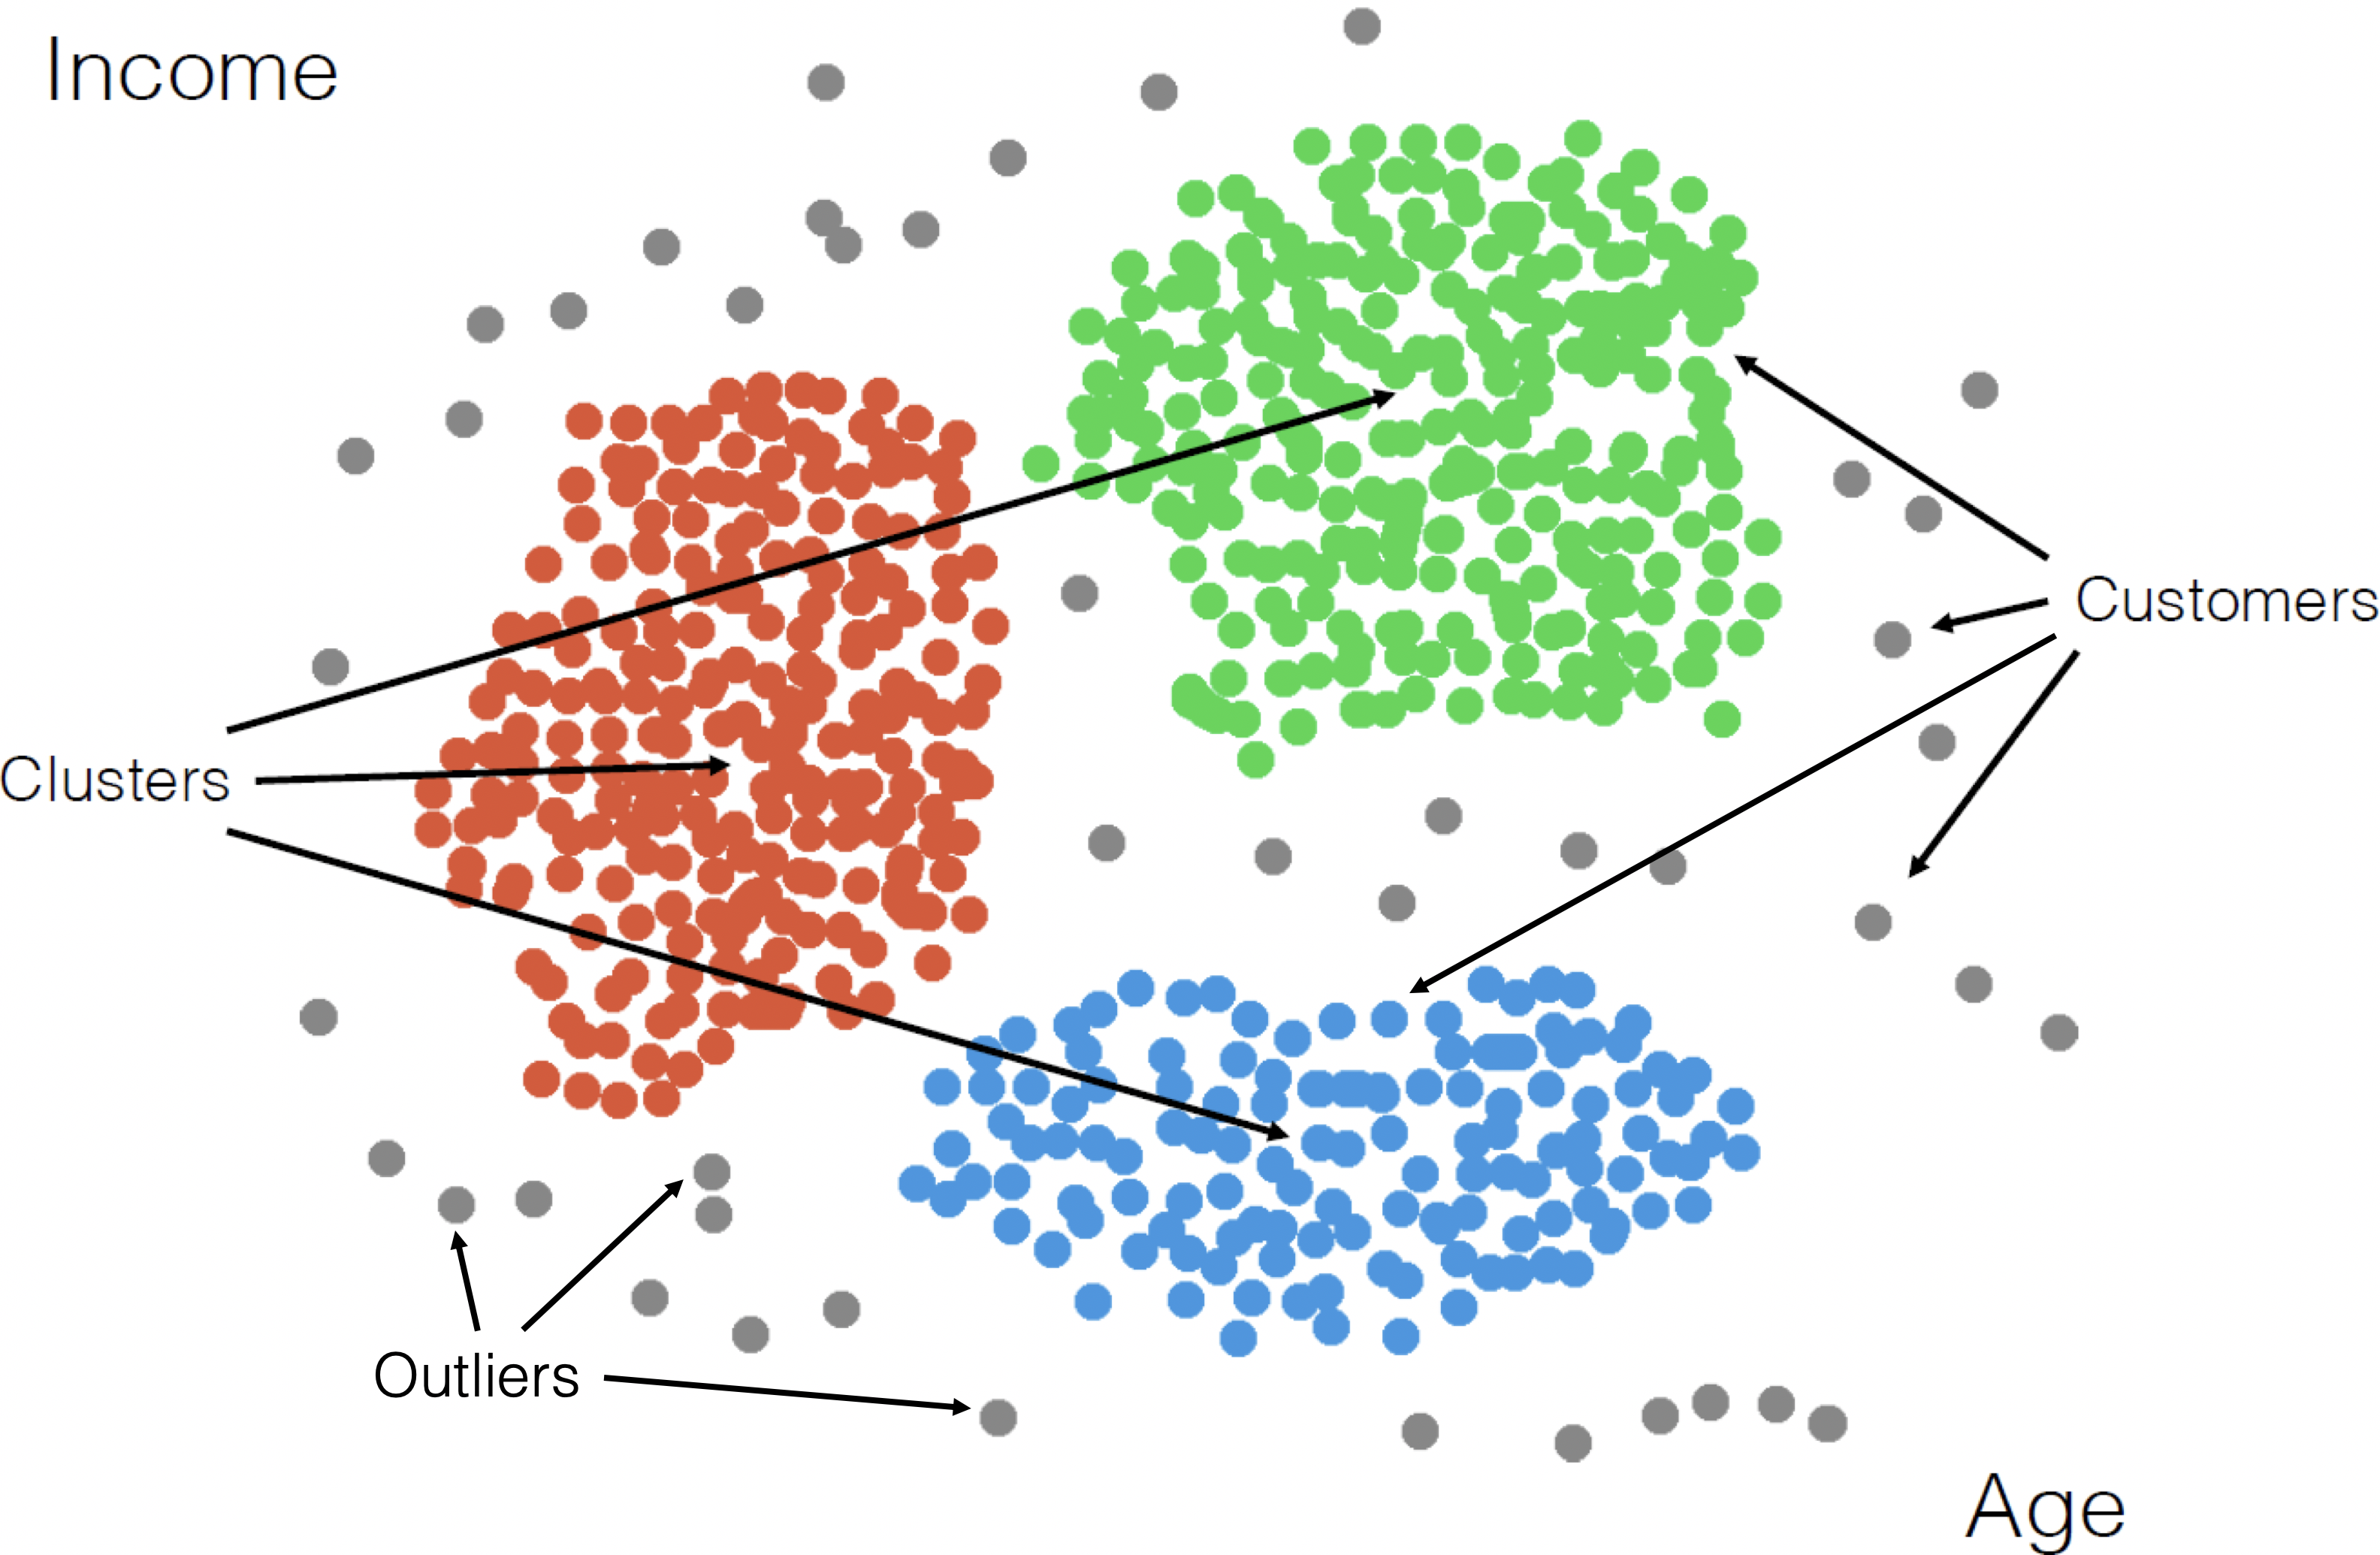
\includegraphics[width=0.75\textwidth]{Images/clustering2_EN.png} \\ 
Clusters of regular customers (red, green, blue) and potential anomalies/outliers (grey) in an artificial dataset.
\end{center}



\fh{\textcolor{darkestgreen}{6.2 -- Quantitative Methods of Anomaly Detection}} \label{6.2} 

\noindent Cluster-based methods are not the only types of UL anomaly detection methods.
\begin{itemize}
\item \textbf{Distance-based methods:} distance to all points, distance to $k$ nearest neighbours ($k$NN),  average distance to $k$NN, median distance to $k$NN, etc.
\item \textbf{Density-based methods:} local outlier factor (LOF), isolation forest, HDBSCAN, etc.
\end{itemize}

\fh{6.2.1 -- Distance-Based Methods} \label{6.2.1}
\noindent We find anomalous observations by  comparing them to other observations (\textbf{anomalies are relative, not absolute}). \newl In the \textbf{distance-based context}, the natural way to compare observations is  to consider their \textbf{distance from a subset of observations}: increasing distance being increasingly \textbf{suggestive} of anomalous status.
\newl \textbf{Requirement:} a \textbf{distance function} or a \textbf{pre-computed table of pair-wise distances} (in discrete case). 
\newl The choice of subsets and distance functions  distinguish the different distance-based algorithms.
\fh{Notation} \begin{itemize}
\item $D \subset \mathbb{R}^n$ is an $n$-dimensional (numerical) data set
\item $\mathbf{p},\mathbf{q}\in D$ are specific observations in $D$
\item $P \subset D$ is a subset of $D$
\item $d: D \times D \to \mathbb{R}$ is a distance function on $D\subset \mathbb{R}^n$
\item the distance between $\mathbf{p}$ and $\mathbf{q}$ is written $d(\mathbf{p},\mathbf{q})$
\newpage\ \item the output of an anomaly detection algorithm is a function $a : D \to \mathbb{R}$
\item $a(\mathbf{p})$ is a number that describes how anomalous $\mathbf{p}$ is \item 
if $a(\mathbf{p}) < a(\mathbf{q})$ for $\mathbf{p},\mathbf{q} \in D$, then $\mathbf{p}$ is \textbf{less anomalous} than $\mathbf{q}$
\item $\alpha \in \mathbb{R}$ is the \textbf{absolute anomaly threshold}
\item  any $\mathbf{p} \in D$ for which $a(\mathbf{p}) > \alpha$ is \textbf{absolutely anomalous}
\end{itemize}
\fh{Similarity Measures}
\noindent A \textbf{similarity measure} is a real-valued function that describes the \textbf{similarity between two objects}.
\newl A common construction for the similarity $w$ between two points $\mathbf{p},\mathbf{q}$: $$w(\mathbf{p},\mathbf{q})=\frac{1}{1+d(\mathbf{p},\mathbf{q})}, \quad \text{for some distance }d.$$ \textbf{Note:}  $w\to 1$ as $d\to 0$, and $w\to 0$ as $d\to \infty$. \newl  
Similarity measures can also be constructed between \textbf{probability distributions} (see Hellinger distance). \newpage\  \begin{center}
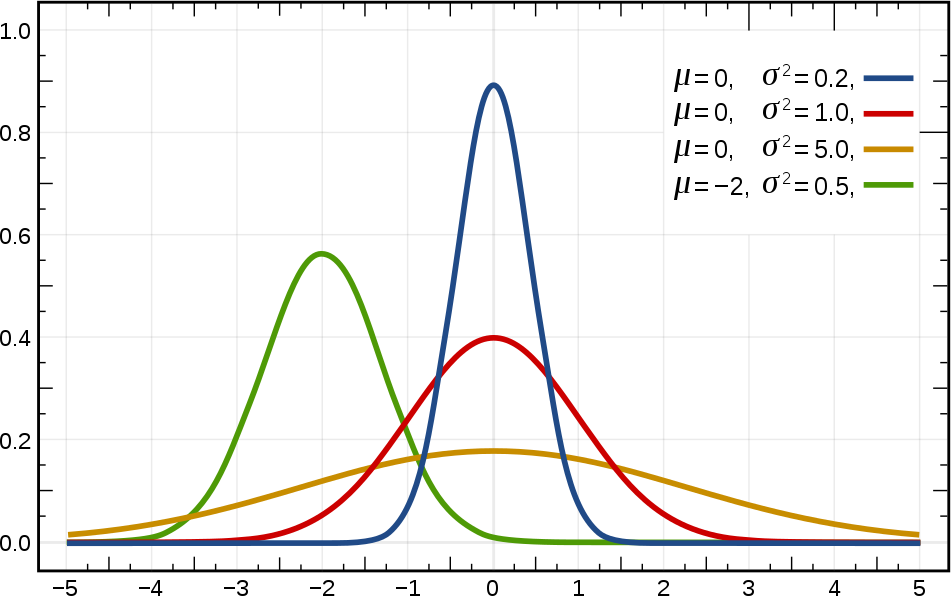
\includegraphics[width=0.8\textwidth]{Images/distributions.png}
\end{center}\newpage \ \\ \noindent
We can think of a single point $\mathbf{p}$ as a probability distribution (with $0\%$ chance of drawing another point). \newl The distance between that point and any other distribution with mean $\mathbf{\mu}$ and covariance matrix $\mathbf{\Sigma}$ can be given using the \textbf{Mahalanobis framework}:

$$
M(\mathbf{p})=\sqrt{(\mathbf{p} - \mathbf{\mu})^{\!\top} \mathbf{\Sigma}^{-1} (\mathbf{p} - \mathbf{\mu})} \quad \text{(BACON).}
$$

\noindent Alternatively, if $\mathbf{p}$ and $\mathbf{q}$ are drawn from the same distribution with covariance $\Sigma$, then the Mahalanobis distance is a dissimilarity measure between $\mathbf{p}$ and $\mathbf{q}$: 

$$
d_M(\mathbf{p},\mathbf{q})=\sqrt{(\mathbf{p} - \mathbf{q})^{\!\top} \mathbf{\Sigma}^{-1} (\mathbf{p} - \mathbf{q}).}
$$
\newpage\ \\ \noindent 
\textbf{Example:} consider a 4D-dataset drawn from a multivariate  $\mathcal{N}(\mathbf{\mu},\mathbf{\Sigma})$ with  
\small $$\mathbf{\mu}=(1,-2,0,1),\quad \mathbf{\Sigma}=\begin{pmatrix}1 & 0.5 & 0.7 & 0.5 \\ 0.5 & 1 & 0.95 & 0.3 \\ 0.7 & 0.95 & 1 & 0.3 \\ 0.5 & 0.3 & 0.3 & 1\end{pmatrix}.$$\normalsize
$100$ observations $\mathbf{p}_1$ to $\mathbf{p}_{100}$ are ``normal'': 
\small \begin{center}
\begin{tabular}{crrrr}
\textbf{stat} & $x_1\ \ $ & $x_2\ \ $ & $x_3\ \ $ & $x_4\ \ $ \\ \hline          
 min   & $-1.9049$  & $-4.4113$ & $-2.5324$ & $-1.9949$ \\ 
 $Q_1$ &  $ 0.3812$  & $-2.6464$ & $-0.6190$ & $ 0.3361$ \\ 
 med   &  $ 0.9273$  & $-2.0220$ & $-0.0506$ & $ 0.9381$ \\ 
 avg  &  $ 0.9374$  & $-1.9788$ & $ 0.0071$ & $ 0.9438$ \\ 
 $Q_3$ &  $ 1.4615$  & $-1.4002$ & $ 0.6296$ & $ 1.5906$ \\ 
 max   &  $ 3.4414$  & $0.5223$  & $ 2.0265$ & $ 2.8073$ \\
 \end{tabular}
\end{center}\normalsize
$2$ observations are ``anomalous'':  $\mathbf{z}_1=(1,1,1,1)$, $\mathbf{z}_4=(4,4,4,4)$. 
\newpage\ \begin{center}
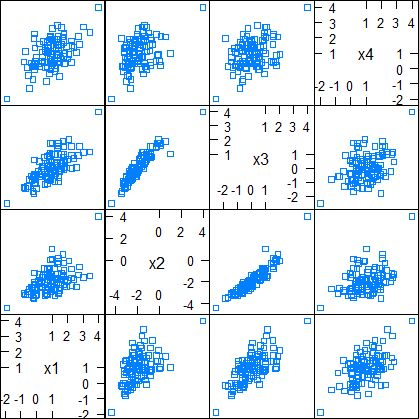
\includegraphics[height=0.8\textheight]{Images/Artificial_4D_Dataset} \\ Visually, it seems there might be $3$ outliers. 
\end{center} \newpage\ \begin{center}
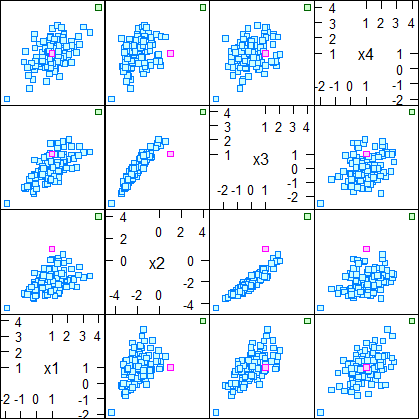
\includegraphics[height=0.92\textheight]{Images/Artificial_4D_Dataset_Groups}
\end{center}\newpage\ \\ \noindent In general, the mean vector and the covariance structure must be estimated from the data: 
\small $$\mathbf{\hat{\mu}}=(0.968, -1.891,0.056,0.974),\quad \mathbf{\hat{\Sigma}}=\begin{pmatrix}
0.900 & 0.569 & 0.665 &  0.503 \\
0.569 & 1.312 & 1.069 &  0.469 \\
0.665 & 1.069 & 0.992 &  0.397 \\
0.503 & 0.469 & 0.397 &  0.904 \end{pmatrix}.$$\normalsize
These are distinct from $\mathbf{\mu}$ and $\mathbf{\Sigma}$, but close enough to be explained by 
\begin{itemize}
\item sampling variation
\item $\mathbf{z}_1,\mathbf{z}_4\not\sim \mathcal{N}(\mathbf{\mu},\mathbf{\Sigma})$
\end{itemize}
To identify anomalous observations, compute the Mahalanobis distance from all points to the empirical distribution, and between all pairs.  
\newpage\ \begin{center}
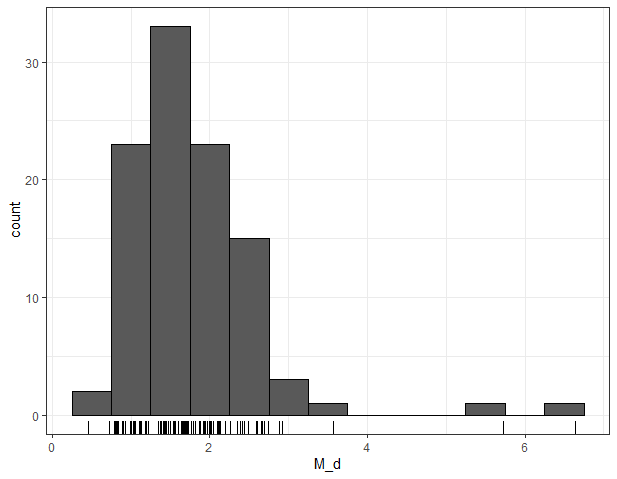
\includegraphics[height=0.8\textheight]{Images/Histogram_Md} \\ Histogram of Mahalanobis distances to empirical distribution.
\end{center}
\newpage\ \begin{center}
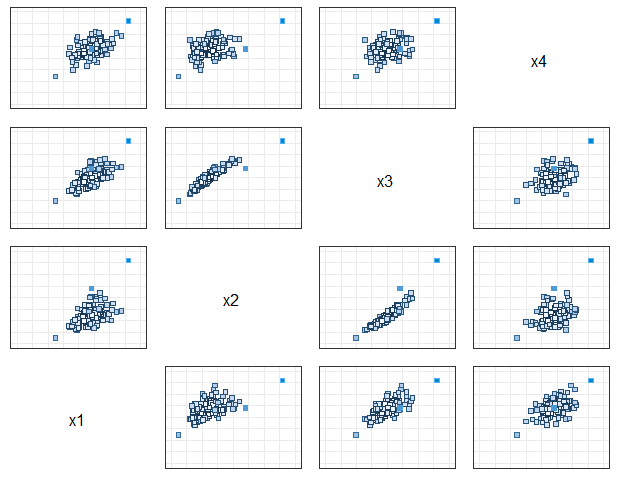
\includegraphics[height=0.85\textheight]{Images/Artificial_4D_Dataset_Md_scores} \\ Scatter plot of Mahalanobis distances to empirical distribution.
\end{center}\newpage\ \\  \begin{center}
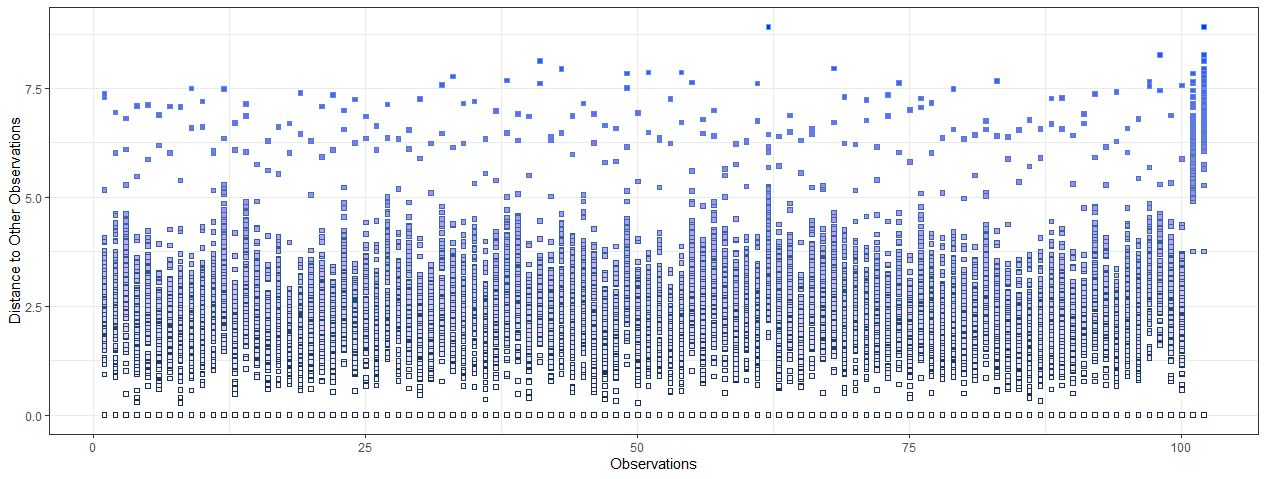
\includegraphics[width=\textwidth]{Images/Artificial_4D_Datasets_Pairs} \\ Mahalanobis distances between each pair (empirical distribution). \\ Notice observations $101$ and $102$, as well as the diffuse cloud of points above the value $5.0$.
\end{center}\newpage\ \\  \begin{center}
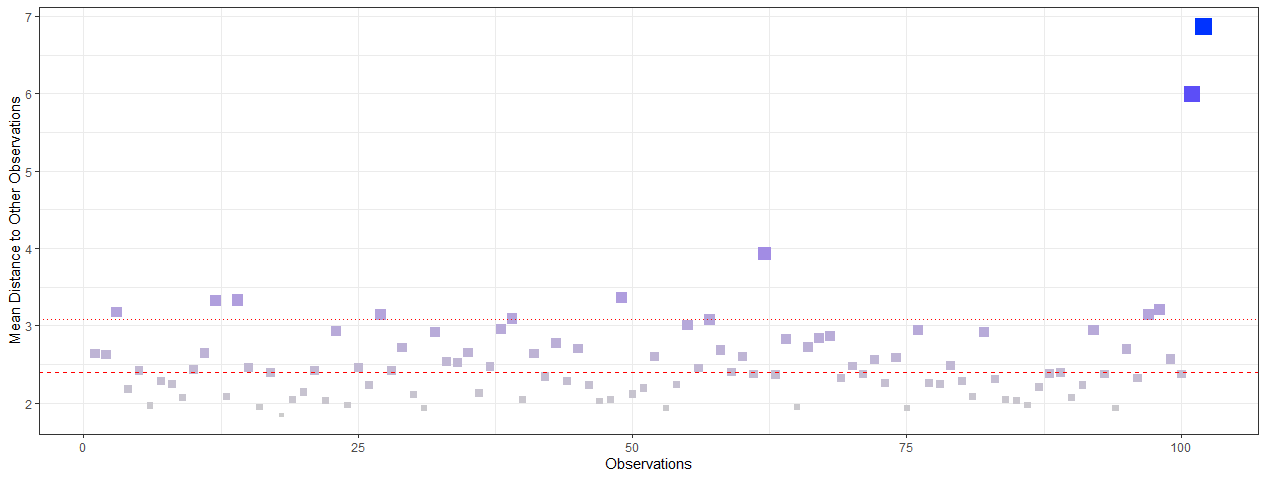
\includegraphics[width=\textwidth]{Images/Artificial_4D_Dataset_MeanDist} \\ Mean Mahalanobis distances between each pair (empirical distribution). \\ Notice observations $101$ and $102$ again. The red lines represent the median mean distance, and $1$ standard deviation the median mean distance. \\ The Mahalanobis framework seems to identify $2$ outliers. 
\end{center}\newpage\ \\ \noindent If  $\Sigma$ is diagonal, then 

$$
d_M(\mathbf{p},\mathbf{q})=\sqrt{\sum_{i=1}^n \frac{(p_i - q_i)^2}{\sigma_i^2}},
$$
where $\sigma_i^2$ is the variance along the $i$-th dimension.
\newl If $\Sigma$ is the identity matrix, then we recover the \textbf{Euclidean distance}

$$
d_2(\mathbf{p},\mathbf{q})=\sqrt{\sum_{i=1}^n (p_i - q_i)^2}.
$$
\noindent In an anomaly detection context, a \textbf{linear normalization} is usually applied to each dimension so that each entry lies in the hypercube  $[-1,1]^n$.
\newpage\ \\ \noindent The \textbf{Minkowski distance} of order $p$ is a generalization of the Euclidean distance:
$$
d_p(\mathbf{p},\mathbf{q})=\left( \sum_{i=1}^n |p_i - q_i|^p \right)^{1/p}.
$$
\begin{itemize}
\item For $p=1$, we recover the \textbf{Manhattan distance}: $$d_1(\mathbf{p},\mathbf{q})=\sum_{i=1}^n|p_i-q_i|;$$ 
\item for $p=\infty$, we recover the \textbf{supremum} (Chebychev) \textbf{distance} $$d_{\infty}(\mathbf{p},\mathbf{q})=\max_{i=1}^n \left\{|p_i - q_i|\right\}.$$ 
\end{itemize}
\newpage\ \\ \noindent The Minkowski distance $d_p$ is only an actual distance function (a \textbf{metric}) when  $p \geq 1$, but an exception is made for 
$$
d_{-\infty}(\mathbf{p},\mathbf{q})=\min_{i=1}^n \left\{|p_i - q_i|\right\}.
$$
When working with categorical data (such as in one-hot encoding of text), it can be useful to use distances for binary vectors.\newl  Let $\mathbf{p},\mathbf{q}\in  \{0,1\}^n$.\newl 
The \textbf{Hamming distance} between $\mathbf{p}$ and $\mathbf{q}$ counts the number of positions where they differ: 
$$d_H(\mathbf{p},\mathbf{q})=\sum_{i=1}^n|p_i-q_i|.$$
\newpage\ \\ \noindent The \textbf{Jaccard similarity} of two datasets $P$ and $Q$, is defined as the size of their intersection divided by the size of their union
$$
J(P,Q)
= \frac{|P \cap Q|}{|P \cup Q|}
= \frac{|P \cap Q|}{|P| + |Q| - |P \cap Q|}
$$
Their \textbf{Jaccard distance} is $d_J(P,Q)=1 - J(P,Q)$. This can be extended to binary vectors $\mathbf{p}$ and $\mathbf{q}$. \newl Consider an arbitrary set $D=\{x_1,x_2,\ldots,x_n\}$. We build $P$ as follows: if $p_i=1$ then $x_i\in P$; otherwise $x_i\not\in P$. Similarly for $Q$. \newl Then $|P|=\sum p_i$, $|Q|=\sum q_i$, $|P\cap Q|=\sum p_iq_i=\mathbf{p}\cdot\mathbf{q}$ and  
$$d_J(\mathbf{p},\mathbf{q})=d_J(P,Q)=1-J(P,Q)=1-\frac{\mathbf{p}\cdot \mathbf{q}}{\sum (p_i+q_i)-\mathbf{p}\cdot \mathbf{q}}.$$ 
\newline\newline
Finally, let $\mathbf{p},\mathbf{q}\neq \mathbf{0}$. Recall that 
$\mathbf{p} \cdot \mathbf{q} 
= \lVert p \rVert \lVert q \rVert \cos\theta,$
where $\theta$ is the angle between $\mathbf{p}$ and $\mathbf{q}$.\newl  The \textbf{cosine similarity} between $\mathbf{p}$ and $\mathbf{q}$ is 
$$
\cos\theta
= \frac{p \cdot q}{\lVert p \rVert \lVert q \rVert}
= \frac{\sum_{i=1}^n p_i q_i}{\sqrt{\sum_{i=1}^n p_i^2} \sqrt{\sum_{i=1}^n q_i^2}}.
$$
This also holds $\mathbf{p},\mathbf{q}$ are non-binary. The value ranges between $1$ and $-1$:
\begin{itemize}
\item $\cos \theta= 1$ when $\mathbf{p}=\mathbf{q}$;
\item $\cos \theta= -1$ when $\mathbf{p}=-\mathbf{q}$, and \item $\cos \theta =0$ when $\mathbf{p}$ and $\mathbf{q}$ are perpendicular.
\end{itemize}
\newpage
\begin{center}
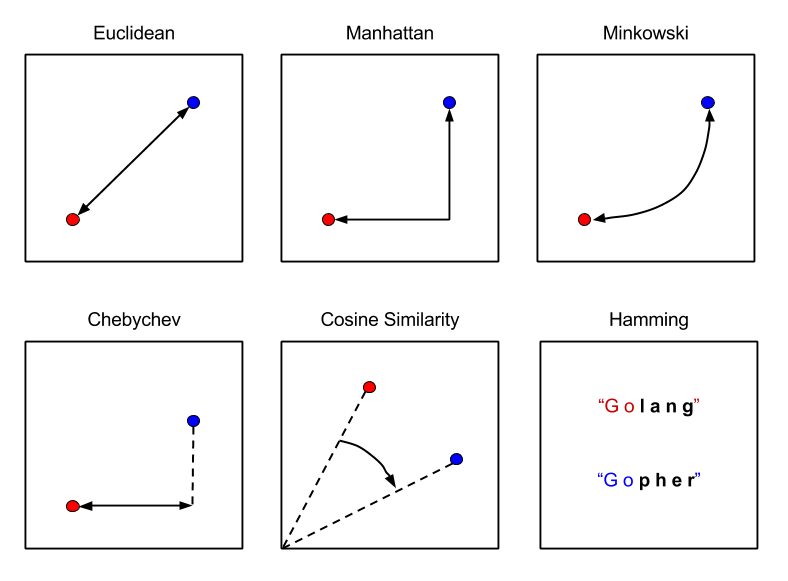
\includegraphics[width=0.9\textwidth]{Images/distances_comparison}
%Machine Learning with Go, Whitenack
\end{center}
\fh{Distance-Based Approaches}
\normalsize \noindent Finding the right distance function to use for anomaly detection is \textbf{NOT AN EASY TASK} -- contextual understanding and domain expertise are required.\newl  
Any such distance function can be used as the basis for anomaly detection algorithms (the ideas can also be extended to more complex algorithms).
\newline\newline Given some distance function $d$, dataset $D$, and integers $k,\nu\leq |D|$, 
the \textbf{distance to all points} (DTAP) anomaly detection algorithm considers each point $\mathbf{p}$ in $D$ and adds the distance from $\mathbf{p}$ to every other point in $D$:
$$
a(\mathbf{p}) 
= \sum_{\mathbf{q}\neq \mathbf{p} \in D} d(\mathbf{q}, \mathbf{p}).
$$
\newpage\ \\ \noindent The $\nu$ points with largest values for $a$ are then said to be \textbf{anomalous according to} $a$. \newl This approach often selects the most extreme observations as anomalous, which may be of limited use in practice. 
\newl The \textbf{distance to nearest neighbour} (DTNN) algorithm uses 
$$
a(\mathbf{p}) 
= \min_{\mathbf{q}\neq \mathbf{p} \in D} \{d(\mathbf{q}, \mathbf{p})\},
$$
with a similar definition for the $\nu$ anomalous points. 
\newl The \textbf{average distance to $k$ nearest neighbours} and \textbf{median distance to $k$ nearest neighbours} are defined similarly. 
\newpage
\begin{center}
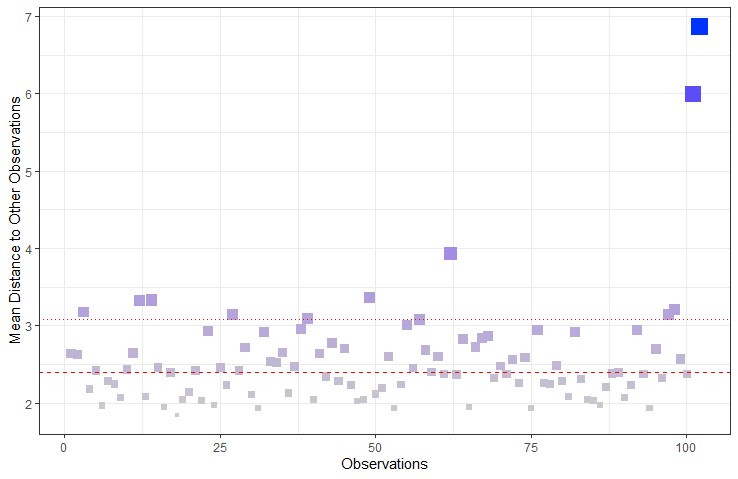
\includegraphics[width=\textwidth]{Images/AD_M}
\end{center}
\newpage
\begin{center}
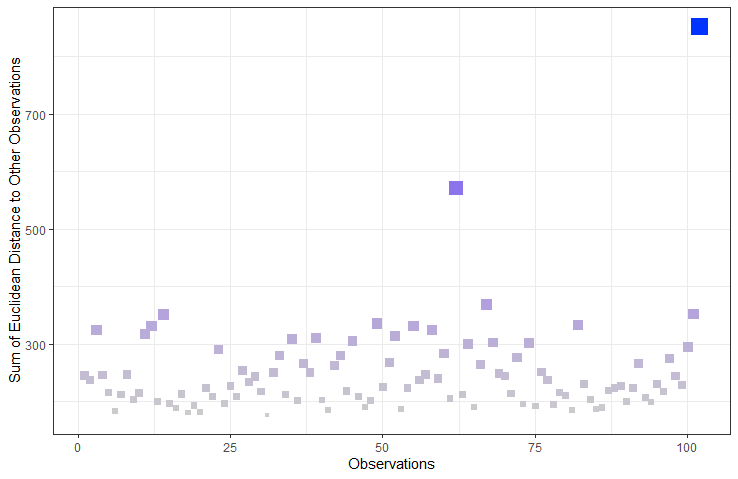
\includegraphics[width=\textwidth]{Images/AD_L2_sum}
\end{center}
\newpage
\begin{center}
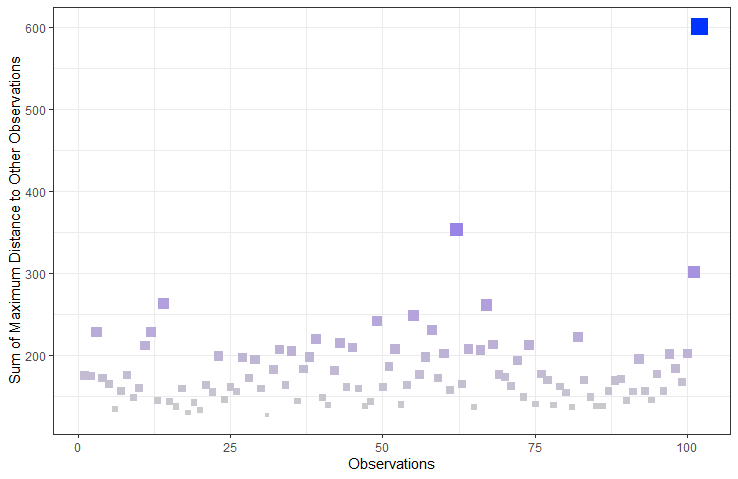
\includegraphics[width=\textwidth]{Images/AD_L0_sum}
\end{center}
\newpage
\begin{center}
\includegraphics[width=\textwidth]{Images/AD_L1_sum}
\end{center}
\newpage
\begin{center}
\includegraphics[width=\textwidth]{Images/AD_L1_2_sum}
\end{center}
\newpage
\begin{center}
\includegraphics[width=\textwidth]{Images/AD_L4_sum}
\end{center}
\newpage\ 
\begin{center}
\begin{tabular}{ccc}
\textbf{Mahalanobis} & 
\textbf{Euclidean}   & 
\textbf{Supremum}    \\ \hline
$102$ & $102$ & $102$ \\
$101$ & $62$  & $62$  \\
$67$  & $67$  & $101$ \\
$14$  & $101$ & $14$  \\
$12$  & $14$  & $67$  \\
& & \\
\textbf{Manhattan}   &
\textbf{Minkowski $(p=0.5)$} & \textbf{Minkowski $(p=4)$} \\ \hline
$102$ & $102$ & $102$ \\
$62$ & $62$  & $62$  \\
$67$  & $67$  & $101$ \\
$14$  & $14$ & $67$  \\
$49$  & $49$  & $14$  \\
& & \\
\end{tabular} \\ 
DTAP anomalies ($\nu=5$), for various distances; unscaled data.
\end{center}
\newpage\ \\  
\begin{center}
\begin{tabular}{ccc}
\textbf{Euclidean} & 
\textbf{Supremum}   & 
\textbf{Manhattan}    \\ \hline
$102$ & $102$ & $102$ \\
$61$ & $62$  & $62$  \\
$67$  & $14$  & $14$ \\
$101$  & $55$  & $67$  \\
$14$  & $49$  & $49$  \\
& & \\
\end{tabular} \\ 
DTAP anomalies ($\nu=5$), for various distances; scaled data.
\end{center}
The rankings change according to the selected distance function, the data scaling, and the choice of algorithm (see following slides). \newl How do we make these decisions, then?   
\newpage
\begin{center}
\includegraphics[width=\textwidth]{Images/AD_L2_min}
\end{center}
\newpage
\begin{center}
\includegraphics[width=\textwidth]{Images/AD_L0_min}
\end{center}
\newpage
\begin{center}
\includegraphics[width=\textwidth]{Images/AD_L1_min}
\end{center}
\newpage
\begin{center}
\includegraphics[width=\textwidth]{Images/AD_L1_2_min}
\end{center}
\newpage
\begin{center}
\includegraphics[width=\textwidth]{Images/AD_L4_min}
\end{center}
\newpage\ 
\begin{center}
\begin{tabular}{ccc}
\textbf{Mahalanobis} & 
\textbf{Euclidean}   & 
\textbf{Supremum}    \\ \hline
$102$ & $102$ & $102$ \\
$101$ & $62$  & $62$  \\
$67$  & $101$  & $101$ \\
$14$  & $11$ & $12$  \\
$12$  & $12$  & $23$  \\
& & \\
\textbf{Manhattan}   &
\textbf{Minkowski $(p=0.5)$} & \textbf{Minkowski $(p=4)$} \\ \hline
$102$ & $102$ & $102$ \\
$62$ & $62$  & $62$  \\
$101$  & $101$  & $101$ \\
$12$  & $11$ & $12$  \\
$11$  & $23$  & $11$  \\
& & \\
\end{tabular} \\ 
DTNN anomalies ($\nu=5$), for various distances; unscaled data.
\end{center}


\fh{6.2.2 -- Density-Based Methods} \label{6.2.2} 
\noindent The flexibility in the choice of distance functions, scaling, and distance-based anomaly detection algorithm gives rise to different \textbf{anomaly rankings}. This is par for the course in the anomaly detection context. \newl Density-based approaches view points as anomalous if they occur in \textbf{low density regions}. Methods include: \begin{itemize}
\item \textbf{local outlier factors};
\item \textbf{DBSCAN}, and  
\item \textbf{isolation forests}.
\end{itemize}

\newpage
\begin{center}
\includegraphics[width=0.8\textwidth]{Images/IsoForest2.png} \newline Low-density areas as outlier nurseries [Baron].
\end{center}


\fh{Local Outlier Factor} % p110
\noindent The \textbf{Local Outlier Factor} (LOF) algorithm works by measuring the \textbf{local deviation} of each observation \textbf{from its $k$ nearest neighbours}.\newl An observation is said to be anomalous if the \textbf{deviation is large}.
\newl A \textbf{local $k-$region} around a point $\mathbf{p}$ is simply the set $N_k(\mathbf{p})$ of the $k$ nearest neighbours of $\mathbf{p}$ $\Longrightarrow$ need to select a distance measure. \newl 
Local $k-$regions have different extent from one observation to the next $\Longrightarrow$ each $\mathbf{p}$ has a \textbf{local density}. 
\newl Observations with anomalously small local density compared to its $k-$neighbours are identified as \textbf{outliers}.

\newpage\ \begin{center}\includegraphics[width=0.5\textwidth]{Images/Figure11}
\end{center}
{For $k=2$, $\mathbf{p}$ has lower density than its $k-$neighbours $\mathbf{q}_1,\mathbf{q}_2$. The formal procedure is provided in Algorithm 1.  
\newpage\ \begin{center}
\adjincludegraphics[trim={0 {0.5\height} 0 0}, clip, height=0.9\textheight]{Images/Algorithm1}
\end{center}
\newpage\ \begin{center}
\adjincludegraphics[trim={0 0 0 {0.5\height}}, clip, height=0.9\textheight]{Images/Algorithm1}
\end{center}
\newpage\ \\ \noindent Any point with a local outlier factor $a_k(\mathbf{p})$ above some threshold $\tau$ is a \textbf{local outliers}. \newl $\Warning$ \textbf{Selecting appropriate $k$ and threshold $\tau$ is not simple.} \newl Using a derived  \textbf{reachability distance} improves the stability of the algorithm results: within $N_k(\mathbf{p})$, $$d_{\text{reach}}(\mathbf{p},\mathbf{q})=\max_{\ell}\{d(\mathbf{p},\mathbf{q}_{\ell}); \mathbf{q}_{\ell}\in N_k(\mathbf{p})\};$$  outside of $N_k(\mathbf{p})$, $$d_{\text{reach}}(\mathbf{p},\mathbf{q})=d(\mathbf{p},\mathbf{q}).$$ 
\newpage\ \begin{center}\includegraphics[width=0.4\textwidth]{Images/Figure12}
\end{center}
{The region of uniform reachability distance around $\mathbf{p}$ for $k=3$: 
$$d_{\text{reach}}(\mathbf{p}, \mathbf{q}_1) 
= d_{\text{reach}}(\mathbf{p}, \mathbf{q}_2)
= d_{\text{reach}}(\mathbf{p}, \mathbf{q}_3)
= d(\mathbf{p}, \mathbf{q}_3);\   d_{\text{reach}}(\mathbf{p}, \mathbf{q}_4)
= d(\mathbf{p}, \mathbf{q}_4).$$
\newpage
\begin{center}
\includegraphics[width=\textwidth]{Images/AD_LOF_k=4_d=L2}
\end{center}
\newpage
\begin{center}
\includegraphics[width=\textwidth]{Images/AD_LOF_k=4_d=sup}
\end{center}

\fh{DBSCAN}
\noindent Density-Based Spatial Clustering of Applications with Noise (DBSCAN) is a density-based clustering algorithm that groups nearby points together. \newl Points that do not fall in the clusters are labeled as (potential) \textbf{anomalies}.
\newl Hierarchical DBSCAN (HDBSCAN), which  removes the problem of choosing one of DBSCAN's parameters (the radius of  neighbourhoods). \newl $\Warning$ We won't be talking about \textbf{clustering} in a general sense -- it could form the basis of $2+$ courses -- but it would be a good idea to take some time to read up on the topic if you are not familiar with it.

\newpage\ \\ 
\begin{center}
\includegraphics[width=\textwidth]{Images/Clustering1}
\end{center}

\newpage\ 
\begin{center}
\includegraphics[width=0.75\textwidth]{Images/clustering2_EN.png} \\ 
Clusters of regular customers (red, green, blue) and potential anomalies/outliers (grey) in an artificial dataset.
\end{center}
\newpage\ \\ \noindent In DBSCAN, 
\begin{itemize} 
\item $\mathbf{p}$ is a \textbf{core point} if there are $m+$ points within distance $r$ of $\mathbf{p}$;
\item $\mathbf{q}$ (non-core) is a \textbf{border point} if it is within distance $r$ of a core point; 
\item $\mathbf{o}$ is an \textbf{outlier} if it is neither a core nor a border point.
\end{itemize}

\begin{center}\includegraphics[width=0.5\textwidth]{Images/Figure13}
\end{center}
{For minimum neighbourhood size $m=2$ and the fixed radius $r$ above, $\mathbf{o}$ is an outlier, $\mathbf{p}$ is a core point, and $\mathbf{q}_1,\mathbf{q}_2$ are border points.}

\newpage\ \\ \noindent DBSCAN considers each point in the dataset individually:
\begin{itemize}
\item if a point is not a core point or a border point, it is considered an outlier;
\item if it is a border point, it is not considered an outlier, but it does not form the basis of a new cluster of regular observations;
\item if it is a core point, then its $r$-neighbourhood forms the beginning of a new cluster;
\item each point in this $r$-neighbourhood is then considered in turn, with the $r$-neighbourhoods of other core points contained in the neighbourhood being added to the cluster (regular observations).
\end{itemize}
This expansion repeats until all points have been examined. \newpage\ \\ \noindent During the expansion, points that were previously labelled as outliers may be updated as they become border points in a new cluster. \newl This process continues until every point has either been assigned to a cluster or labelled as an outlier. \newl DBSCAN's dual use as a clustering algorithm may seem irrelevant in the outlier detection setting, but its ability to succesfully identify clusters is crucial (the remaining points are outliers).
\newl 
The formal procedure is provided in Algorithm 2. \newl (But why use DBSCAN instead of any other  of the $50+$ cluster algorithms?)\newpage\  \begin{center}
\adjincludegraphics[trim={0 {0.5\height} 0 0}, clip, height=0.9\textheight]{Images/Algorithm2}
\end{center}
\newpage\ \begin{center}
\adjincludegraphics[trim={0 0 0 {0.5\height}}, clip, height=0.9\textheight]{Images/Algorithm2}
\end{center}

\newpage\ 
\begin{center}
\includegraphics[width=0.5\textwidth]{Images/dbscan1} \\ 
\end{center}

\newpage\ 
\begin{center}
\includegraphics[width=0.5\textwidth]{Images/dbscan15} \\ Point picked at random
\end{center}

\newpage\ 
\begin{center}
\includegraphics[width=0.5\textwidth]{Images/dbscan2} \\ Point identified as non-core point
\end{center}

\newpage\ 
\begin{center}
\includegraphics[width=0.5\textwidth]{Images/dbscan3} \\ Point identified as non-core point
\end{center}

\newpage\ 
\begin{center}
\includegraphics[width=0.5\textwidth]{Images/dbscan4} \\ Another point picked at random
\end{center}

\newpage\ 
\begin{center}
\includegraphics[width=0.5\textwidth]{Images/dbscan5} \\ Point identified as a core point
\end{center}

\newpage\ 
\begin{center}
\includegraphics[width=0.5\textwidth]{Images/dbscan6} \\ Points in the $\varepsilon-$neighbourhood
\end{center}

\newpage\ 
\begin{center}
\includegraphics[width=0.5\textwidth]{Images/dbscan7} \\ Resulting cluster
\end{center}

\newpage\ 
\begin{center}
\includegraphics[width=0.5\textwidth]{Images/dbscan8} \\ Clusters and outliers
\end{center}

\newpage 
\begin{center}
\includegraphics[height=\textheight]{Images/clustering3}
\end{center}

\newpage
\begin{center}
\includegraphics[height=\textheight]{Images/clustering2}
\end{center}

\newpage\ \\ \noindent \textbf{Strengths:} 
\begin{itemize}
\item the number of clusters does not need to be known beforehand; \item clusters of arbitrary shape can be detected; 
\item with HDBSCAN, only the parameter for the minimum cluster size $m\geq n+1$ is required  (larger values of $m$ allow for better noise identification).
\end{itemize} \textbf{Limitations:}
\begin{itemize}
\item not entirely deterministic, as border points can be assigned to different clusters depending on the order in which core points are considered (does not affect its use as an anomaly detection algorithm).
\newpage\ \item suffers from the \textbf{Curse of Dimensionality} -- in high-dimensional spaces,  Euclidean-based distances have a difficult time distinguish \textbf{near} observations from \textbf{distant} ones; \item  cannot handle differences in local densities when the radius $r$  of a neighbourhood  is fixed $\Longrightarrow$ sparser clusters could be  labelled as outliers, or outliers surrounding a denser cluster could be included in the cluster.
\end{itemize}
\begin{center}
\includegraphics[width=0.25\textwidth]{Images/clustering4}
\end{center}

\newpage \ 
\begin{center}
\includegraphics[height=0.85\textheight]{Images/db_1} \\ 
DBSCAN, $d_2$, unscaled data, $\varepsilon=0.4$, $\text{minPts}=4$
\end{center}
\newpage \ 
\begin{center}
\includegraphics[height=0.85\textheight]{Images/db_2} \\ 
DBSCAN, $d_2$, unscaled data, $\varepsilon=1$, $\text{minPts}=4$
\end{center}
\newpage \ 
\begin{center}
\includegraphics[height=0.85\textheight]{Images/db_3} \\ 
DBSCAN, $d_2$, unscaled data, $\varepsilon=1$, $\text{minPts}=8$
\end{center}
\newpage \ 
\begin{center}
\includegraphics[height=0.85\textheight]{Images/db_4} \\ 
DBSCAN, $d_2$, unscaled data, $\varepsilon=2$, $\text{minPts}=8$
\end{center}
\newpage \ 
\begin{center}
\includegraphics[height=0.85\textheight]{Images/hdb_1} \\ 
HDBSCAN, $d_2$, unscaled data, $\text{minPts}=4$
\end{center}

\newpage \ 
\begin{center}
\includegraphics[height=0.85\textheight]{Images/opt_1} \\ 
OPTICS, $d_2$,  unscaled data, $\varepsilon=1$, $\text{minPts}=4$, $\varepsilon_{\text{cl}}=1$
\end{center}

\newpage \ 
\begin{center}
\includegraphics[height=0.85\textheight]{Images/xi_1} \\ 
OPTICS, $d_2$, unscaled data, $\varepsilon=1$, $\text{minPts}=4$, $\varepsilon_{\text{cl}}=1$, $\xi=0.05$
\end{center}


\fh{Isolation Forest}
\noindent Both the LOF and the DBSCAN approach first construct models of what normal points look like, and then identify points that do not fit this model.\newl The \textbf{isolation forest} (IsoForest) algorithm tries instead to explicitly identify outliers under the assumptions that:
\begin{itemize}
\item there are \textbf{few} outliers, and 
\item that these outliers have \textbf{very different attributes} compared to normal observations.
\end{itemize}
IsoForest uses sampling techniques that increase algorithmic speed while decreasing memory requirements.\newpage\ \\ \noindent IsoForest tries to \textbf{isolate} anomalous points by \textbf{randomly} selecting an attribute and a split value between that attribute's min/max values, continuing until every point is alone in its component.

\begin{center}\includegraphics[width=0.55\textwidth]{Images/Figure14}
\end{center}
\newpage\ \\ \noindent 
This recursive partitioning yields an \textbf{Isolation Tree} (IsoTree):
\begin{itemize}
\item the \textbf{root} of this tree is the entire dataset; 
\item each \textbf{node} is a subset of the observations; \item each \textbf{branch} corresponds to one of the generated partitions, and 
\item the \textbf{leaves} are sets containing a single isolated point. \end{itemize} Each point is then assigned a score derived from \textbf{how deep in the tree} its singleton partition appears. \newl Points that are \textbf{shallower} in the tree are easier to separate from the rest $\Longrightarrow$  likely \textbf{outliers}? 
\newpage\ \\ \noindent The  points are of interest are shallow: once the height of the tree has reached a \textbf{given threshold} (expected height of a random binary tree?), stop growing the tree (reduces computational cost). \newl
IsoTrees can be constructed from subsets: the location of any point within this smaller tree can be estimated (reduces computational cost). 
\newl A collection of IsoTrees forms an \textbf{Isolation Forest}. \newl An IsoForest \textbf{score} can be computed for each point: search each tree for the point's location and record the path length required to reach it. The score is simply the average path length (it can be \textbf{normalized} to make it  independent of the dataset's size); low scores $\Longrightarrow$ outliers. \newl The formal procedure is provided in Algorithms 3 and 4.  \newpage\ \\
\begin{center}
\includegraphics[width=\textwidth]{Images/iForest.png} \\ \ \\
Isolation Forest schematics [Baron].
\end{center}
\newpage
\begin{center}\includegraphics[height=\textheight]{Images/Algorithm3}
\end{center}
\newpage\ \begin{center}
\adjincludegraphics[trim={0 {0.48\height} 0 0}, clip, height=0.8\textheight]{Images/Algorithm4}
\end{center}
\newpage\ \begin{center}
\adjincludegraphics[trim={0 0 0 {0.52\height}}, clip, height=0.8\textheight]{Images/Algorithm4}
\end{center}
\newpage\ \\ \noindent 
With $|D|=n$, it can be shown (not obvious!) that the expected length to a random point in an IsoTree is 
$$
c(n) 
= 2 H(n-1) - \frac{2(n-1)}{n},
$$
where $H(n)$ is the $(n)^{\text{th}}$ harmonic number: $ H(n)\approx \ln n + 0.577.$\newl 
The normalized anomaly score of $\mathbf{p}$ in the IsoForest, $a(\mathbf{p})$,   is 
$$
\log_2 a(\mathbf{p})
= -\frac{\text{average path length to $\mathbf{p}$ in the Isolation Trees}}{c(n)}.
$$
If $a(\mathbf{p}) \approx 1$, we label $\mathbf{p}$ an \textbf{anomaly}; if  $a(\mathbf{p}) \leq 0.5$, a \textbf{regular observation}. If every point receives a score around $0.5$, there are no outright outlier. 
\newpage\ \\ \noindent \textbf{Strengths:} 
\begin{itemize}
\item small time and memory requirements;\item  can handle high dimensional data; \item do not need labeled anomalies in the training set.
\end{itemize} \textbf{Main Limitation:}
\begin{itemize}
\item anomaly score can have high variance over multiple runs.
\end{itemize}
In general, \text{density-based} schemes are more powerful than distance-based schemes when a dataset contains patterns with diverse characteristics, but less effective when the patterns are of comparable densities with the outliers.

\newpage
\begin{center}
\includegraphics[width=\textwidth]{Images/IsoForest}
\end{center}


\fh{\textcolor{darkestgreen}{
6.3 -- Qualitative Methods}} \label{6.3} 

\noindent \textbf{Categorical} (or  qualitative) variables are one whose levels are measured on a nominal scale. 
\newl 
Examples include: 
\begin{itemize}
\item the mother tongue of an individual,
\item her hair colour,
\item her age, 
\item and so forth.  
\end{itemize}
\newpage\ \\ \noindent The \textbf{central tendency} of the values of such a variable is its \textbf{mode}. 
\newl Measures of \textbf{spread} are much more difficult to define in a consistent manner. One possibility: use the proportion of levels with more than a certain percentage of the observations above a given threshold.
\newl \textbf{Example:} consider a dataset with  $n=517$ individuals and $p=3$ features:
\begin{itemize}
\item \textbf{age} ($25-$, $25-44$, $45-64$, $65+$);
\item \textbf{mother tongue} (French, English, Mandarin, Arabic, Other), and 
\item \textbf{hair colour} (black, brown, blond, red).
\end{itemize}
Their respective modes are $25-44$, English, and brown. And their spread? 
\newpage\ 
\begin{center}
\includegraphics[width=\textwidth]{Images/Categorical.png}
\end{center}
\newpage\ \\ \noindent 
Qualitative features are often associated to numerical values: in \texttt{R}, for instance, there is a difference between factor \textbf{levels} and factor \textbf{labels}. 
\newl Categorical variables with numerical levels are treated as \textbf{ordinal} variables. 
\newl $\Warning$ \textbf{These should not be interpreted as numerals!}\newl If we use the code  ``red'' $=1$, ``blond'' $=2$, ``brown'' $=3$, and ``black'' $=4$ to represent hair colour, we \textbf{cannot conclude} that ``blond'' $>$ ``red'', even though $2>1$, or that ``black''$-$``brown''$=$``red'', even though $4-3=1$.   
\newl A categorical variable that has exactly two \text{levels} is a \textbf{dichotomous} (binary) variable; a variable with more than two levels is \textbf{polytomous}. \newl Regression  on categorical variables $\Longrightarrow$ \textbf{multinomial logistic regression}.
\newpage\ \\ \noindent 
Distances (apart from the $0-1$ distance and the related Hamming distance) require numerical inputs. \newl But representing categorical variables with numerical features can lead to traps (see previous slide).\newl Anomaly detection methods based on distance or on density are not recommended in the qualitative context (unless the distance function has been modified appropriately). \newl 
Another option is to look at combinations of feature levels, but this can be computationally expensive. 



\fh{6.3.1 -- AVF Algorithm} \label{6.3.1} 
\noindent The \textbf{Attribute Value Frequency} (AVF) algorithm is a fast and simple way to detect outlying observations in categorical data.\newl It can be done without having to create or search through various combinations feature levels (which increase the search time).  \newline\newline Intuitively, outlying observations are points which occur relatively infrequently in the (categorical) dataset;  an ``ideal'' anomalous point is one for which  \textbf{each feature value is extremely anomalous} (or relatively infrequent). 
\newline\newline The \textbf{rarity} of an attribute level can be measured by summing the number of times the corresponding feature takes that value in the dataset. 
\newpage\ \\ \noindent Let's say that there are $n$ observations in the dataset: $\{\mathbf{x}_i\}$, $i = 1, \ldots, n$, and that each observation is a collection of $m$ features. \newl We write $$\mathbf{x}_{i} = (x_{i,1}, \cdots , x_{i,\ell}, \cdots, x_{i,m}),$$ where  $x_{i,\ell}$ is $\mathbf{x}_i$'s $\ell$th feature's level.\newl 
\textbf{Example:} in the previous example, we may have \begin{align*} \mathbf{x}_1&=(x_{1,1},x_{2,1},x_{3,1})=(24-,\text{French},\text{blond}) \\ &\vdots \\  \mathbf{x}_{517}&=(x_{517,1},x_{517,1},x_{517,1})=(24-,\text{Mandarin},\text{blond}).\end{align*}
\newpage\ \\ \noindent The \textbf{AVF score} of an observation $\textbf{x}_i$ is
$$\text{AVFscore}(\mathbf{x}_i) = \frac{1}{m} \sum_{\ell=1}^{m}f(x_{i,\ell}),$$
where $f(x_{i,\ell})$ is the number of dataset observations $\mathbf{x}$ for which the  $\ell$th feature takes on the level ${x}_{i,\ell}$. \newl A \textbf{low} AVF score indicates that the observation is  likely to be an \textbf{outlier}. 
\newline\newline An ``ideal'' anomalous observation minimizes the AVF score -- reached when the observation's features' levels occurs only once in the dataset.
\newl For an integer $k$, the suggested  outliers are the $k$ observations with smallest AVF scores. The formal procedure is provided in Algorithm 5.
\newpage
\begin{center}\includegraphics[height=\textheight]{Images/Algorithm5}
\end{center}
\newpage
\begin{center}\includegraphics[width=\textwidth]{Images/AVFScores} \\ AVF scores; $10$ lowest scores highlighted (in red). \begin{align*}\text{AVFscore}(24-,\text{French},\text{blond})&=\textstyle{\frac{1}{3}(f(24-)+f(\text{French})+f(\text{blond}))} \\ 
&=\textstyle{\frac{1}{3}(175+141+79)=131.7}\end{align*} 
\end{center}

\fh{6.3.2 -- Greedy Algorithm} \label{6.3.2} 
\noindent The \textbf{greedy} algorithm identifies a set \text{OS} of \textbf{candidate} anomalous observations in an efficient manner. 
\newl 
The \textbf{entropy of a set} $\Sigma\subseteq D$ is a measure of the \textbf{disorder} in $\Sigma$. Let $X$ be a feature of $D$; the set of levels that $X$ takes on $\Sigma$ is denoted by  $$S(X;\Sigma)=\{z|X=z,\  \mathbf{x}\in \Sigma\}.$$ Let $p_X(z)$ be the \% of observations in $\Sigma$ for which $X=z$. The \textbf{entropy of a feature} $X$ on $\Sigma$ is  
\begin{align*} H(X;\Sigma)&=-\!\!\!\!\!\!\!\!\sum_{z\in S(X;\Sigma)}\!\!\!\!\!\! p_X(z)\log p_X(z).\end{align*}
\newpage\ 
\begin{center}
\includegraphics[width=0.95\textwidth]{Images/Entropy} \newline [Foster, Provost]
\end{center}
\newpage\ \\ \noindent The mathematical formulation of the problem is simple: in order to find $k$ anomalous observations in a dataset $D$, solve the optimization problem 
$$\text{OS}=\arg\min_{O\subseteq D} \{H(D\setminus O)\}, \quad \text{subject to }|O|=k,$$
where the \textbf{entropy} $H(D\setminus O)$ is the sum of the entropy of each feature:
\begin{align*}H(D\setminus O)&=H(X_1;D\setminus O)+\cdots + H(X_m;D\setminus O)\\ H(X_{\ell};D\setminus O)&=-\!\!\!\!\!\!\!\!\!\!\!\sum_{z_{\ell}\in S(X_{\ell};D\setminus O)}\!\!\!\!\!\!\!\!\!\!\! p(z_{\ell})\log p(z_{\ell}),\end{align*} where $S(X_{\ell};D\setminus O)$ is the set of levels that the $\ell$th feature takes in  $D\setminus O$.\newl The greedy algorithm solves the optimization problem as follows:
\newpage\ 
\begin{enumerate}
\item The set of outlying and/or anomalous observations $\text{OS}$ is initially set to be empty, and all observations of $D\setminus \text{OS}$ are identified as normal.
\item Compute $H(D\setminus \text{OS})$. 

\item Every normal observation $\mathbf{x}$ is temporarily taken out of $D\setminus \text{OS}$ to create a subset $D'_{\mathbf{x}}$, whose entropy $H(D'_{\mathbf{x}})$ is also computed.
\item The $\mathbf{y}$ which provides the \textbf{maximal entropy impact} is added to \text{OS}: $$\mathbf{y}=\arg\min_{\mathbf{x}\in D\setminus \text{OS}} \left\{H(D\setminus \text{OS})-H(D'_{\mathbf{x}})\right\}.$$
\item Repeat steps 2-4 another $k-1$ times to obtain a set \text{OS} of $k$ candidate anomalous observations.
\end{enumerate}

\fh{\textcolor{darkestgreen}{6.4 -- Anomalies in High-Dimensional Datasets}} \label{6.4}
\noindent In recent times, datasets have become quite \textbf{large} -- they may contain \textbf{hundreds or thousands of features} (or more).
\newl Conventional \textbf{proximity-based} anomaly detection methods can only be expected to work reasonably well when the sample size $n$ is larger than the dimension $p$ ($n>p$). 
\newl
In \textbf{high-dimensional data} ($n<p$), the main problem is an off-shoot of the \textbf{curse of dimensionality} (CoD):  observations are often \textbf{isolated} and \textbf{scattered} (or sparse) and the notion of proximity fails to maintain its relevance. \newl \textbf{High-dimensional anomaly detection methods} are linked with dimension reduction and feature selection methods. 

\fh{6.4.1 -- Definitions and Challenges} \label{6.4.1}
\noindent The challenges of anomaly and outlier detection in \textbf{high-dimensional data} (HDD) are due to:
\begin{itemize}
\item the notion of distance failing to retain its \textbf{relevance} due to the CoD (``the problem of detecting outliers is like finding a needle in a haystack'');
\item all points in HDDs \textbf{tend to be  outliers}, and 
\item datasets become more \textbf{sparse} as the dimension of the feature space increases.
\end{itemize}

\newpage\ \\ \noindent Good HDD anomaly detection methods should:
\begin{itemize}
\item allow for \textbf{effective management} of sparse data issues;
\item provide \textbf{interpretability} of the discrepancies (i.e.\@ how is the behaviour of such observations different than the behaviour from regular ones?);
\item allow anomaly measurements to be \textbf{compared} (``apples-to-apples''), and 
\item consider the \textbf{local data behaviour} to determine whether an observation is abnormal or not.
\end{itemize}

\fh{6.4.2 -- Projection-Based Methods} \label{6.4.2} 
Nowadays, it is common to deal with very large data sets known as HDLSS (\textbf{high dimension, low sample size}), which can contain hundreds of variables (or even more). \par As a result,  the curse of dimensionality affects the efficiency of conventional anomaly/outlier detection methods.\newl One solution to this problem is to \textbf{reduce the dimensionality} of the dataset while preserving its essential characteristics. Such projecion-based methods \begin{itemize}\item principal component analysis, \item linear discriminant analysis, \item feature selection, etc. \end{itemize} In this section, We provide details on one such method: PCA.
\fh{Principal Components Analysis}
%
\noindent \textbf{Principal components analysis} (PCA) finds a representation of the original dataset in a lower-dimensional subspace (such as a line or a plane)  containing the greatest possible variation. 
\newl PCA is an \textbf{orthogonal linear transformation} of the data into a new coordinate system. \newl The \textbf{first principal component} (PC), the first coordinate of the projection, is linked to the \textbf{largest directional variance} in the original dataset, the second PC to the second largest orthogonal variance, and so forth.\newpage\ \\ \noindent  PCA is used in various contexts:
\begin{itemize}
    \item as a dimension reduction method used during data pre-processing;
    \item as a data visualization aid, and
    \item as an anomaly and outlier detection method.
\end{itemize}
Let the dataset be represented by a numerical, centered, and scaled $n\times p$ matrix $\textbf{X}=[\textbf{X}_1,\cdots,\textbf{X}_p]$ with $n$ observations (number of rows) and $p$ features (number of columns). \newl In the regression context (without an intercept term), $\textbf{X}$ is called the \textbf{design matrix}.

\newpage\ \\ \noindent The \textbf{principal components} are linear combinations of the variables: 
\begin{align*}
\textbf{Y}_i=\ell^{\!\top}_i\textbf{X}=\ell_{1,i}\textbf{X}_1+\cdots+\ell_{p,i}\textbf{X}_p;\quad i=1,\cdots,k,
\end{align*}
with $k\leq p$, yielding the largest variance subjet to the constraint $\|\ell_i\|=1$ (where $\|\cdot\| $ represents the Euclidean norm). We can thus deduce that  
\begin{align*}
\operatorname{Var}\left(Y_{i}\right) &=\operatorname{Var}\left(\ell_{i}^{\!\top} \boldsymbol{X}\right)=\ell_{i}^{\!\top} \boldsymbol{\Sigma} \ell_{i} \,,\\ 
\operatorname{Cov}\left(Y_{i}, Y_{k}\right) &=\operatorname{Cov}\left(\ell_{i}^{\!\top} \boldsymbol{X}, \ell_{k}^{\!\top} \boldsymbol{X}\right)=\ell_{i}^{\!\top} \boldsymbol{\Sigma} \ell_{k}\, .
\end{align*}
In other words, PCA finds the \textbf{loadings vector} $\ell_{1}$ which maximizes the variance of $Y_1$, i.e. 
\begin{align*}
\mathbf{\ell}_{1}&=\underset{\|\mathbf{\ell_1}\|=1}{\arg \max }\left\{\ell^{\!\top}_1\mathbf{X}^{\!\top} \mathbf{X} \ell_1\right\},
\end{align*}
then the loadings vector $\ell_2$ (not correlated with $\ell_1$) which maximizes the variance of $Y_2$, i.e.   
\begin{align*}
\mathbf{\ell}_{2}& =\underset{\|\mathbf{\ell_2}\|=1,\; \ell_{1}^{\!\top}\ell_{2} =0}{\arg \max }\left\{\ell^{\!\top}_2\mathbf{X}^{\!\top} \mathbf{X} \ell_2\right\}.
\end{align*}
Similarly, the loadings vector $\ell_k$ is not correlated with any of the $\ell_i$, $i<k$, and maximizes the variance of $Y_k$, i.e.
\begin{align}
\mathbf{\ell}_k=\underset{\substack{\|\ell_k\|=1,\\ \;\ell_{i}^{\!\top}\ell_k=0,\;\forall\;i<k}}{\arg \max} \left\{\ell^{\!\top}_k\mathbf{X}^{\!\top} \mathbf{X} \ell_k\right\}.\label{eq1}
\end{align}
We solve \eqref{eq1} for all  $i<k$ through the Lagrangian
\begin{align*}
L=\ell^{\!\top}_k\mathbf{X}^{\!\top} \mathbf{X} \ell_k-\lambda_k(\ell^{\!\top}_k\ell_k-1)-w\ell_{i}^{\!\top}\ell_k.
\end{align*}
The critical points are found by differentiating with respect to each of the entries of $\ell_k$, $\lambda_k$ and $w$, and setting the result to 0. Simplifying, we obtain  
\begin{align*}
\mathbf{X}^{\!\top} \mathbf{X} \ell_k&=\lambda_k\ell_k\\
\ell^{\!\top}_k\ell_k&=1 \quad\text{et}\quad\ell^{\!\top}_k\ell_i=0,\quad\text{for all}\; i<k.
\end{align*}
The loadings vector $\ell_k$ is thus the \textbf{eigenvector} of the design matrix $\mathbf{X}^{\!\top} \mathbf{X}$ associated to the $k$th largest eigenvalue. \newl
The \textbf{proportion of the variance which can be explained} by the PCA can be calculated by first noting that 
\begin{align*}
\sum_{i=1}^{p}\operatorname{Var}\left(Y_{i}\right) &=\sum_{i=1}^{p}\ell_{i}^{\!\top} \boldsymbol{\Sigma} \ell_{i}=\sum_{i=1}^{p}\lambda_i \,.
\end{align*}
Consequently, the proportion of the total variance explained by the $i$th principal component is  
\begin{align*}
0\leq \frac{\lambda_i}{\sum_{i=1}^{p}\lambda_i }\leq 1
\end{align*}
The quality of the PCA results is strongly dependent on the number of retained principal components, that is, on the dimension $k$ of the subspace on which the observations are projected. There are multiple ways to select the ``right'' $k$ -- we will briefly present two of them. 
\newl The proportion of the total variance explained by the first $k$ principal components is given by  
\begin{align*}
p_k=\frac{\sum_{i=1}^{k} \lambda_i}{\sum_{i=1}^{p}\lambda_i}.
\end{align*}
One approach is to retain $k$ principal components, where $k$ is the smallest value for which  $p_k$ surpasses some pre-established threshold  (often taken between $80\%$ and $90\%$). \newl
The \textbf{scree plot method}, on the other hand, consists in drawing the curve given by the decreasing eigenvalues (the \textbf{scree plot}), and to identify the curve's ``elbows''. These points correspond to principal components for which the variance decreases at a slower rate with added components. If such an elbow exists, we would retain the eigenvalues up to it (and thus,  the corresponding principal components). 
\textbf{Example}
PCA is applied on a dataset of genetic expression measurements, for $n=72$ leukemia patients and $p=7128$ genes \cite{Hleukemia}. The scree plot suggests that only one principal component should be retained; the projection on the first 3 principal components is also shown in Figure~\ref{fig0} (on the right). Some R code is given below.
\begin{figure*}[t]
    \centering
     \includegraphics[width=.55\textwidth]{ADOA/Images/screeleuk_EN.png}
    \includegraphics[width=.4\textwidth]{ADOA/Images/3dpcleuk.PNG}
    \caption{Scree plot (left); projection on the first 3 principal components (right).}\hrule
    \label{fig0}
\end{figure*}
 
\noindent There are other PCA-associated dimension reduction methods, such as the singular value decomposition, kernel PCA, and so forth; more details are available in \cite{BLMMP}.
\newl What is the link with anomaly and/or outlier detection? Once the dataset has been projected on a lower-dimensional subspace, the curse of dimensionality is mitigated -- it is on the projected data that the traditional detection methods are applied. \par Note, however, that any such reduction necessarily leads to a loss of information, which can affect the accuracy of the detection procedure, especially if the presence/absence of anomalies is not aligned with the dataset's principal components. 

\fh{Distance-Based Outlier Basis Using Neighbours}
Using PCA for anomaly detection is potentially problematic, however: whether an observation is anomalous or not does not figure in the construction of the principal component basis $\{\text{PC}_1,\ldots,\text{PC}_k\}$ -- there isn't necessarily a correlation between the axes of heightened variance and the presence or absence of anomalies. 
\newl 
The \textbf{distance-based outlier basis using neighbours} algorithm (DOBIN) builds a basis which is better suited for the eventual detection of outlying observations. DOBIN's main idea is to search for nearest neighbours that are in fact relatively distant from one another: 
\begin{enumerate} 
\item We start by building a space $\mathbf{Y}=\{\mathbf{y}_{\ell}\}$  which contains $M\ll n(n+1)/2$  vectors of the form $$\mathbf{y}_{\ell}=(\mathbf{x}_i -\mathbf{x}_j)\odot (\mathbf{x}_i -\mathbf{x}_j), $$ where $\odot$ is the element-by-element Hadamard multiplication, and for which the $1-$norm  $$\|\mathbf{y}_{\ell}\|_1=(x_{1,1}-x_{2,1})^2+\cdots +(x_{1,p}-x_{2,p})^2 $$ is the square of the distance between $\mathbf{x}_i,\mathbf{x}_j \in\mathbf{X}$ (the selection of each of the $M$ observation pairs is made according to a rather complex procedure which only considers $\mathbf{x}_i$ and $\mathbf{x}_j$ if they are part of one another's $k-$neighbourhood, for $k\in\{k_1,\ldots, k_2\}$); the set $\mathbf{Y}$ thus contains points for which $\|\mathbf{y}_{\ell}\|_1$ is relatively large, which is to say that the observations $\mathbf{x}_i$ are $\mathbf{x}_j$ fairly distant from one another even if they are $k-$neighbours of each other;
\item we next build a basis $\{\eta_1,\ldots,\eta_p\}\subset \mathbb{R}^p$ where each  $\eta_i$ is a unit vector given by a particular linear combination of points in $\mathbf{Y}$; they can be found using a  Gram-Schmidt-like procedure: 
\begin{align*}
\mathbf{y}_{\ell_0}&=\mathbf{y}_{\ell},\quad \ell=1,\ldots, M \\ 
%\eta_1&=\frac{\sum_{\ell=1}^M\mathbf{y}_{\ell}}{\left\|\sum_{\ell=1}^M\mathbf{y}_{\ell}\right\|_2} \\
%\mathbf{y}_{\ell_1}&=\mathbf{y}_{\ell}-\langle\eta_1 \mid \mathbf{y}_{\ell}\rangle,\quad \ell=1,\ldots, M \\ 
%\eta_2&=\frac{\sum_{\ell=1}^M\mathbf{y}_{\ell_1}}{\left\|\sum_{\ell=1}^M\mathbf{y}_{\ell_1}\right\|_2} \\ 
\mathbf{y}_{\ell_{b-1}}&=\mathbf{y}_{\ell_{b-2}}-\langle\eta_{b-1} \mid \mathbf{y}_{\ell_{b-2}}\rangle,\quad \ell=1,\ldots, M \\ 
\eta_b&=\frac{\sum_{\ell=1}^M\mathbf{y}_{\ell_{b-1}}}{\left\|\sum_{\ell=1}^M\mathbf{y}_{\ell_{p-1}}\right\|_2},
\end{align*} for $b=1,\ldots,p$,
\item and we tranform the original dataset   $\mathbf{X}$ according to  $\hat{\mathbf{X}}=\mathcal{T}(\mathbf{X})\Theta,$ where $\mathcal{T}(\mathbf{X})$ normalizes each feature of  $\mathbf{X}$ according to a problem-specific scheme  (Min-Max or Median-IQR, say) and $$\Theta=[\eta_1\mid\cdots\mid \eta_p]$$ is a orthogonal $p\times p$ matrix.  
\end{enumerate}
It is on the transformed space (which plays an analogous role to the subspace projection of  $\mathbf{X}$ in PCA) that we apply the various outlier and anomaly detection algorithms.\newl 
The full details contain a fair number of technical complications; the interested reader is invited to consult the original documentation \cite{A6} (note that the algorithm is implemented in R \textit{via} the module \textit{dobin}). 
%


\fh{6.4.3 -- Subspace  Methods} \label{6.4.3}



\fh{\textcolor{darkestgreen}{6.5 -- Applications}} \label{6.5}



\fh{6.5.1 -- S\&P 500} \label{6.5.1}



\fh{6.5.2 -- Airports} \label{6.5.2} 



\fh{6.5.3 -- Application 3} \label{6.5.3} 



\fh{6.5.4 -- Application 4} \label{6.5.4} 



\fh{6.5.5 -- Application 5} \label{6.5.5} 





\fh{\textcolor{darkestgreen}{6.6 -- Advanced Topics}} \label{6.6}



\fh{6.6.1 -- Outlier Ensembles} \label{6.6.1}



\fh{6.6.2 -- Anomalies in Text Datasets Methods} \label{6.6.2} 


\end{document}


